\chapter{Analysis Strategy} \label{strategy}

\section{Challenges and Methods}
This dissertation investigates the production of Higgs boson pairs through gluon fusion and vector boson fusion mechanisms at the LHC, focusing on the four b quarks decay channel ($\hhtobbbb$). The analysis is performed using the full CMS Run-2 dataset, which is further described in Section~\ref{sec:dataset}. The signal events must contain two Higgs boson candidates, whose decay into b quark pairs are reconstructed as two jets of 0.4 radius, commonly named as the fully `resolved' Higgs pair topology. It provides the maximal significance for HH production for the SM and the BSM hypotheses with low and medium HH masses (i.e. $\mathrm{\hhm<1~TeV}$). However, the signal identification is very challenging due to the copious production of QCD multi-jet background events. Consequently, several innovative techniques in these areas of object identification, event categorization, signal identification, and background modeling have been included for the maximization of the search sensitivity.

The first set of event preselection requirements is the CMS online trigger system during data-taking, where L1 multijet triggers and HLT triggers select events with four jets and at least three of them identified as b jets, as detailed in Section~\ref{sec:trigger}. Then, the offline event preselection is applied to find events containing at least four jets identified as b jets (Section~\ref{sec:preselection}). A dedicated jet pairing method is developed to identify correctly the jet combination that reconstructs each Higgs boson candidate, as described in Subsection~\ref{subsec:hhpair}. If preselected events contain two additional jets satisfying basic kinematic and VBF topological criteria, these jets are tagged as coming from the hadronization of the outgoing partons in a VBF process or VBF jets. 

The data analysis is carried out using the event categories and subcategories presented in Sections~\ref{sec:categories} and~\ref{sec:subcategories}. Events that do not contain VBF jet candidates are classified as ggF events. Events that contain the two VBF jet candidates are further classified as VBF events, or reassigned to the ggF category, using a multivariate Boosted Decision Tree (BDT) score named ggFKiller, that is trained to separate the two main HH production modes. Events in the ggF category are further classified into a low and a high $\hhm$ subcategories, while events in the VBF category are further divided into SM and BSM subcategories based on the output of the ggFKiller score. This further subcategorization aims at better capturing the changes in the signal kinematics for different hypotheses of anomalous HH couplings production. The event selections are carried out independently but in similar fashion for the 2016, 2017 and 2018 datasets. 

One of the biggest challenges of this analysis is the accurate model of the background events, which are expected to be predominantly composed of QCD multi-jet ($\sim$90-95\%) and top-quark pair ($\ttbar$) ($\sim$5-10\%) production. Other minor background processes are single Higgs boson (mostly $\ttbarh$($\mathrm{b\overline{b}}$) mechanism) and ZZ production. The $\ttbar$, single H, and ZZ production processes are well-modeled with MC simulations. The simulation of QCD multi-jet is a very complex process that is only simulated at the LO accuracy with the available generators, leading to an inaccurate modeling of final states with multiple heavy-flavor jets. Furthermore, the kinematic phase space enriched with the signal process is very small compared to the inclusive QCD multijet production, resulting in a very low selection efficiency of the simulated QCD events and consequently a low statistics despite millions of generated events. This poses a serious limitation to have an accurate background model. For this reason, an innovative, multidimensional and fully data-driven technique based on a machine learning algorithm is applied to accurately model the background shape and event yields, as presented in Chapter~\ref{chapter:modeling}.

The kinematic properties, object features and correlations among the various reconstructed objects in the final state (b-jets, VBF-jets, Higgs bosons) are exploited to search for the HH signature in both SM and BSM scenarios. In each ggF subcategory, an MVA discriminant is trained to separate the SM ggF signal from background events, and is used as the observable for signal extraction. In VBF subcategories, the observable for signal extraction is the invariant mass of the reconstructed Higgs boson pair ($\hhm$) in the SM subcategory, whereas a counting-experiment is performed in the BSM subcategory. The results for both SM and BSM couplings are reported in Chapter~\ref{chapter:results}. For the statistical analysis, the 2017 and 2018 datasets are merged into a single 2017-2018 data analysis with a common background model and two independent signal contributions and their corresponding uncertainties. The final Run-2 result is obtained by the statistical combination of the results in the 2016 and the 2017-2018 analyses.

\section{Dataset}\label{sec:dataset}
The results presented in this dissertation are derived using a dataset of 13 TeV pp collisions, collected by the CMS experiment during the LHC operation in 2016, 2017 and 2018. This is known as the `full Run-2' dataset. Each of the datasets is divided in run periods (denoted by a letter) consisting of set of collision runs (run range), as presented in Table~\ref{tab:dataperrun}. The primary datasets used in 2016, 2017 and 2018 are $\verb|BTagCSV|$, $\verb|BTagCSV|$ and $\verb|JetHT|$, respectively. They contain events passing the HLT trigger paths used in the data analysis, discussed Section~\ref{sec:trigger}.

The 2016, 2017 and 2018 datasets are certified independently through a data quality evaluation performed by a team of experts in detector and physics objects. The lumisection is a subsection of a run in which the instantaneous luminosity is approximately constant (approximately 23 seconds). Experts select only the lumisections of data which are considered good for physics analysis. The certified total integrated luminosity and its uncertainty per dataset is presented in Table~\ref{tab:datasamples}. The Run-2 dataset has a total integrated luminosity of around 138 $\fbinv$


%correct 2016 values with new luminosity 
\begin{table}[htb]
\centering
\small
\caption[Summary details of the datasets used for analysis]{\label{tab:dataperrun}Summary details of the datasets used for analysis corresponding to the 2016 (top block), 2017 (center block), and 2018 (bottom block) proton-proton collisions, of the corresponding run range, and integrated luminosity ($\mathrm{L_{int}}$).}
\begin{tabularx}{\textwidth}{XXXXX}
\hline
Dataset               & Primary dataset & Run Period  & Run range & $\mathrm{L_{int}}$ $[\fbinv]$\\
\hline
2016              & BTagCSV & B & 273150--275376 & 5.82\\
                  & BTagCSV & C & 275656--276283 & 2.61\\
                  & BTagCSV & D & 276315--276811 & 4.29\\
                  & BTagCSV & E & 276831--277420 & 4.07\\
                  & BTagCSV & F & 277932--278808 & 3.14\\
                  & BTagCSV & G & 278820--280385 & 7.65\\
                  & BTagCSV & H & 281613--284044 & 8.74\\
2017              & BTagCSV & B & 297047--299329 & 4.79 \\
                  & BTagCSV & C & 299368--302029 & 9.63 \\
                  & BTagCSV & D & 302031--302663 & 4.25 \\
                  & BTagCSV & E & 303824--304797 & 9.31 \\
                  & BTagCSV & F & 305040--306460 & 13.54\\
2018              & BTagCSV & A & 315257--316995 & 14.03\\
                  & BTagCSV & B & 317080--319310 & 7.07 \\
                  & BTagCSV & C & 319337--320065 & 6.90 \\
                  & BTagCSV & D & 320500--325175 & 31.75\\
\hline
\end{tabularx}
\end{table}

\begin{table}[htb]
\centering
\caption[The full Run-2 dataset per year and its integrated luminosity and uncertainty]{\label{tab:datasamples} The full Run-2 dataset per year and its integrated luminosity and uncertainty. The integrated luminosity ($\mathrm{L_{int}}$) corresponds to the data certified as good for physics and used in the analysis.}
\begin{tabularx}{\textwidth}{XXX}
\hline
    Year & $\mathrm{L_{int}}$ $[\fbinv]$ & Uncertainty    \\
    \hline
    2016 &  $36.33$                         &  1.2\%         \\
    2017 &  $41.53$                         &  2.3\%         \\
    2018 &  $59.74$                         &  2.5\%         \\
    Total & $137.60$                        &  1.6\%         \\
\hline
\end{tabularx}
\end{table}

\section{Trigger} \label{sec:trigger}
\subsection{Requirements}

The events of interest are characterized by four jets arising from the b-quark hadronization. At the LHC, QCD multijet events are produced approximately 10$^6$ times more often than the signal events. Consequently, the trigger strategy is to start the multijet background rejection at trigger level using HLT trigger paths featuring an online b-tagging algorithm (CSV in 2016, and DeepCSV from 2017 to 2018). Table~\ref{trigger:tab:paths} lists the trigger paths chosen and found optimal for this analysis. They were active and unprescaled during the Run 2 data-taking period. Note that the trigger paths consists of a list of filters applied in sequence during data-taking. The list of filters can be found in Appendix~\ref{appendix:triggerefficiency}. 
\begin{table}[htb]
\centering
\caption[HLT Trigger Paths used in the analysis by year]{\label{trigger:tab:paths} HLT Trigger Paths used in the analysis by year. The trigger efficiency for SM signals produced via gluon and vector boson fusion are also presented.}
\begin{tabularx}{\textwidth}{lX}
\hline
Dataset                & HLT Trigger Path Name\\
\hline
2016                   & HLT\_QuadJet45\_TripleBTagCSV   \\  
                   & HLT\_DoubleJet90\_Double30\_TripleBTagCSV  \\                 
2017                   & HLT\_PFHT300PT30\_QuadPFJet\_75\_60\_45\_40\_TriplePFBTagCSV \\ 
2018                   & HLT\_PFHT330PT30\_QuadPFJet\_75\_60\_45\_40\_TriplePFBTagDeepCSV \\ 
\hline
\end{tabularx}
\end{table}
The analysis HLT paths require three jets tagged by the corresponding b-tagging algorithm. For 2016, a logical-OR of two triggers is used, with one path requiring four jets with a $\pt$ threshold of 45 GeV, and the other requiring two jets above 30 GeV and two jets above 90 GeV. For 2017 and 2018, a single path is used with four $\pt$-thresholds of 40, 45, 60, and 75 GeV and a minimal $\HT$ requirement of 300 (330) GeV for 2017 (2018). The same trigger paths are modeled and applied to the simulated events. The efficiency for SM ggF HH signal in 2016, 2017 and 2018 is 35\%, 21\% and 22\%, respectively.

\subsection{Efficiency Measurement}
The difference in trigger performance between data and MC simulation is studied through the measurement of trigger efficiency in each year. This is carried out in an unbiased sample of events passing a single muon trigger ($\verb|HLT_IsoMu24|$ trigger). The samples used for the efficiency measurement are the $\verb|SingleMuon|$ for data and top-quark pair production ($\ttbar$) MC simulated events (inclusive for 2016, full leptonic samples for 2017 and 2018) for MC. A dedicated set of preselection requirements are applied to find a sample of events enriched with $\ttbar$ production in the electron-muon channel. These events are chosen for the measurement due to the relative high statistics and the presence of two real b-quarks for the b-tagging online efficiency evaluation. 

The trigger efficiency in the selected data and simulated events is evaluated by measuring the efficiency of each of the trigger filters associated to the trigger paths over a sample of events that have passed all the previous filters of the path. Some examples of the measured trigger efficiencies of three filters corresponding to the full Run-2 triggers are illustrated in Figure~\ref{fig:run2triggerefficiency}. As it can be seen from the filter efficiency distributions, the simulation of the trigger is not perfect in simulated events, and thus it has to be corrected in the analysis. Finally, filter efficiency fits associated to the data and $\ttbar$ simulation measurement are obtained by fitting them with dedicated functions. More details on the efficiency measurement and fits is in Appendix~\ref{appendix:triggerefficiency}. 

Any trigger efficiency differences of the simulation with respect to the data are addressed through event-by-event correction scale factors (SFs) based on the aforementioned measurements. First, the total efficiencies are evaluated event by event as the product of the filter efficiencies obtained evaluating the data and $\ttbar$ MC simulation fits. Then, the event-by-event SF factor is computed as the ratio between the total data efficiency (from data fits) and the total MC efficiency (from $\ttbar$ MC fits). The fit uncertainties are propagated through the SF calculator to provide systematic variations of the SFs, which are used to compute the trigger systematic uncertainties. The trigger SFs derived for signal events are illustrated as a function of $\hhm$ in Figure~\ref{fig:triggersfs}.

\begin{figure}[htp!]
\captionsetup[subfigure]{justification=centering}
    \centering
      \begin{subfigure}{\textwidth}
  \centering
          \caption{}
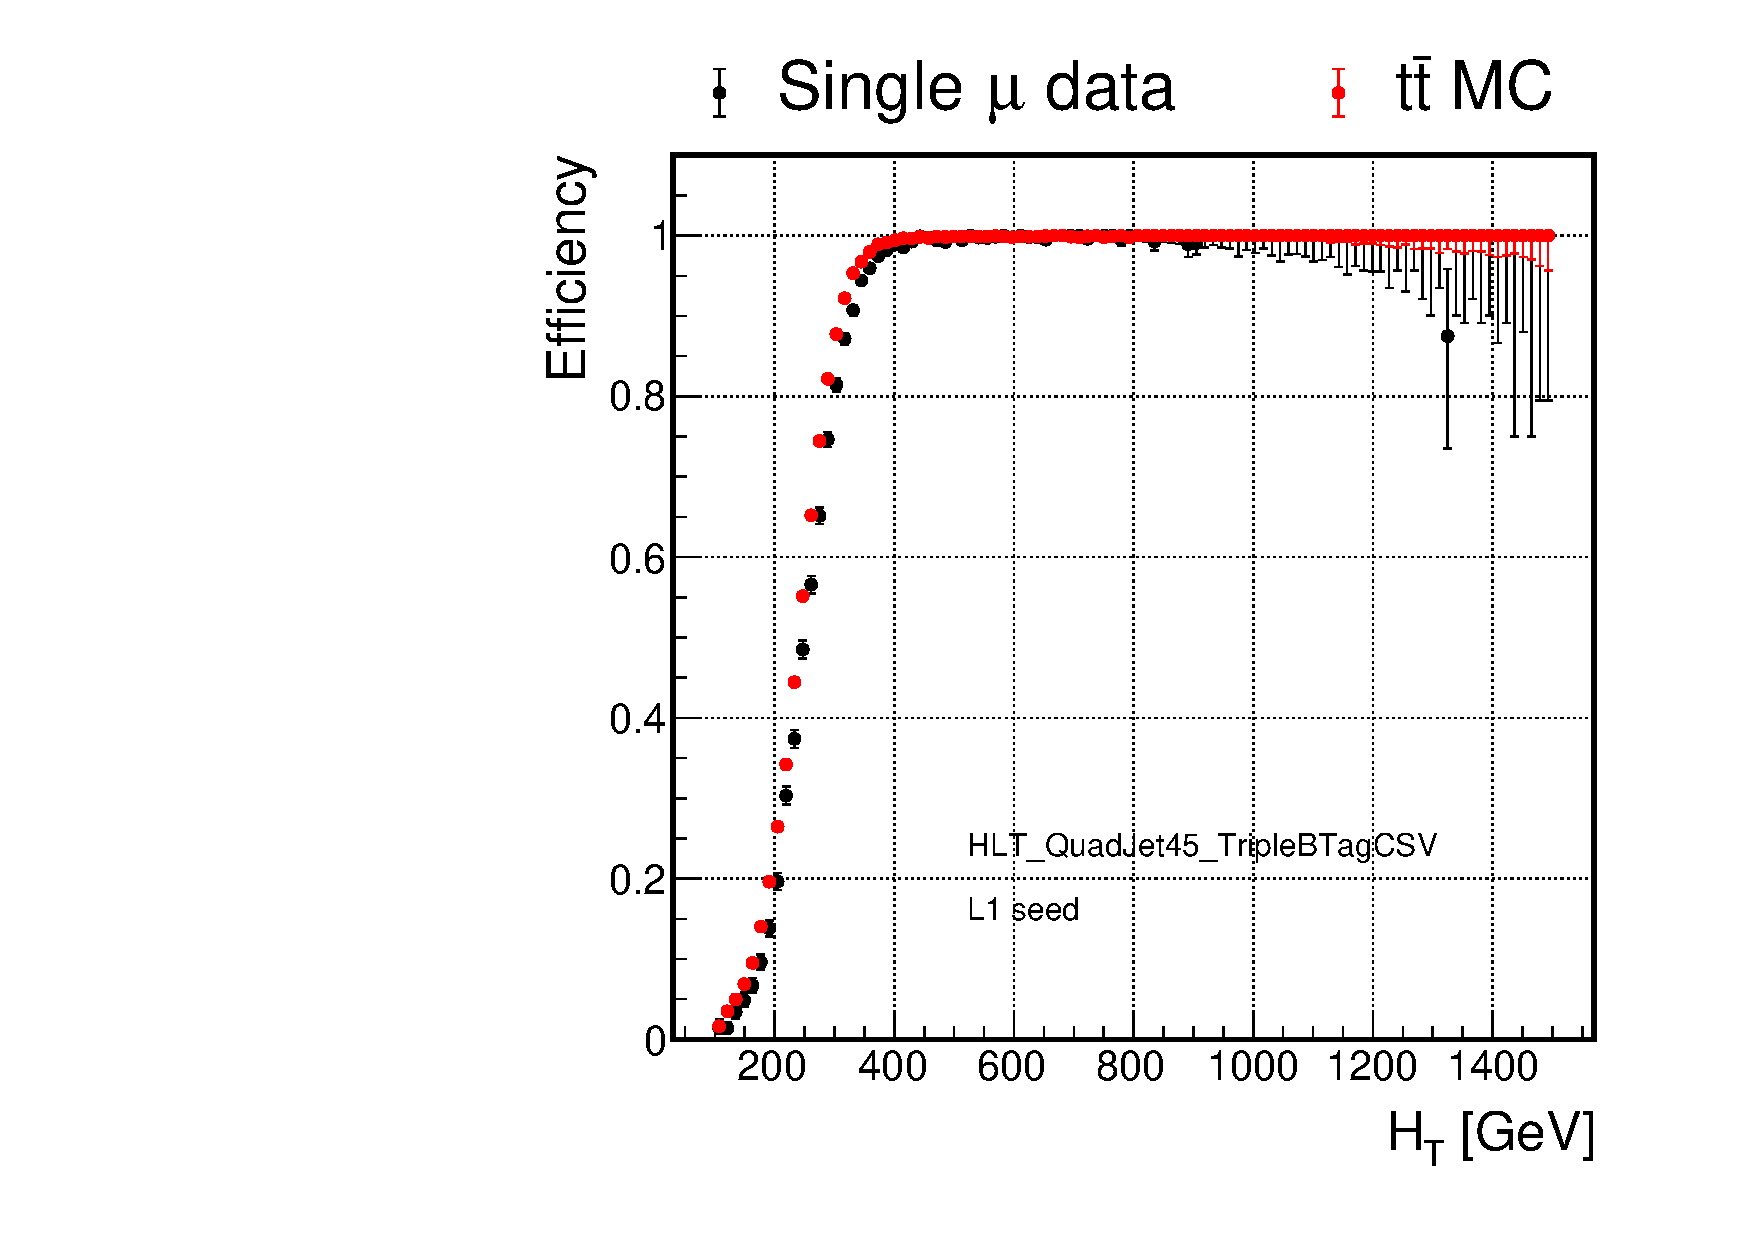
\includegraphics[width=0.3\textwidth]{Figures/AnalysisStrategy/triggereff/plots_2016/Quad45_Efficiency_L1filterHT.pdf}
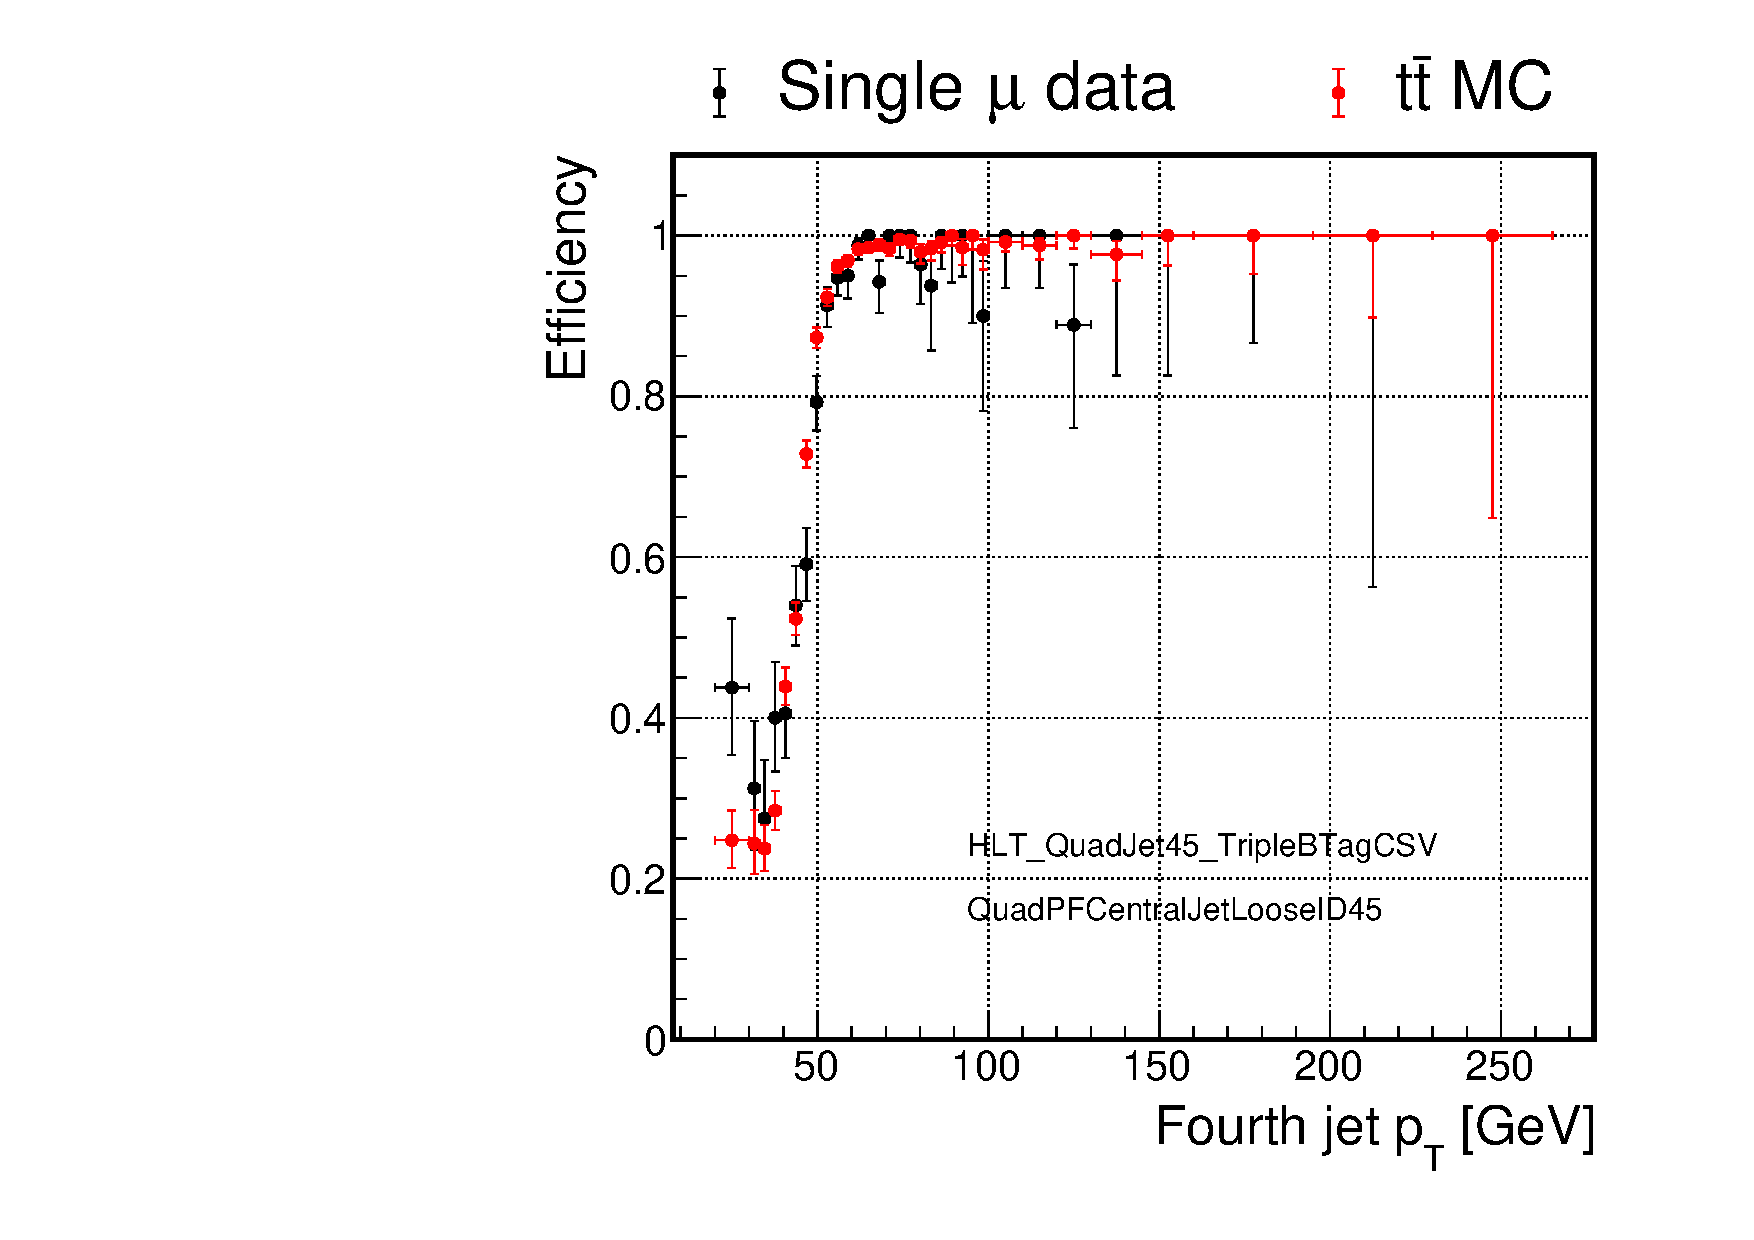
\includegraphics[width=0.3\textwidth]{Figures/AnalysisStrategy/triggereff/plots_2016/Quad45_Efficiency_QuadPFCentralJetLooseID45.pdf}
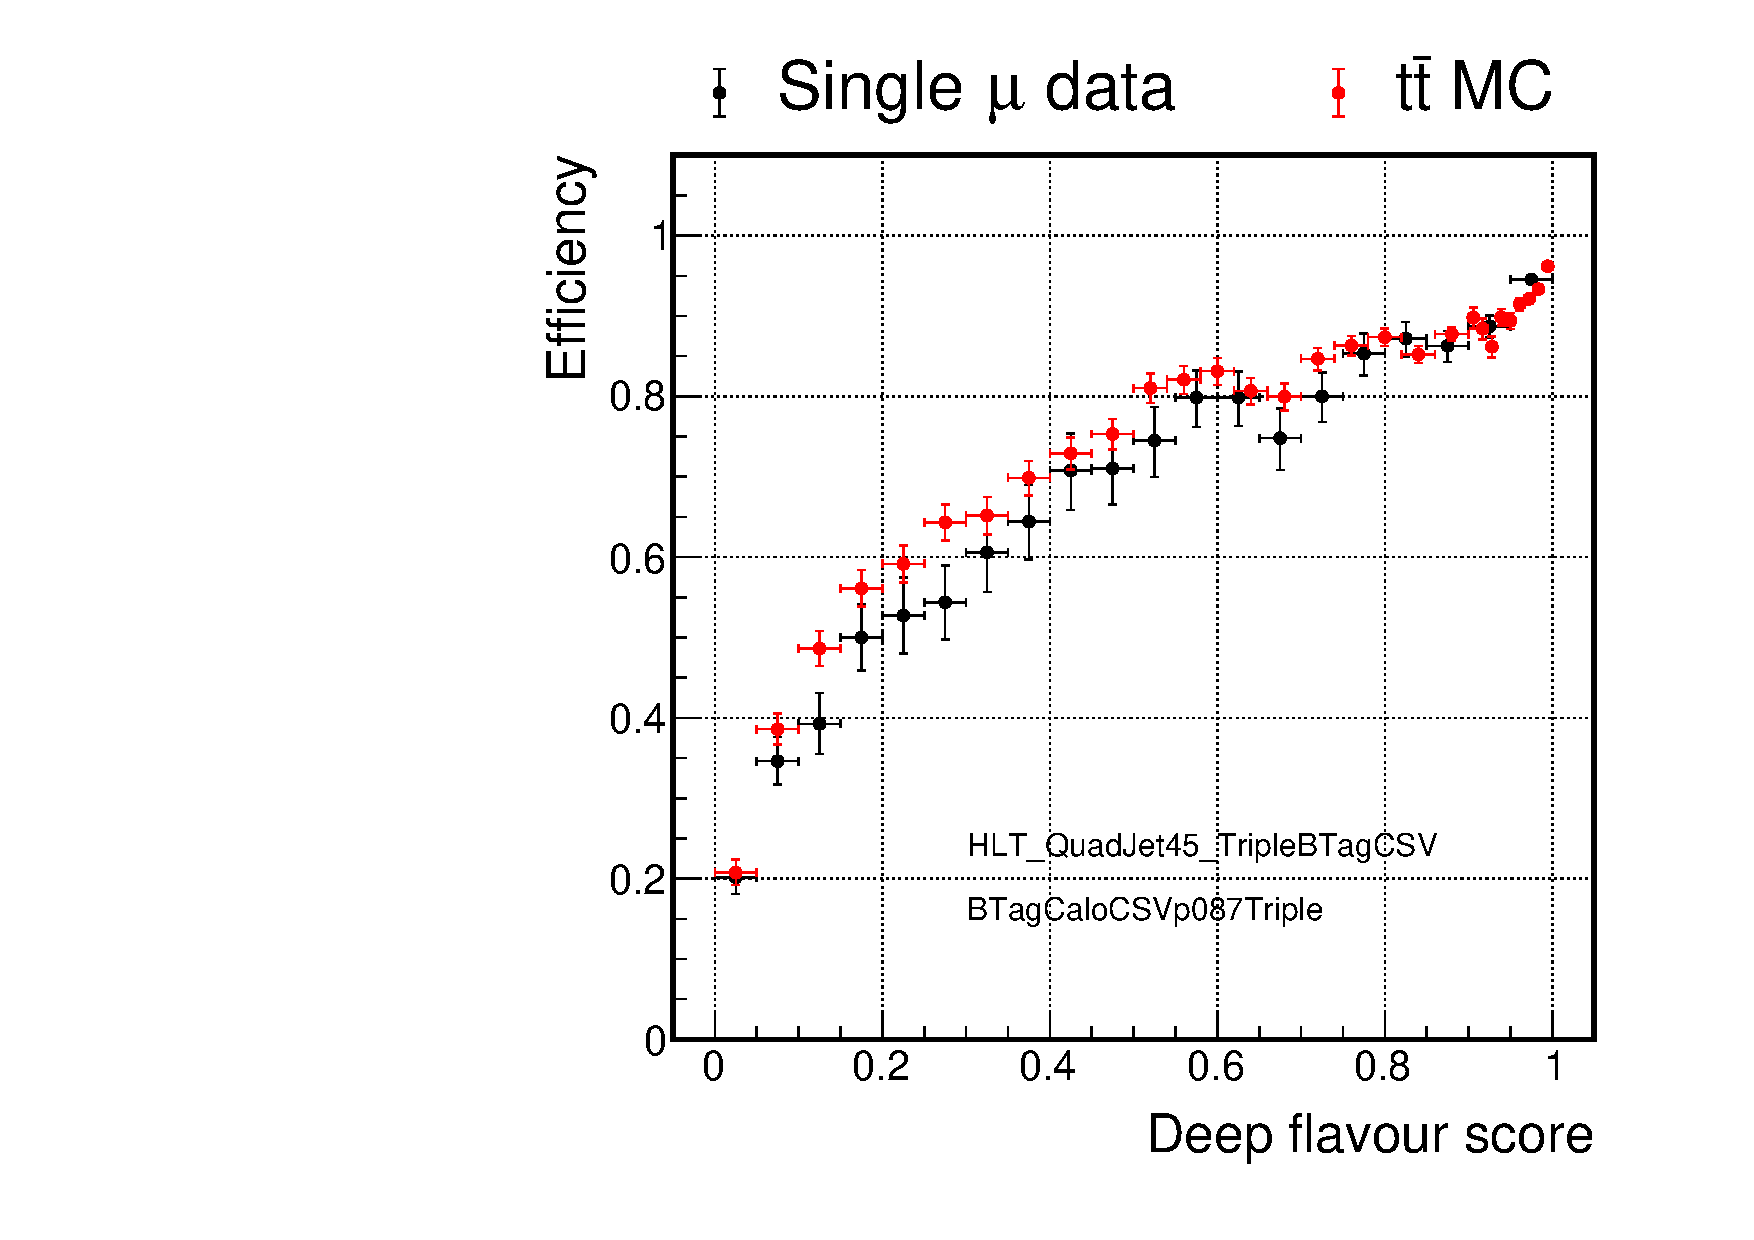
\includegraphics[width=0.3\textwidth]{Figures/AnalysisStrategy/triggereff/plots_2016/Quad45_Efficiency_BTagCaloCSVp087Triple.pdf}\\
      \end{subfigure}
      \begin{subfigure}{\textwidth}
  \centering
          \caption{}
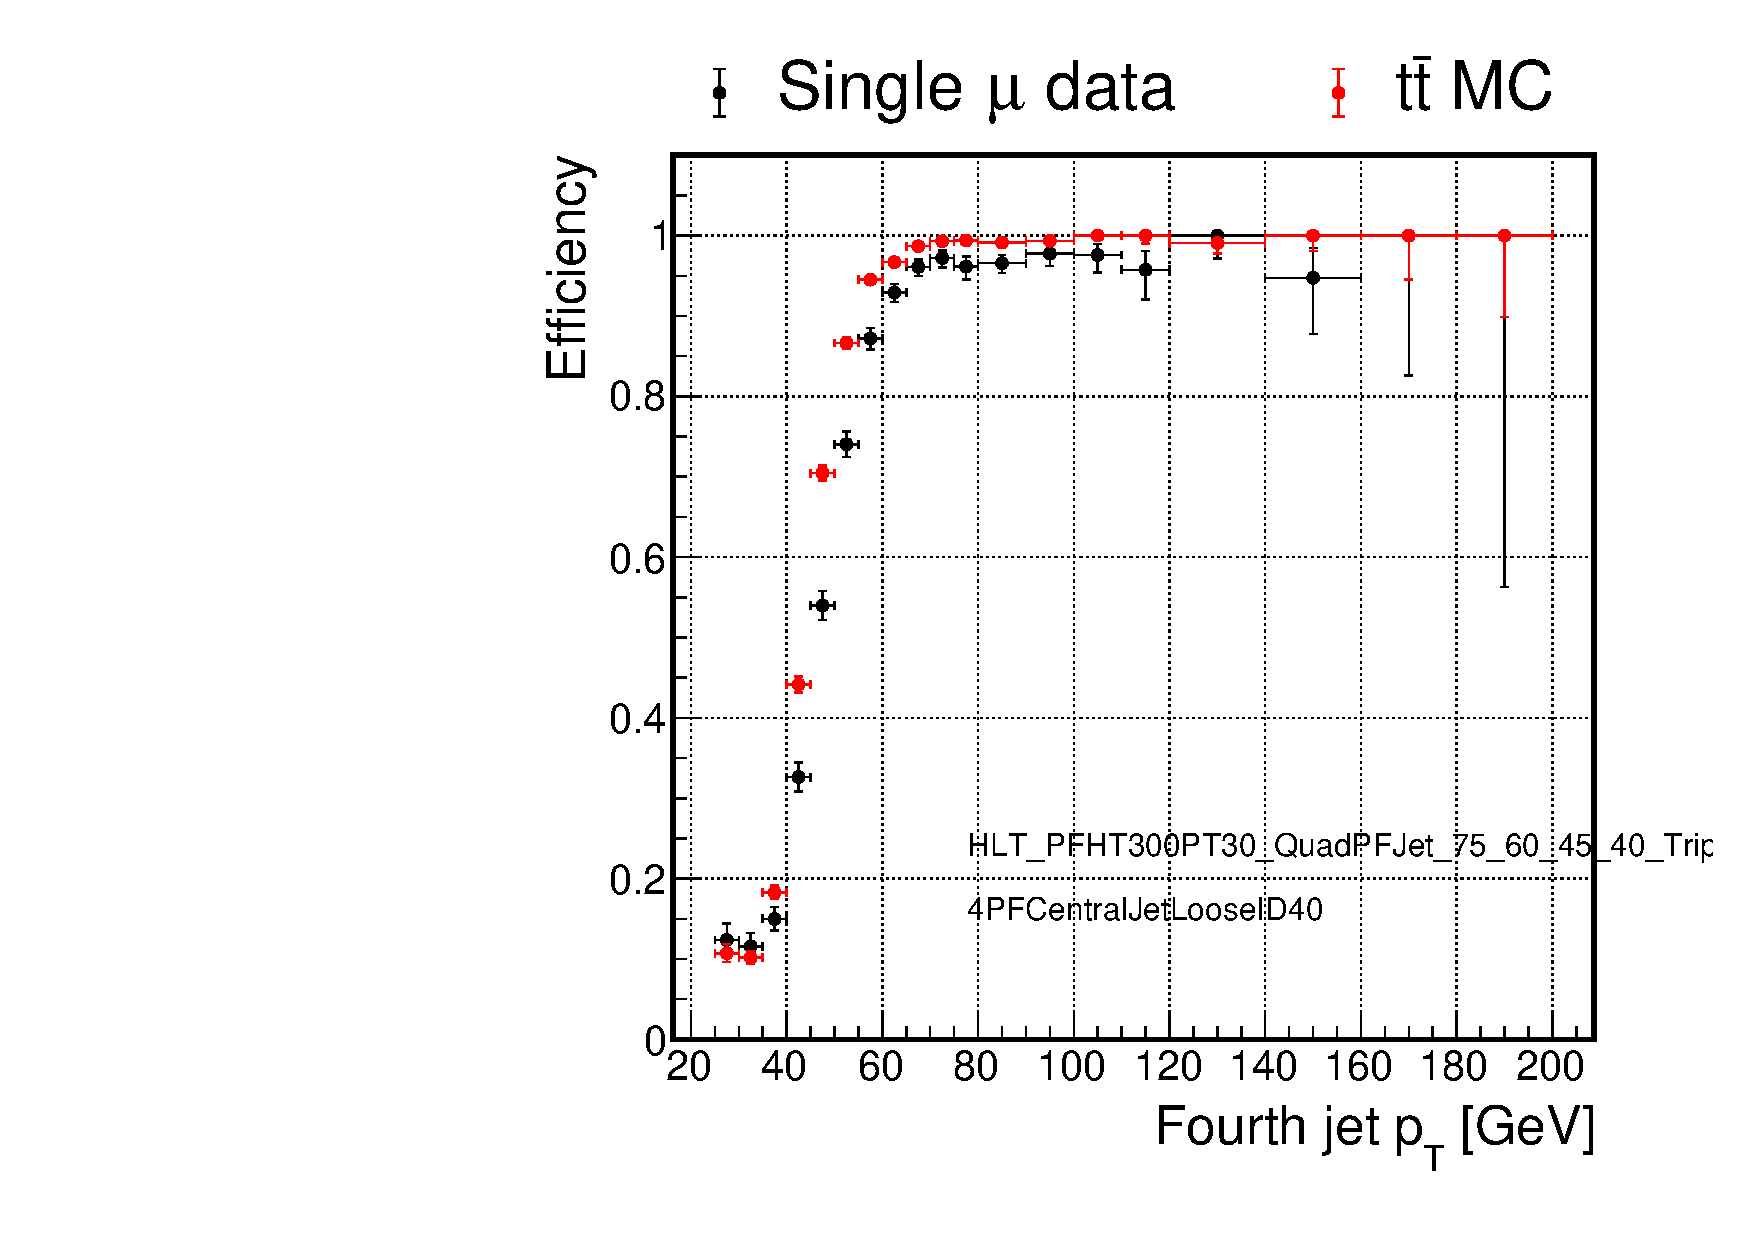
\includegraphics[width=0.3\textwidth]{Figures/AnalysisStrategy/triggereff/plots_2017/Quad_75_60_45_40_3b_Efficiency_4PFCentralJetLooseID40.pdf}
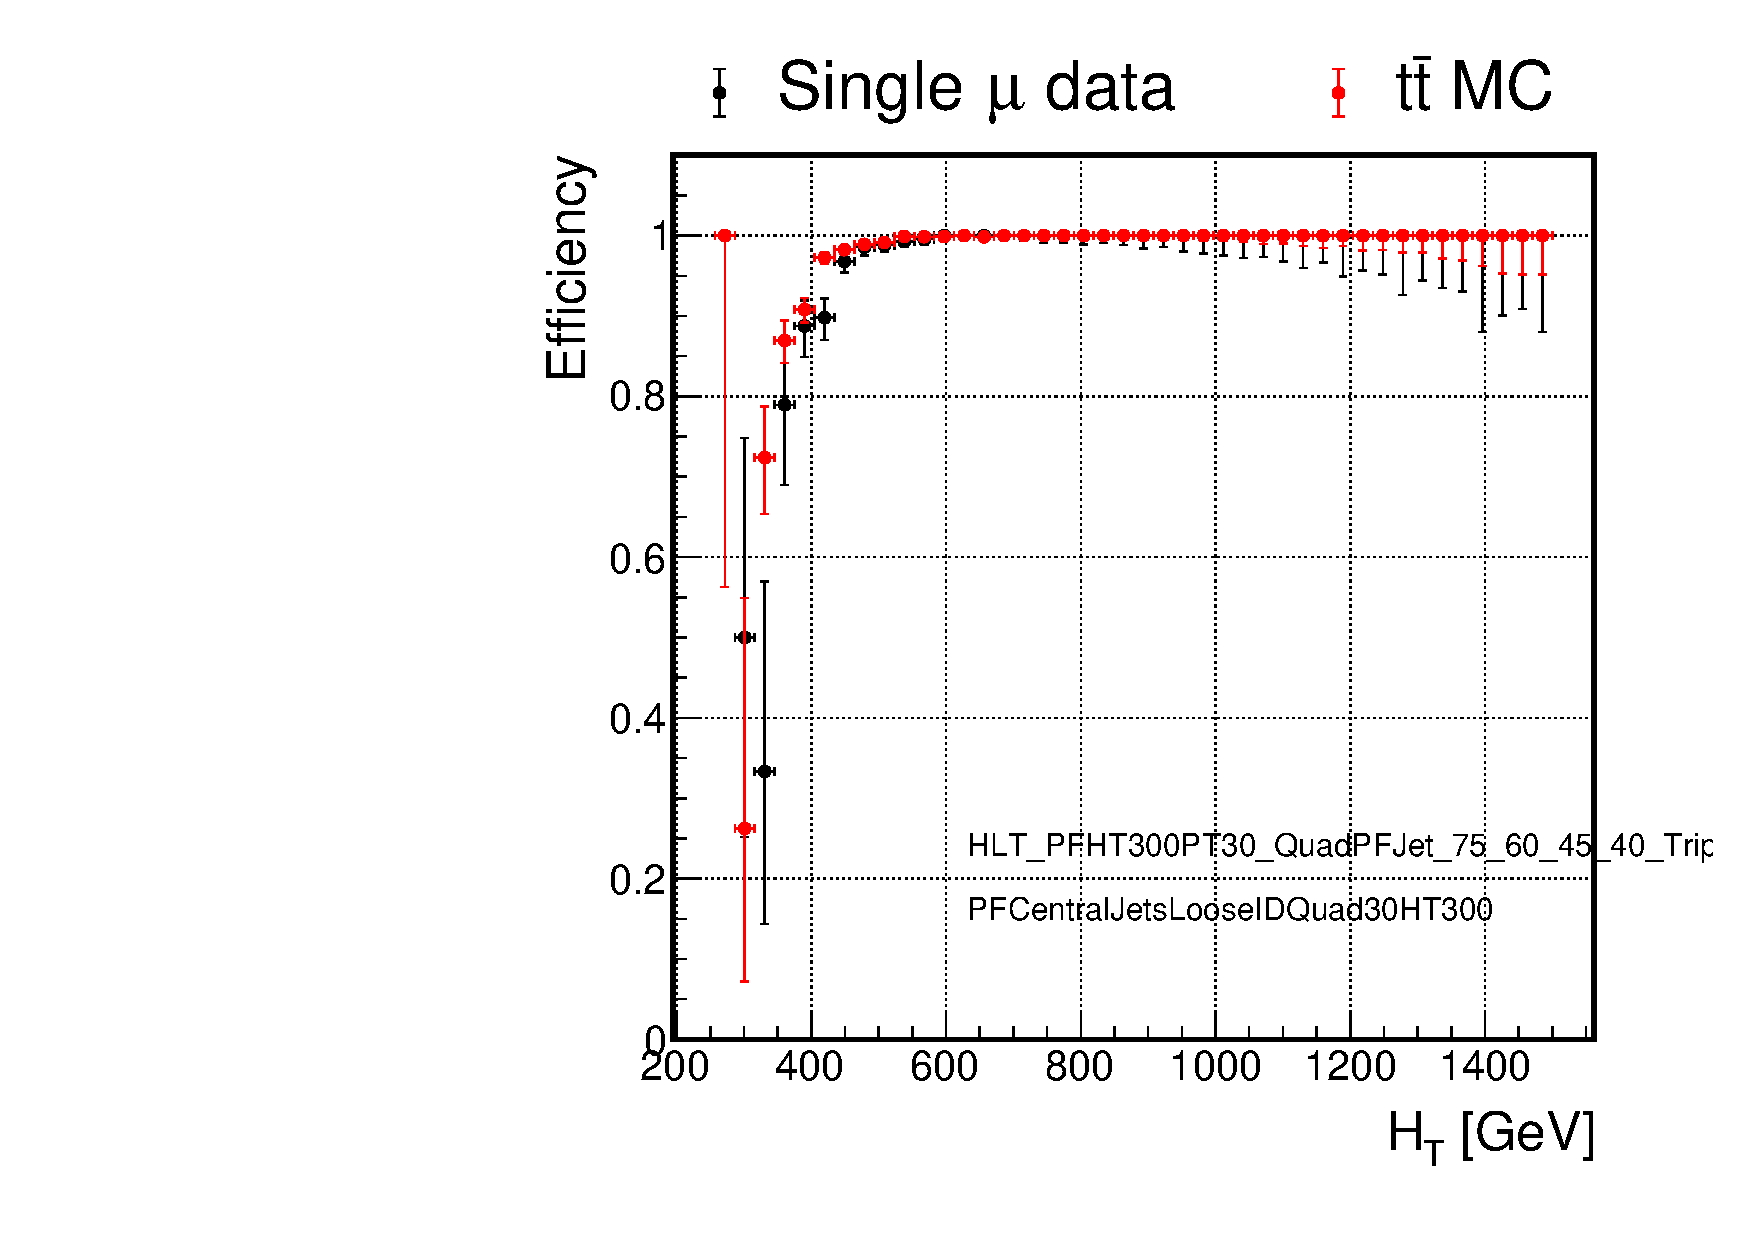
\includegraphics[width=0.3\textwidth]{Figures/AnalysisStrategy/triggereff/plots_2017/Quad_75_60_45_40_3b_Efficiency_PFCentralJetsLooseIDQuad30HT300.pdf}
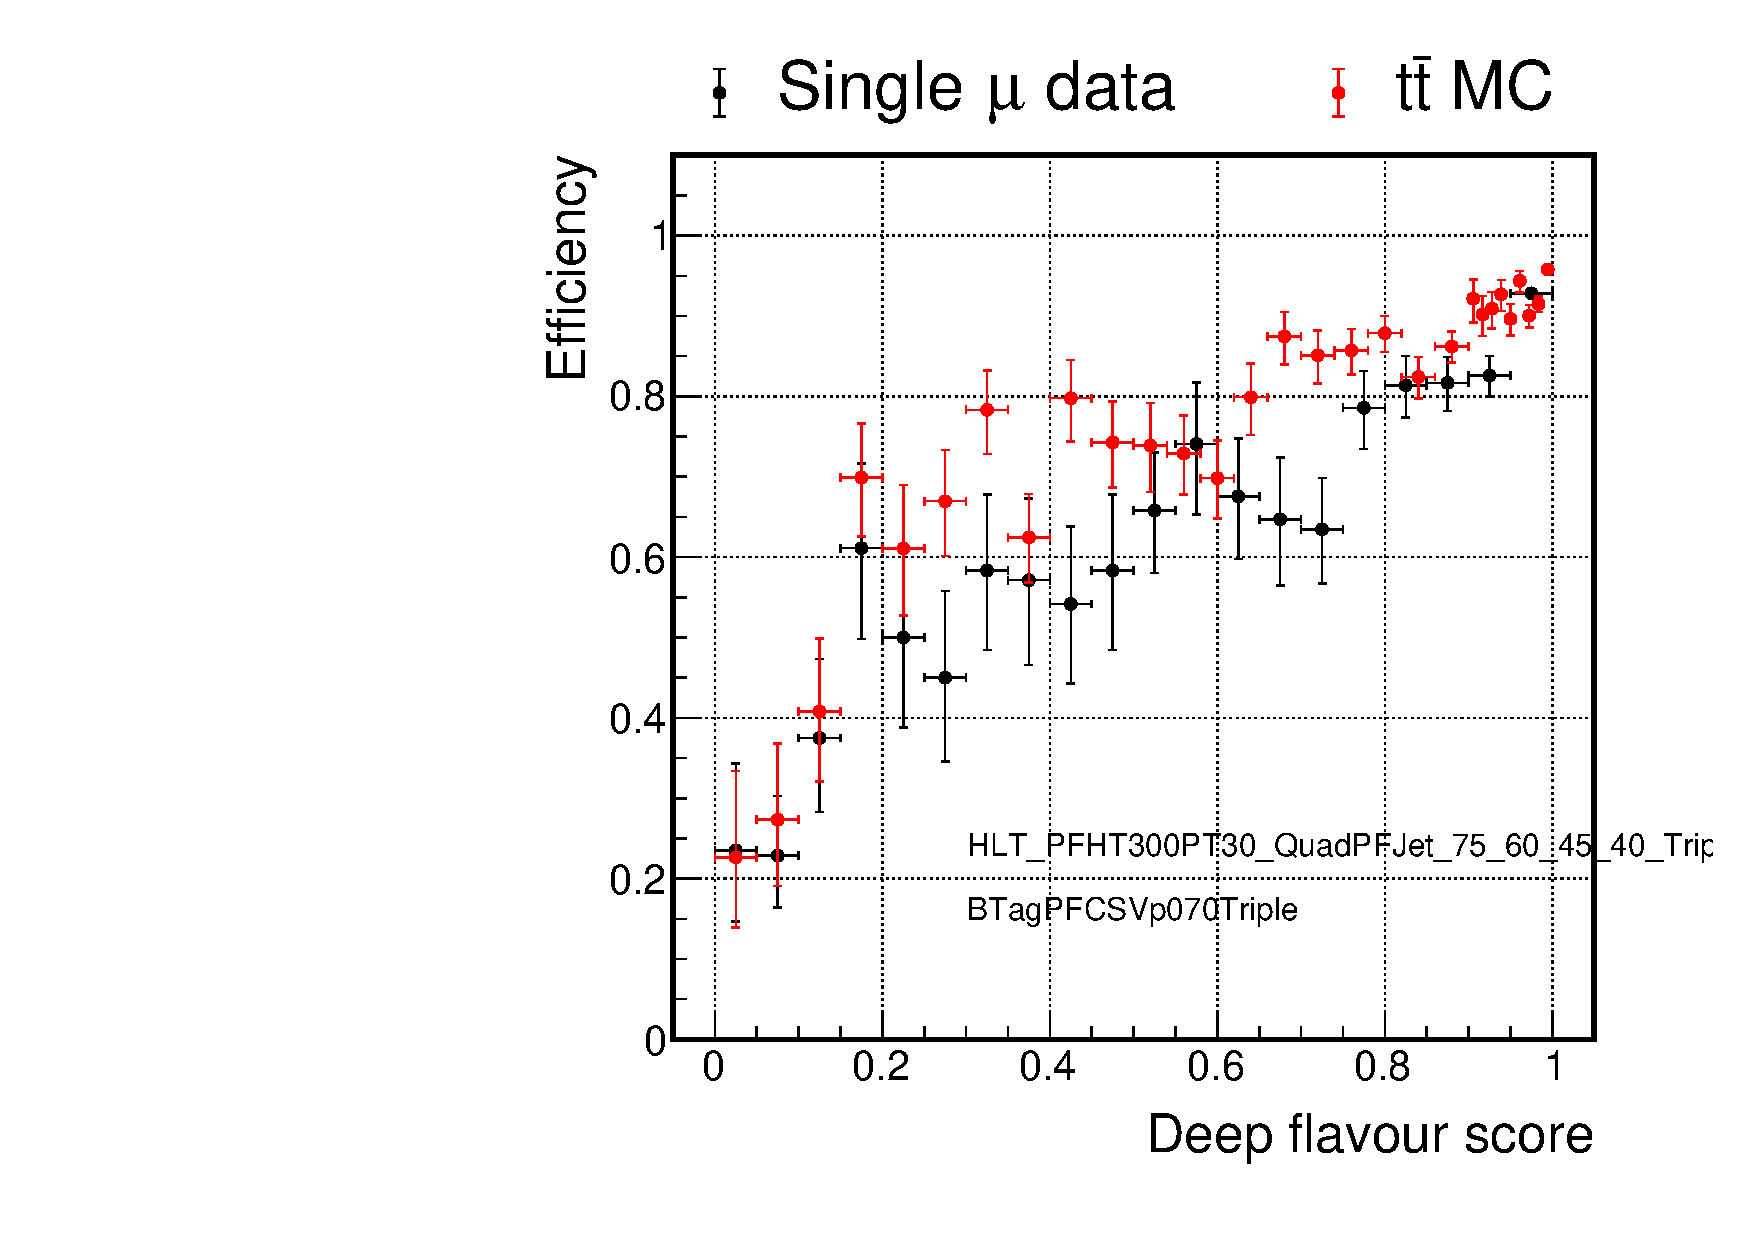
\includegraphics[width=0.3\textwidth]{Figures/AnalysisStrategy/triggereff/plots_2017/Quad_75_60_45_40_3b_Efficiency_BTagPFCSVp070Triple.pdf}\\
      \end{subfigure}
      \begin{subfigure}{\textwidth}
  \centering
            \caption{}
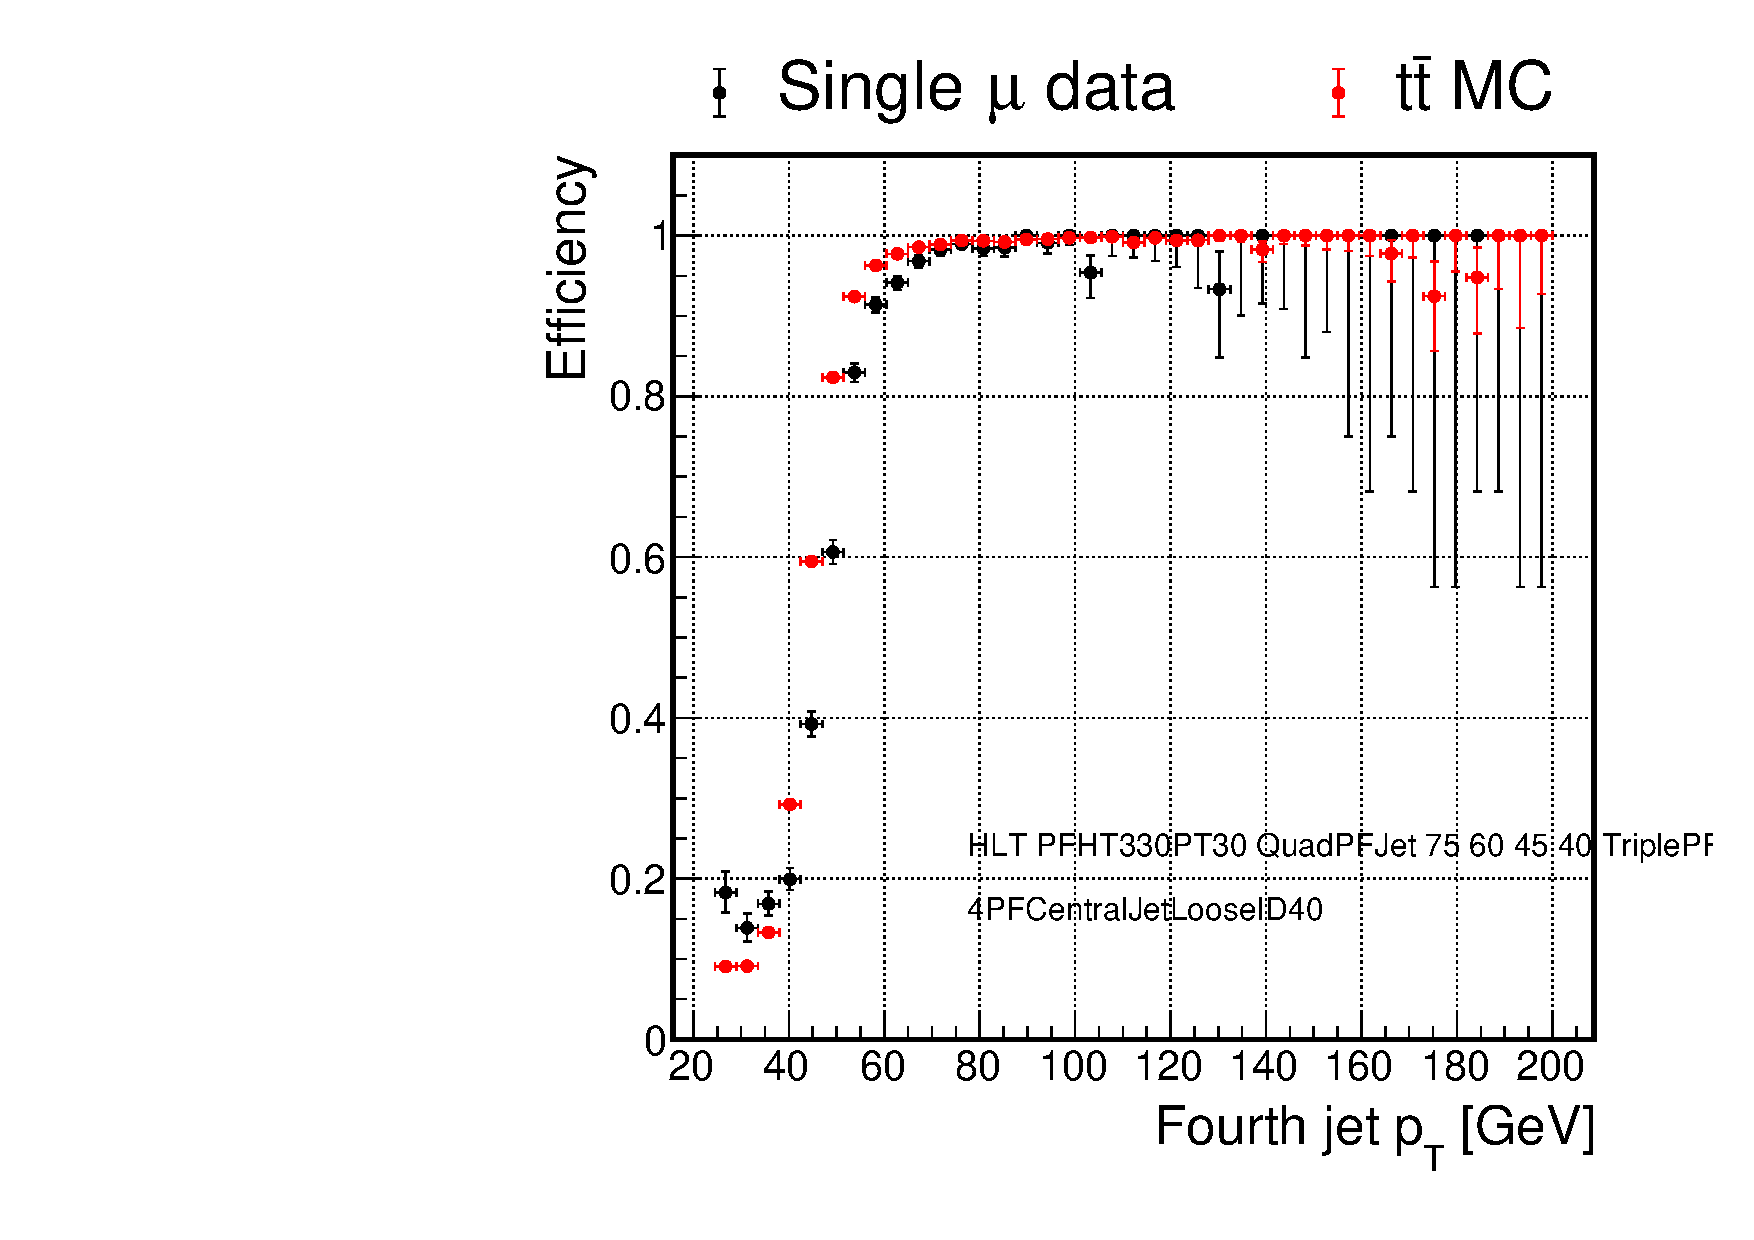
\includegraphics[width=0.3\textwidth]{Figures/AnalysisStrategy/triggereff/plots_2018/Quad_75_60_45_40_3b_Efficiency_4PFCentralJetLooseID40.pdf}
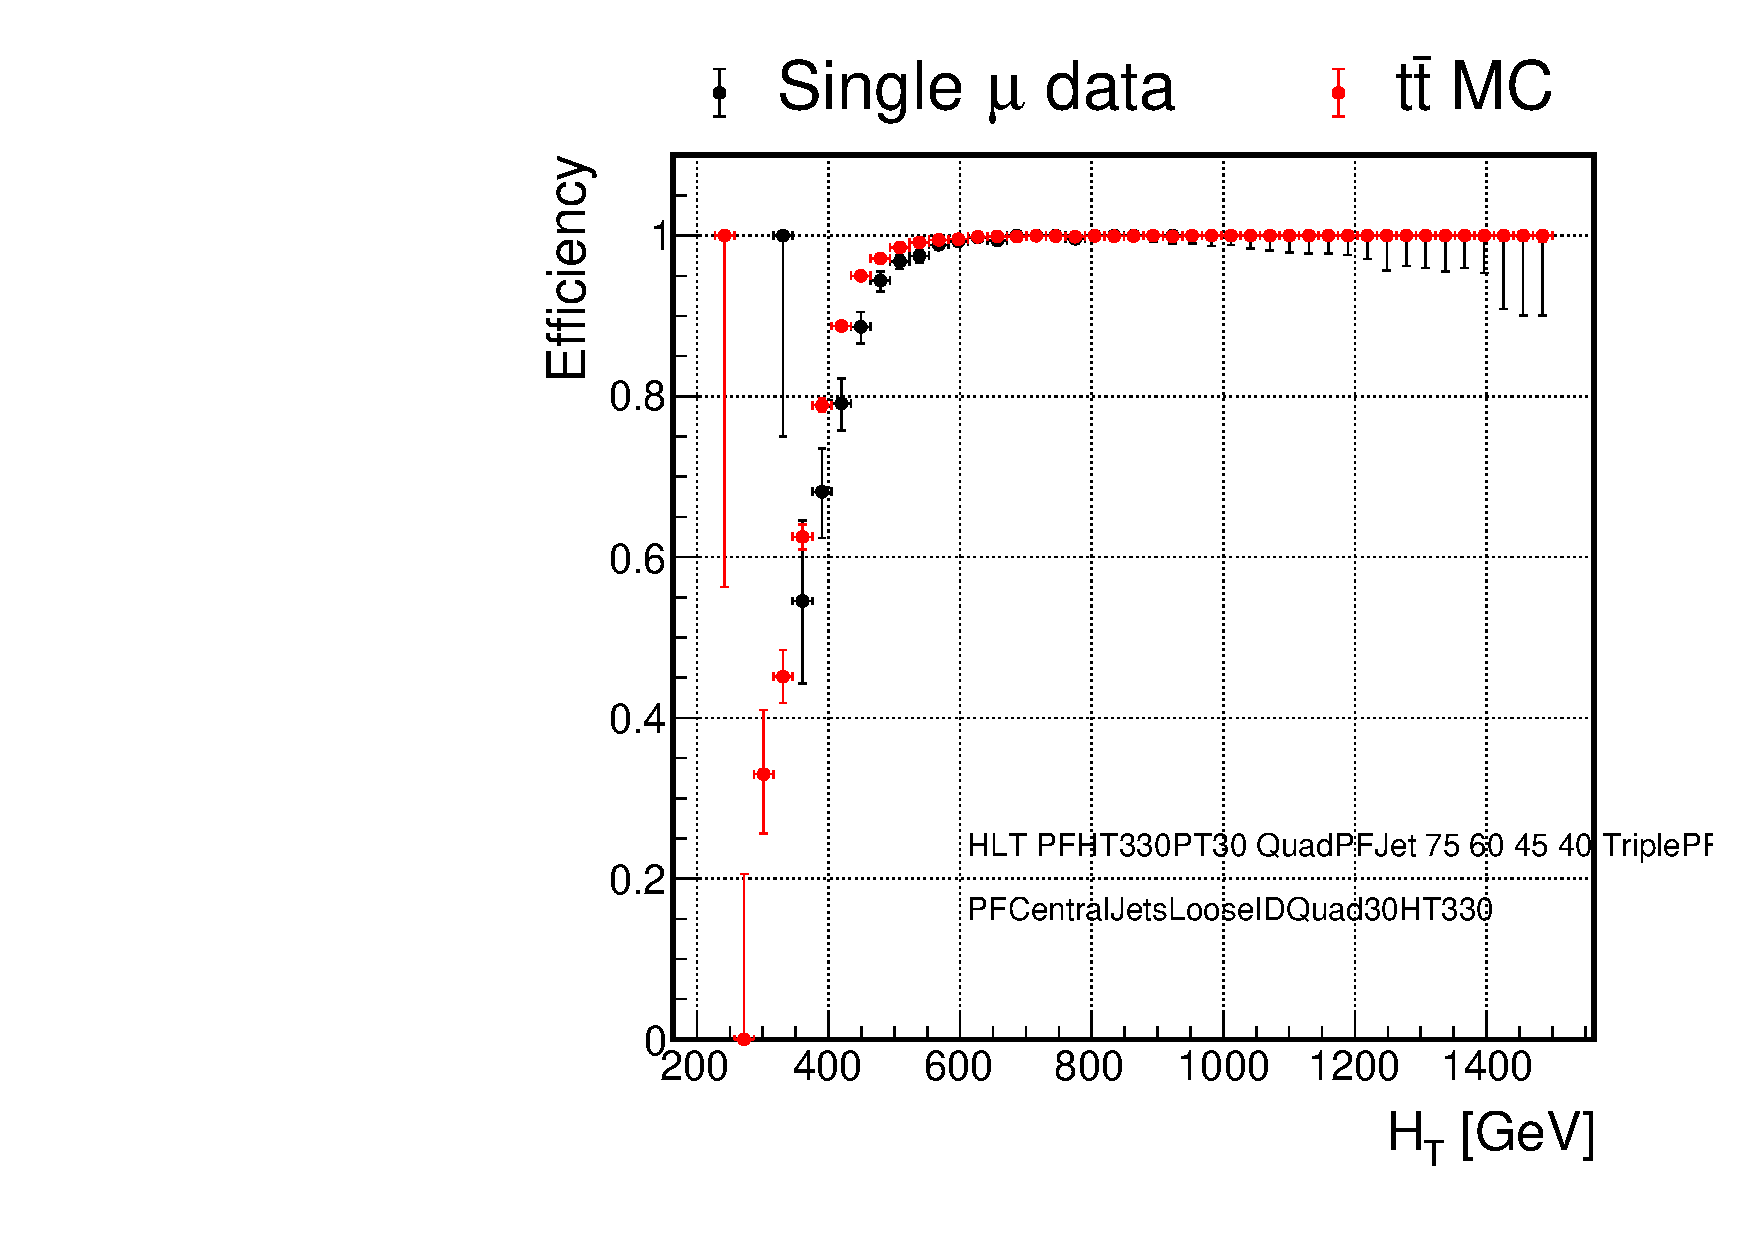
\includegraphics[width=0.3\textwidth]{Figures/AnalysisStrategy/triggereff/plots_2018/Quad_75_60_45_40_3b_Efficiency_PFCentralJetsLooseIDQuad30HT330.pdf}
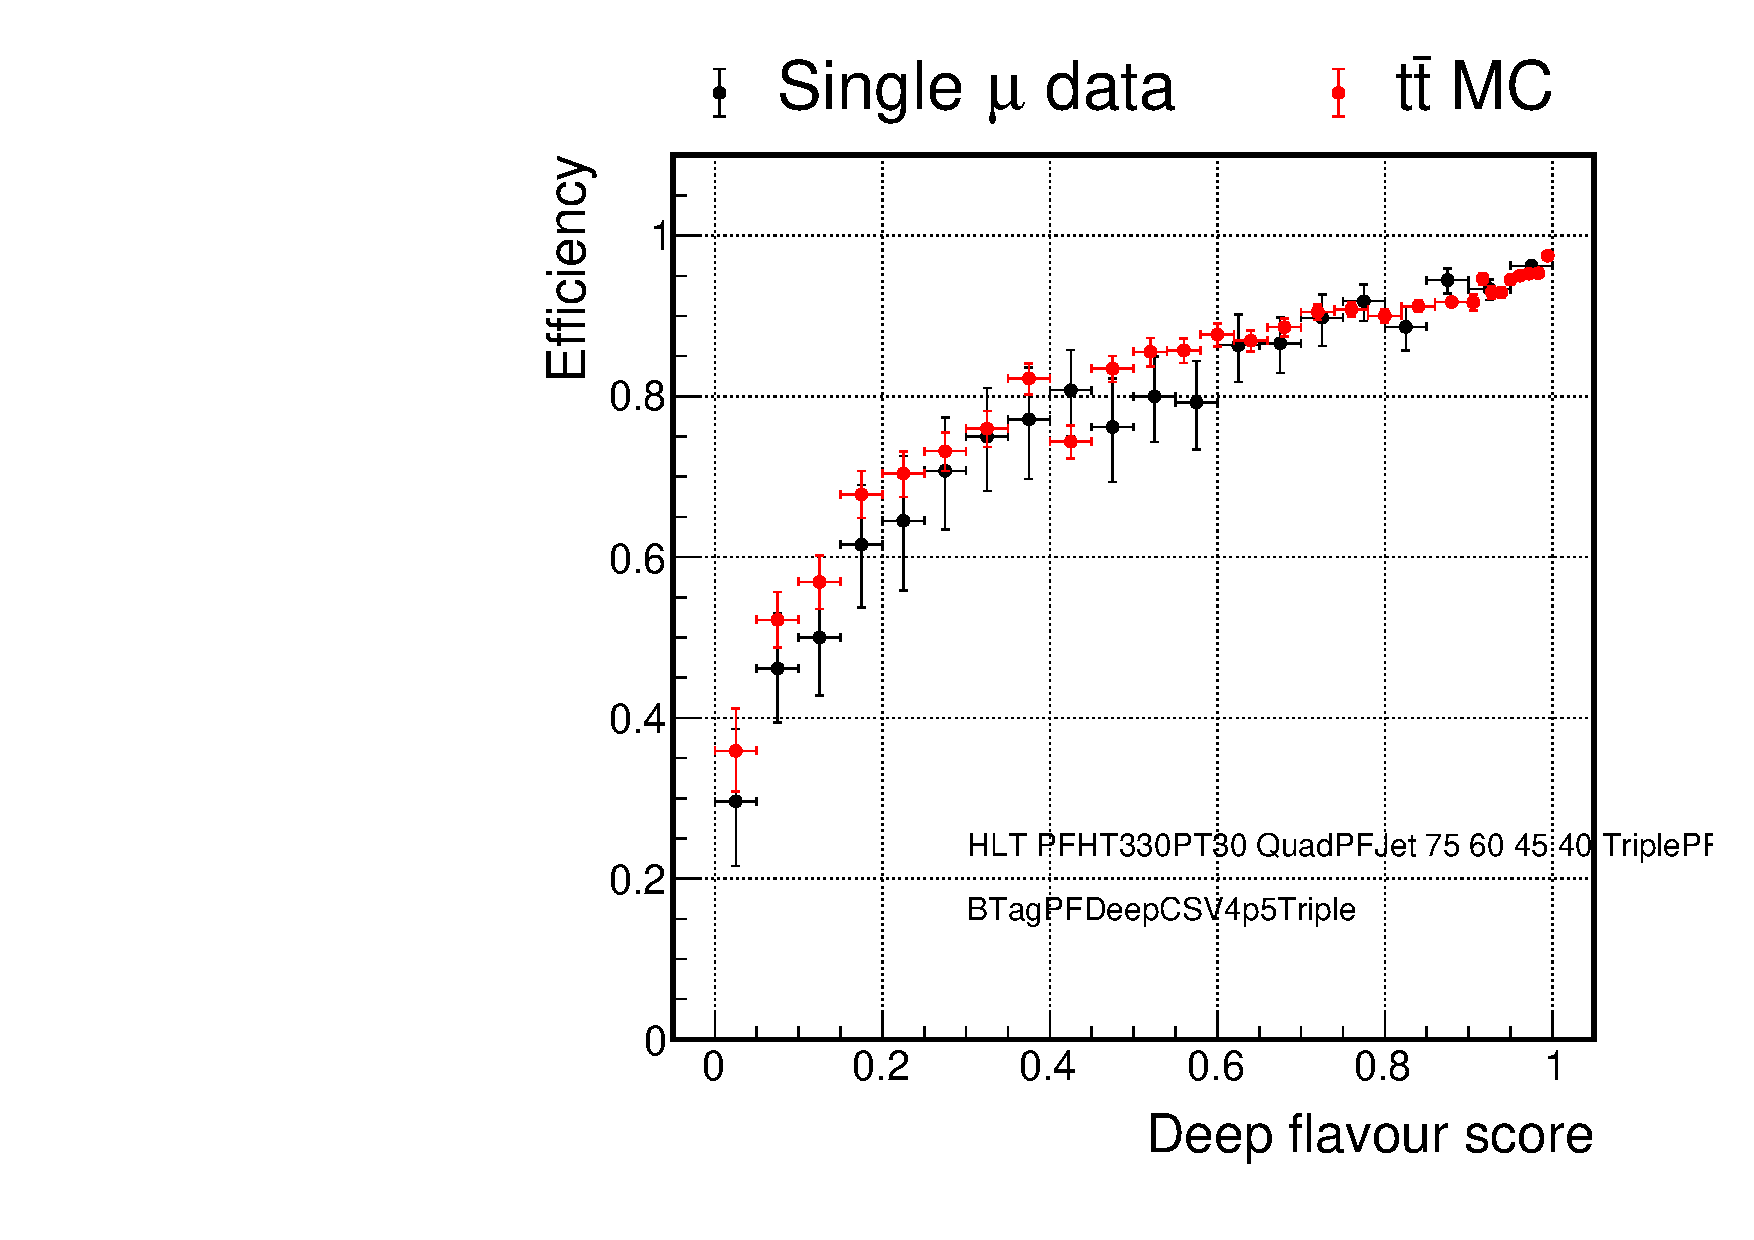
\includegraphics[width=0.3\textwidth]{Figures/AnalysisStrategy/triggereff/plots_2018/Quad_75_60_45_40_3b_Efficiency_BTagPFDeepCSV4p5Triple.pdf}
      \end{subfigure}
\caption[Examples of the measured trigger filter efficiency in single muon ($\mu$) data and top-quark pair ($\ttbar$) MC simulation events]{\label{fig:run2triggerefficiency}Examples of the measured trigger filter efficiency in single muon ($\mu$) data (black) and top-quark pair ($\ttbar$) MC simulation (red) events. A) HLT\_QuadJet45\_TripleBTagCSV filters used in 2016, B) HLT\_PFHT300PT30\_QuadPFJet\_75\_60\_45\_40\_TriplePFBTagCSV filters used in 2017, C) HLT\_PFHT330PT30\_QuadPFJet\_75\_60\_45\_40\_TriplePFBTagDeepCSV filters used in 2018.}
\end{figure}


\clearpage

\begin{figure}[htp!]%toupdate
\centering
\captionsetup[subfigure]{justification=centering}
\subfloat[]{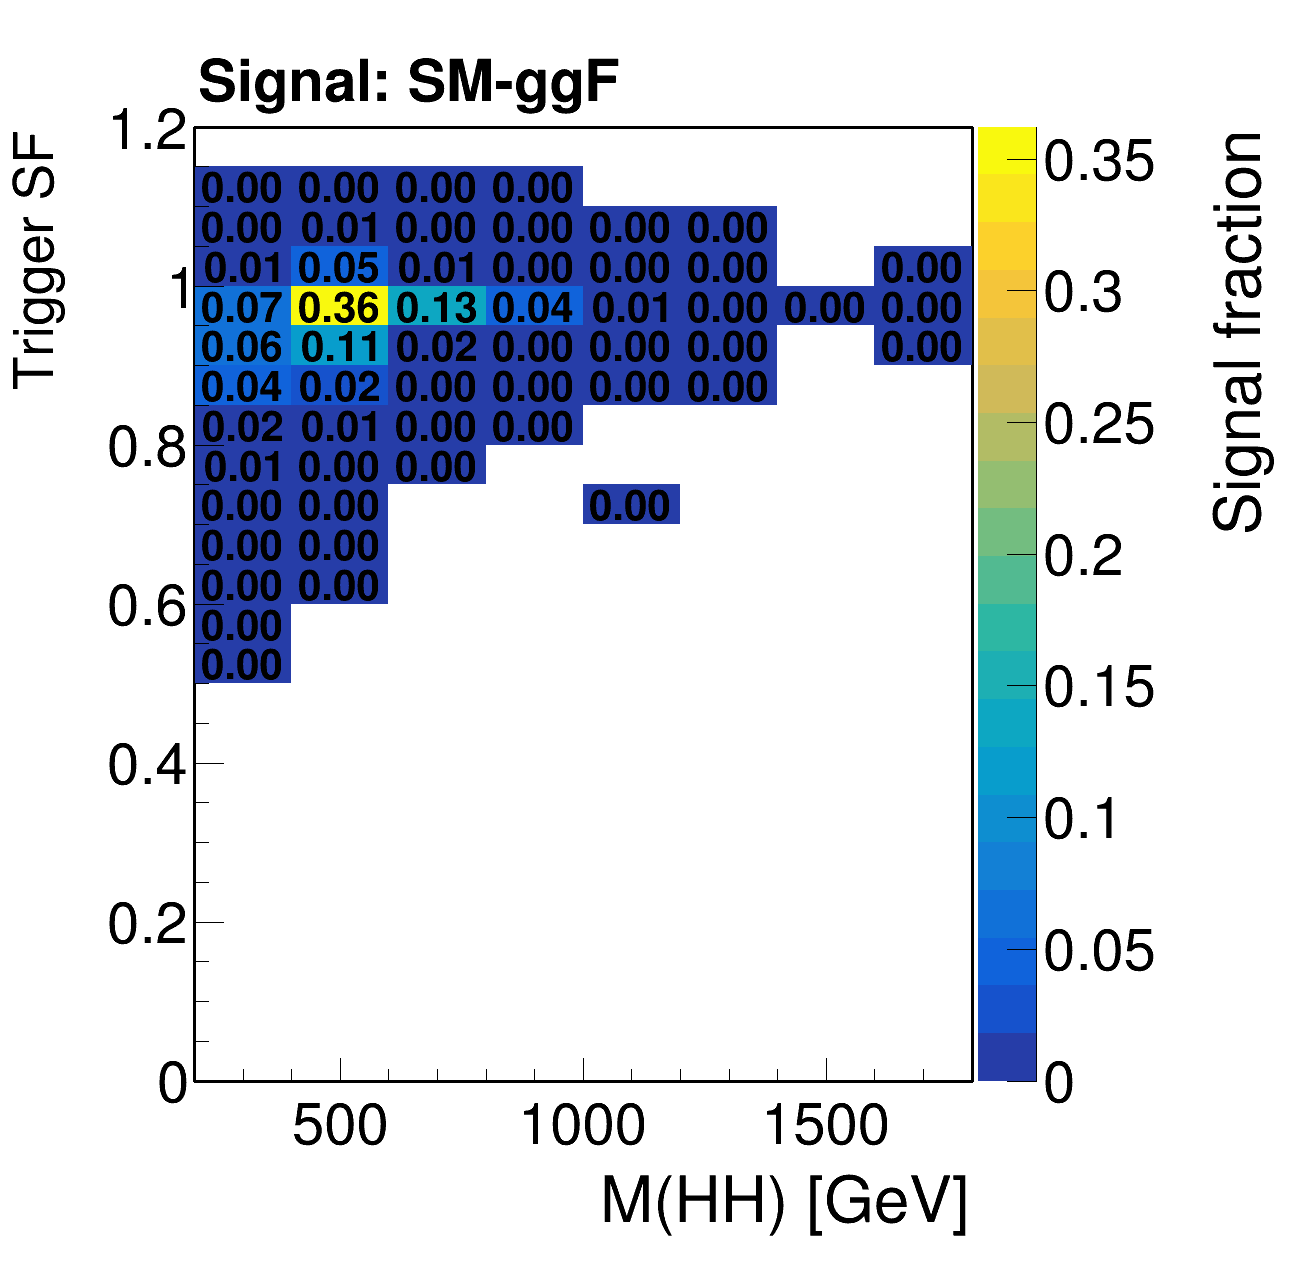
\includegraphics[width=0.32\textwidth]{Figures/AnalysisStrategy/triggersfclosure/plot_2016_SFvsmHH.png}}
\subfloat[]{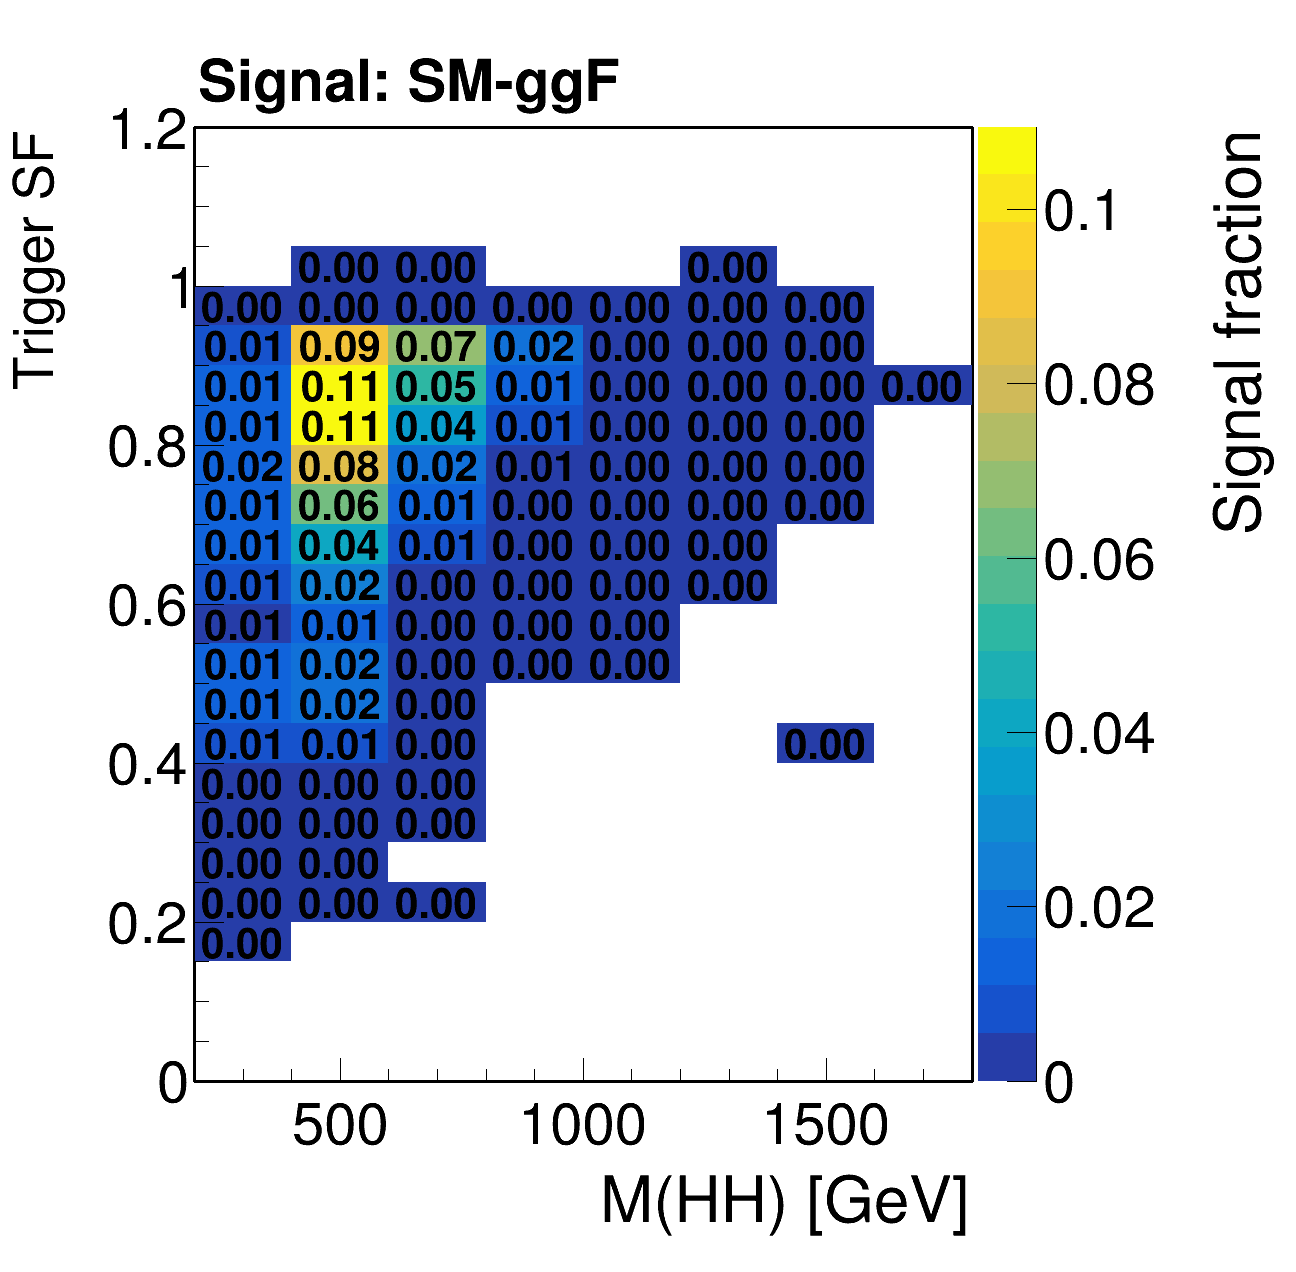
\includegraphics[width=0.32\textwidth]{Figures/AnalysisStrategy/triggersfclosure/plot_2017_SFvsmHH.png}}
\subfloat[]{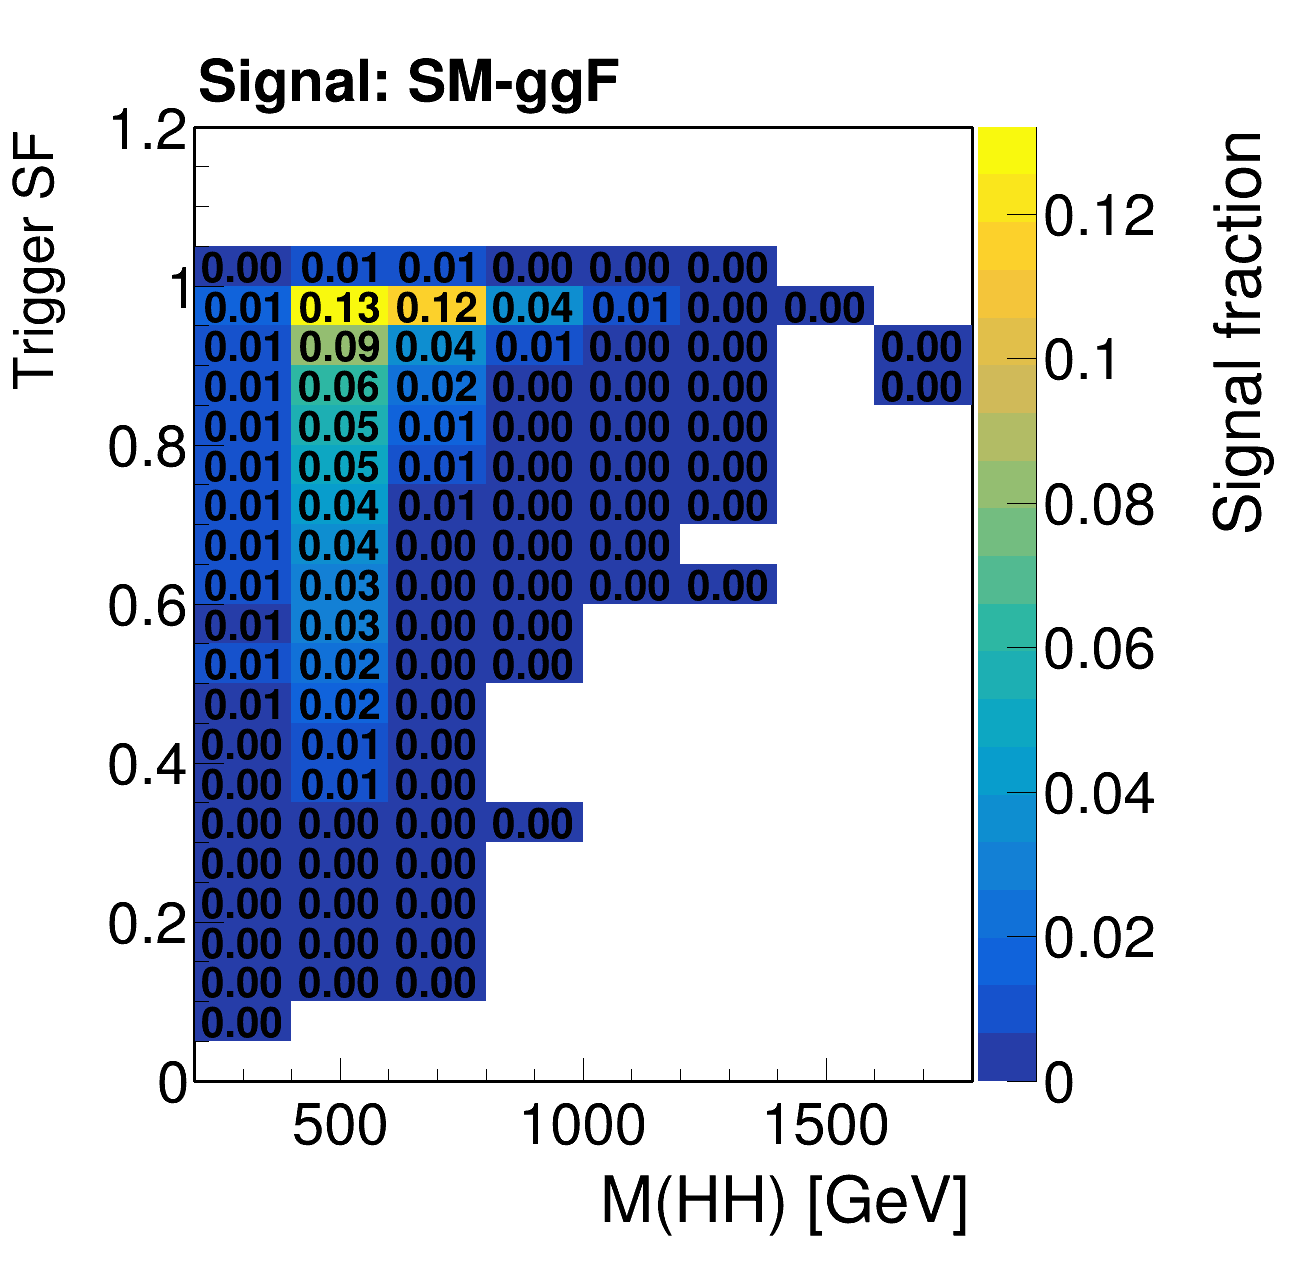
\includegraphics[width=0.32\textwidth]{Figures/AnalysisStrategy/triggersfclosure/plot_2018_SFvsmHH.png}}
\caption[Fraction of SM ggF signal events that are attribute a specific value of the trigger scale factor as function of the Higgs boson pair mass.]{Fraction of SM ggF signal events (z-axis) that are attributed a specific value of the trigger scale factor (y-axis) as a function of Higgs boson pair mass (x-axis). A) 2016 trigger, B) 2017 trigger and C) 2018 trigger.}
\label{fig:triggersfs}
\end{figure}

The validation of the trigger MC efficiency measurement is carried out by a closure test performed in $\ttbar$ and signal simulated events passing the event preselection requirements presented in Section~\ref{sec:preselection}. The test consists of comparing the total MC efficiency obtained from the MC fits, and the one obtained from the simulated trigger bits. A very good agreement was found between the two estimations within the uncertainties in $\ttbar$ and signal closure tests. This validates the trigger MC measurement and also by proxy the usage of the trigger SFs. The closure test  for SM ggF signal events is illustrated in Figure~\ref{fig:triggermcclosure}.


\begin{figure}[htp!]%toupdate
\centering
\captionsetup[subfigure]{justification=centering}
\subfloat[]{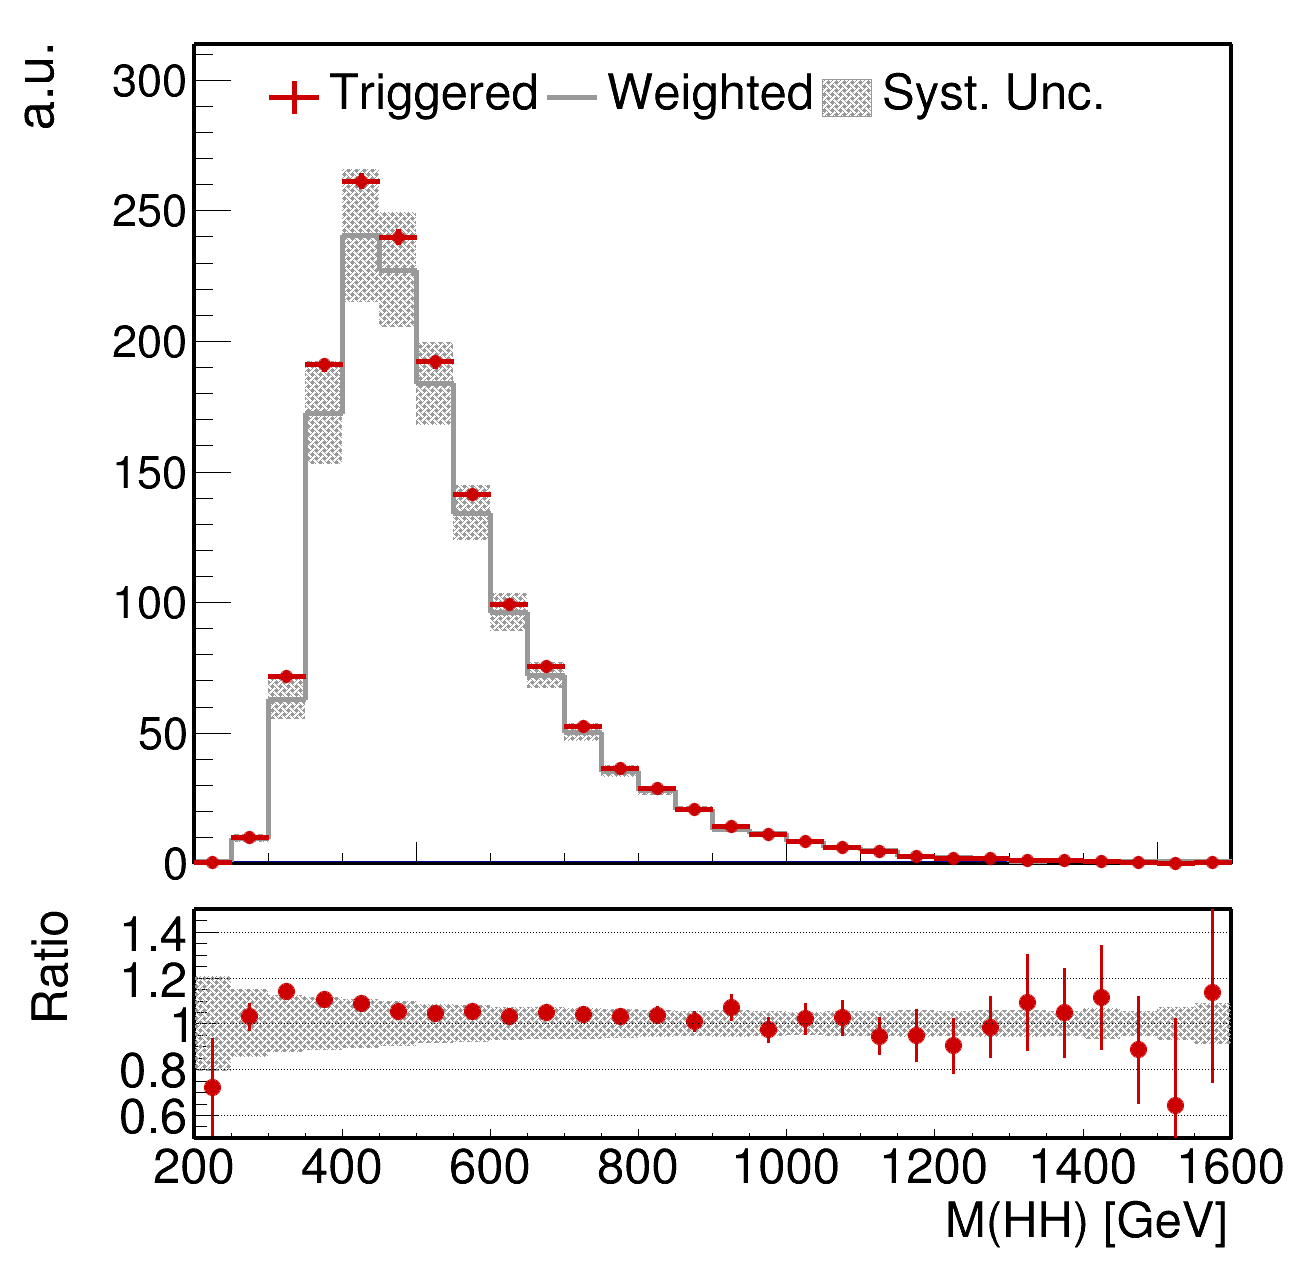
\includegraphics[width=0.33\textwidth]{Figures/AnalysisStrategy/triggersfclosure/plot_2016_mcclosure_mhh_SM-ggF.png}}
\subfloat[]{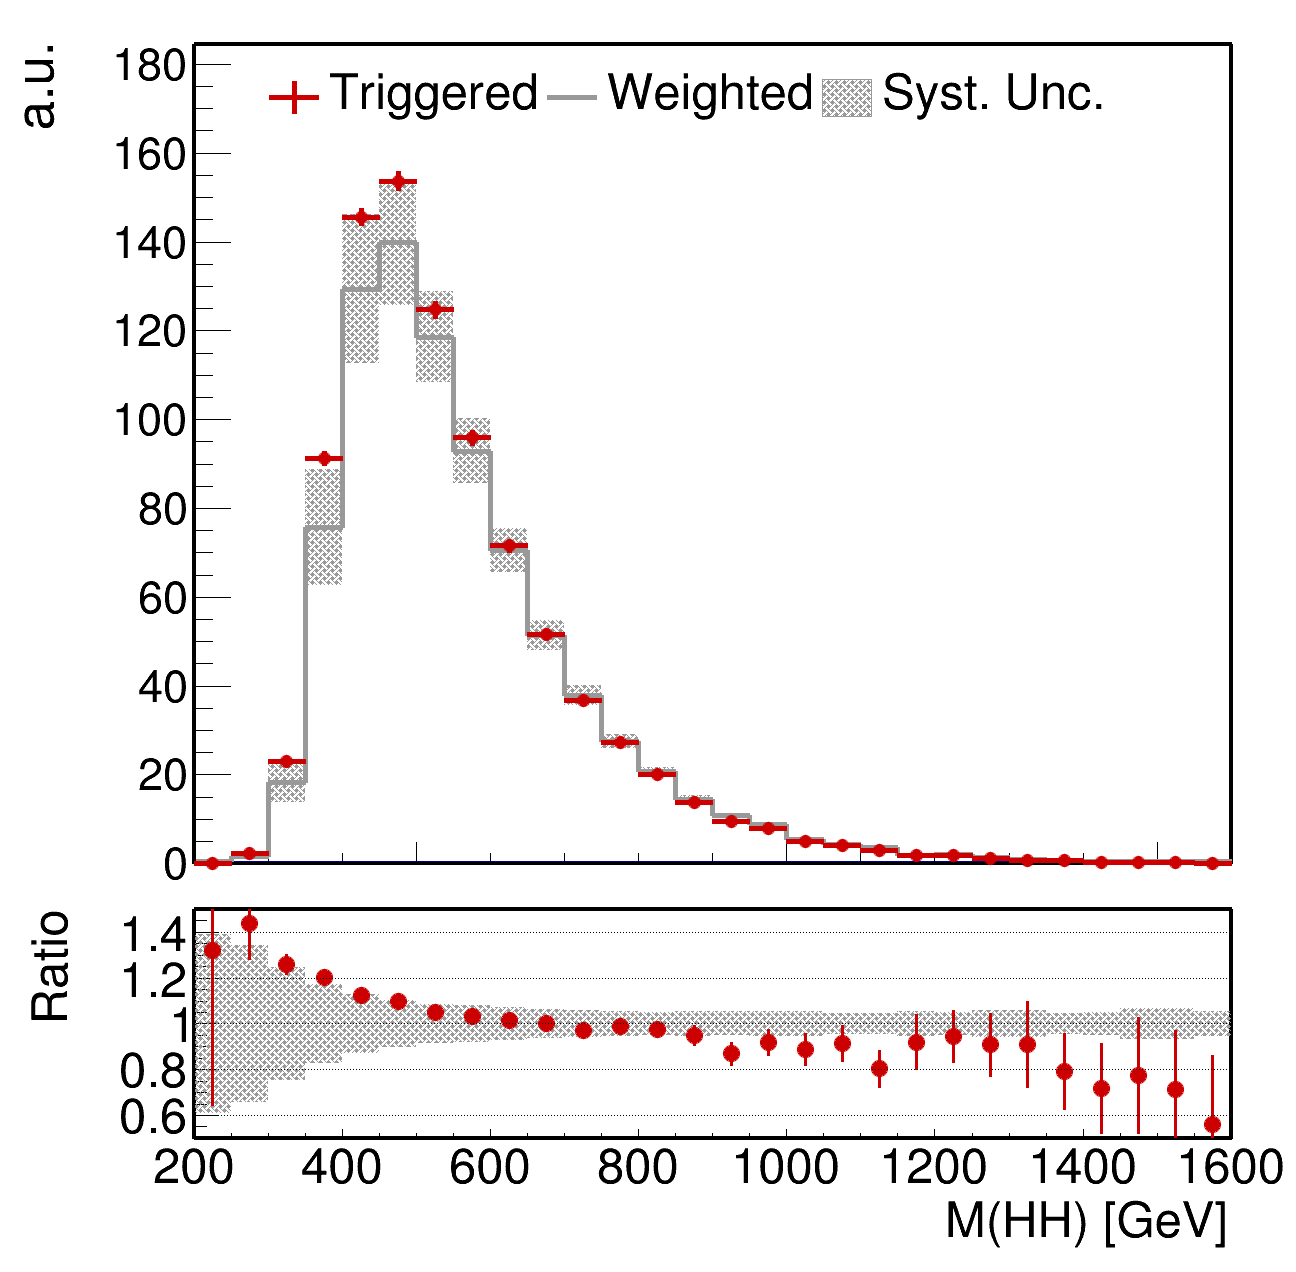
\includegraphics[width=0.33\textwidth]{Figures/AnalysisStrategy/triggersfclosure/plot_2017_mcclosure_mhh_SM-ggF.png}}
\subfloat[]{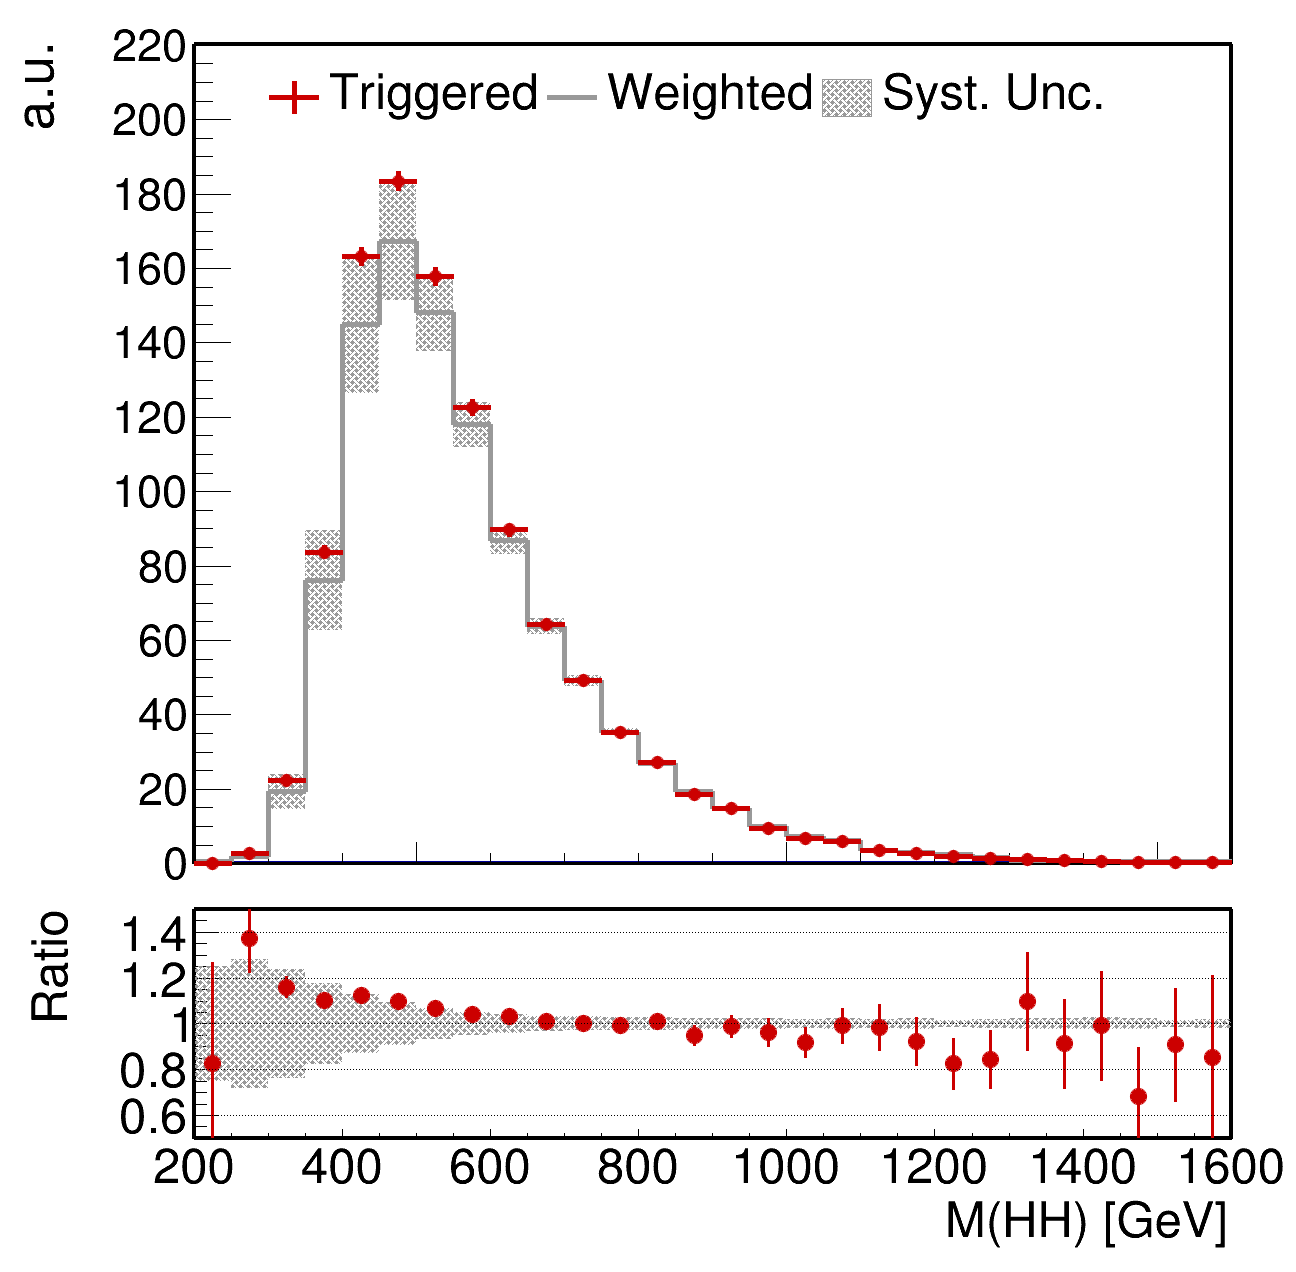
\includegraphics[width=0.33\textwidth]{Figures/AnalysisStrategy/triggersfclosure/plot_2018_mcclosure_mhh_SM-ggF.png}}
\caption[Closure test of the trigger simulated efficiency in the SM ggF signal events]{Closure test of the trigger simulated efficiency in the SM ggF signal events. A) 2016 trigger, B) 2017 trigger, C) 2018 trigger.}
\label{fig:triggermcclosure}
\end{figure}

\clearpage %friday
\section{Event Preselection} \label{sec:preselection}
The `offline' event preselection presented in this section is the following step after applying the online requirements of the triggers listed in Section~\ref{sec:trigger}. The preselection starts by vetoing events containing isolated muons or electrons satisfying the requirements in Subsection~\ref{subsec:leptonveto} are excluded from further analysis. Then, jet preselection criteria in Subsections \ref{subsec:hhpair} and \ref{subsec:vbfpair} aim at reconstructing the Higgs boson pair (HH) candidate and the VBF-jet pair (jj) candidate (if existent) from the collection of reconstructed jets in the event.

\subsection{Isolated Lepton Veto} \label{subsec:leptonveto}
The signal events of interest do not contain isolated leptons (muons and electrons). Therefore, we require the absence of isolated muons and electron in the event. This veto mainly rejects top-quark production events with one or two isolated leptons in the final state. Furthermore, it makes this analysis orthogonal with respect to searches for HH in other final states containing isolated leptons (muons or electrons) in the final state, e.g. the $\mathrm{HH}\rightarrow\mathrm{b\overline{b}W^{+}W^{-}}$ channel. The criteria used per year to identify isolated muons and electrons is listed in Table~\ref{event_selection:tab:veto}.

\begin{table}[htb]
\caption[Summary of requirements for isolated electrons and muons]{\label{event_selection:tab:veto} Summary of requirements for isolated electrons and muons.}
\centering
\begin{tabularx}{\textwidth}{XXX}
	\hline
	Requirement & Isolated Electron & Isolated Muon\\
	\hline
	Min. $\pt$ [GeV]            & 15   &  10  \\
	Max. $|\eta|$               & 2.4  &  2.4 \\
	Particle Id                 & Loose&Loose \\
	Max. PFIso                  & 0.15 & 0.15 \\
	Max. BarrelDxy [cm]         & 0.05 & 0.05 \\
	Max. BarrelDz  [cm]         & 0.10 & 0.10 \\
	Max. EndcapDxy [cm]         & 0.10 & 0.10 \\
	Max. EndcapDz  [cm]         & 0.20 & 0.20 \\
	\hline
\end{tabularx}
\end{table}

\subsection{Higgs Boson Pair Candidate} \label{subsec:hhpair}
To identify the four b jet candidate from the Higgs boson pair, the jet collection is filtered event-by-event using the requirements listed in Table~\ref{eventselection:tab:bjetreq}. The high-performing DeepJet b-tagging algorithm is used to identify b-jets using the medium working point, corresponding approximately $75\%$ b-tagging efficiency and 1$\%$ mis-id rate. Then, the four jets with the highest DeepJet score are chosen as the four b-jet candidates in the event. The usage of the DeepJet algorithm improves the sensitivity to SM HH production by about 16-18\% compared to the previous algorithms (e.g. DeepCSV). In addition, the four selected b-jet candidates are required to match the trigger objects that `fired' the trigger based on the angular distance $\dr<0.5$.

\begin{table}[htb]
\caption[Summary of jet properties required for b-jet candidates]{\label{eventselection:tab:bjetreq} Summary of jet properties required for b-jet candidates. The pile-up identification (PUID) requirement is only applied to jets with $\pt<50$GeV.}
\centering
\begin{tabularx}{\textwidth}{XXXXXX}
	\hline
	Dataset & $\mathrm{p_{T}}$ [GeV] & $|\eta|$ & PUID & JetID & DeepJet\\
	\hline
	2016 & $> 30$ & $<2.4$ & Medium & Tight & Medium \\
	2017 & $> 40$ & $<2.5$ & Medium & Tight & Medium \\ 
	2018 & $> 40$ & $<2.5$ & Medium & Tight & Medium \\ 
	\hline
\end{tabularx}
\end{table}

A B-hadron decay into a final state including a neutrino is around 35$\%$ of the time. Then, this neutrino results in a mismeasurement of the b jet energy during the PF reconstruction, and produces a worsening of the resolution of the reconstructed Higgs boson di-jet mass ($\bbm$), which is a crucial variable for signal and background separation. CMS experts developed a technique that helps to correct the b jet energy and by proxy improves the $\bbm$ resolution. This method is based on a multivariate regression based on deep neural networks (DNNs) targeting the generator level b-quark $\pt$~\cite{cmsbreg} using real b jets from top-quark pair events. The DNN output provides b jets with a correction factor to the jet $\pt$ and energy, and an estimation of the jet energy resolution. The correction factor is applied to the four selected b-jet candidates in the event.

One key part of the signal identification is the reconstruction of the two Higgs boson candidates. 
As there are four b jet candidates (say b1, b2, b3, and b4 without specific ordering), there are three ways to pair them into two di-jets or Higgs candidates: \hbox{$\mathrm{A=[H(b1,b2)~;~H(b3,b4)]}$}, \hbox{$\mathrm{B=[H(b1,b3)~;~H(b2,b4)]}$} and \hbox{$\mathrm{C=[H(b1,b3)~;~H(b2,b4)]}$}. The pairing method should avoid the accumulation of background events in phase space regions with high signal concentration, e.g. near the Higgs boson mass ($\hm=125$ GeV). For instance, a method for selecting the pairings with masses closest to the Higgs boson mass ($\sim 125$ GeV) is not optimal because increases the background population near the largest population of the signal events (the mass peak).

A pairing method is developed to find the correct pairing that reconstruct the two Higgs boson candidates without any significant background sculpting near the signal-enriched region centered at the reconstructed Higgs boson masses. The pairing method was studied in preselected 4b events matched at generator level using the following four signal benchmarks: SM ggF, SM VBF, BSM ggF ($\kl=5$) and BSM VBF ($\kvv=2$).

As the first step of the pairing method, in each of the three pairing possibilities (i=A, B, C), we order the two reconstructed Higgs boson candidates, so that $\mathrm{H_1^{i}}$ is the highest-$\pt$ candidate and $\mathrm{H_2^{i}}$ the lowest $\pt$ candidate. Note that each of the pairing possibilities can be represented as a point in the plane defined by the reconstructed mass of $\hfst$ ($\hfstm$) and of $\hsnd$ ($\hsndm$) or $\hfstm-\hsndm$ plane, as illustrated in the Figure~\ref{event_selection:fig:pairing} sketch. 

\begin{figure}[htb]
\begin{center}
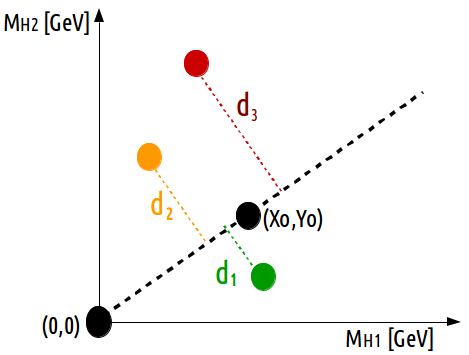
\includegraphics[width=0.5\linewidth]{Figures/AnalysisStrategy/eventselection/pairing/new.png}\\
\end{center}
\vspace{-0.5cm}
\caption[Sketch of the pairing method using the two-dimensional plane of the two reconstructed Higgs boson masses]{Sketch of the pairing method using the two-dimensional plane of the two reconstructed Higgs boson masses (m), where $\hfst$ is leading-$\pt$ di-jet and  $\hsnd$ is subleading-$\pt$ di-jet.}
\label{event_selection:fig:pairing}
\end{figure}

A possible good pairing method is the `closest to the diagonal' or $\dhhfst$-pairing method. In this method, the selected pairing is the one that minimizes the distance from its associated point to the diagonal line passing through the points (0,0) and ($\mathrm{X_{0},Y_{0}}$) using equation~\ref{eq:dhh} (where $\mathrm{k=X_{0}/Y_{0}}$) as illustrated with the green point and $\dhhfst$ distance in Figure~\ref{event_selection:fig:pairing}. By defining k equal to the ratio of the reconstructed Higgs boson average peak positions ($\mathrm{k}=125/120\sim1.04$), the $\dhhfst$-pairing success for the signal benchmarks is the following: 83\% for SM VBF, 89\% for BSM VBF, 82\% SM ggF and 76\% for BSM ggF. 
\begin{equation}
\label{eq:dhh}
\mathrm{ d = \frac{ | \hfstm - k~\hsndm | }{ \sqrt{ 1 + k ^{2} } }}
\end{equation}

The correct pairing properties were studied further in the signal benchmarks in order to improve the $\dhhfst$-based method. The findings are summarized as follows: (1) When the $\dhhfst$-pairing method fails, the correct pairing mostly corresponds to the one with second-closest distance from the associated point to the diagonal line or the $\dhhsnd$-pairing (orange point in Figure~\ref{event_selection:fig:pairing}), (2) the $\dhhfst$-pairing method begins to fail when $|\dhhfst-\dhhsnd|<30$GeV, (3) when the $\dhhfst$-pairing method fails, the reconstructed Higgs tranverse momentum in the center of mass reference frame ($\pt^{*}$(H)) associated to the $\dhhsnd$-pairing tends to be larger than the one from the $\dhhfst$-method. 


From this aforementioned findings, a better pairing algorithm is developed and described as follows: (1) If $\mathrm{|\dhhfst-\dhhsnd|>30~GeV}$, the pairing is obtained from the $\dhhfst$-method (2) otherwise, the pairing is obtained from the method ($\dhhfst$ or $\dhhsnd$) with the largest $\pt^{*}$(H). Figure~\ref{fig:bjetreg} illustrates the distributions of the reconstructed $\hsnd$ and $\hfst$ invariant mass in the SM ggF signal simulation without (blue) and with (red) the application of the b-jet energy regression. The improved pairing success is the following: 91\% for SM VBF, 98\% for BSM VBF, 96\% SM ggF and 82\% BSM ggF. %Furthermore, the pairing method does not sculpt the background events near the signal peak as illustrated later in Figure~\ref{fig:pairingsculpting}.

\begin{figure}[htp!]
\centering
\captionsetup[subfigure]{justification=centering}
\subfloat[]{\centering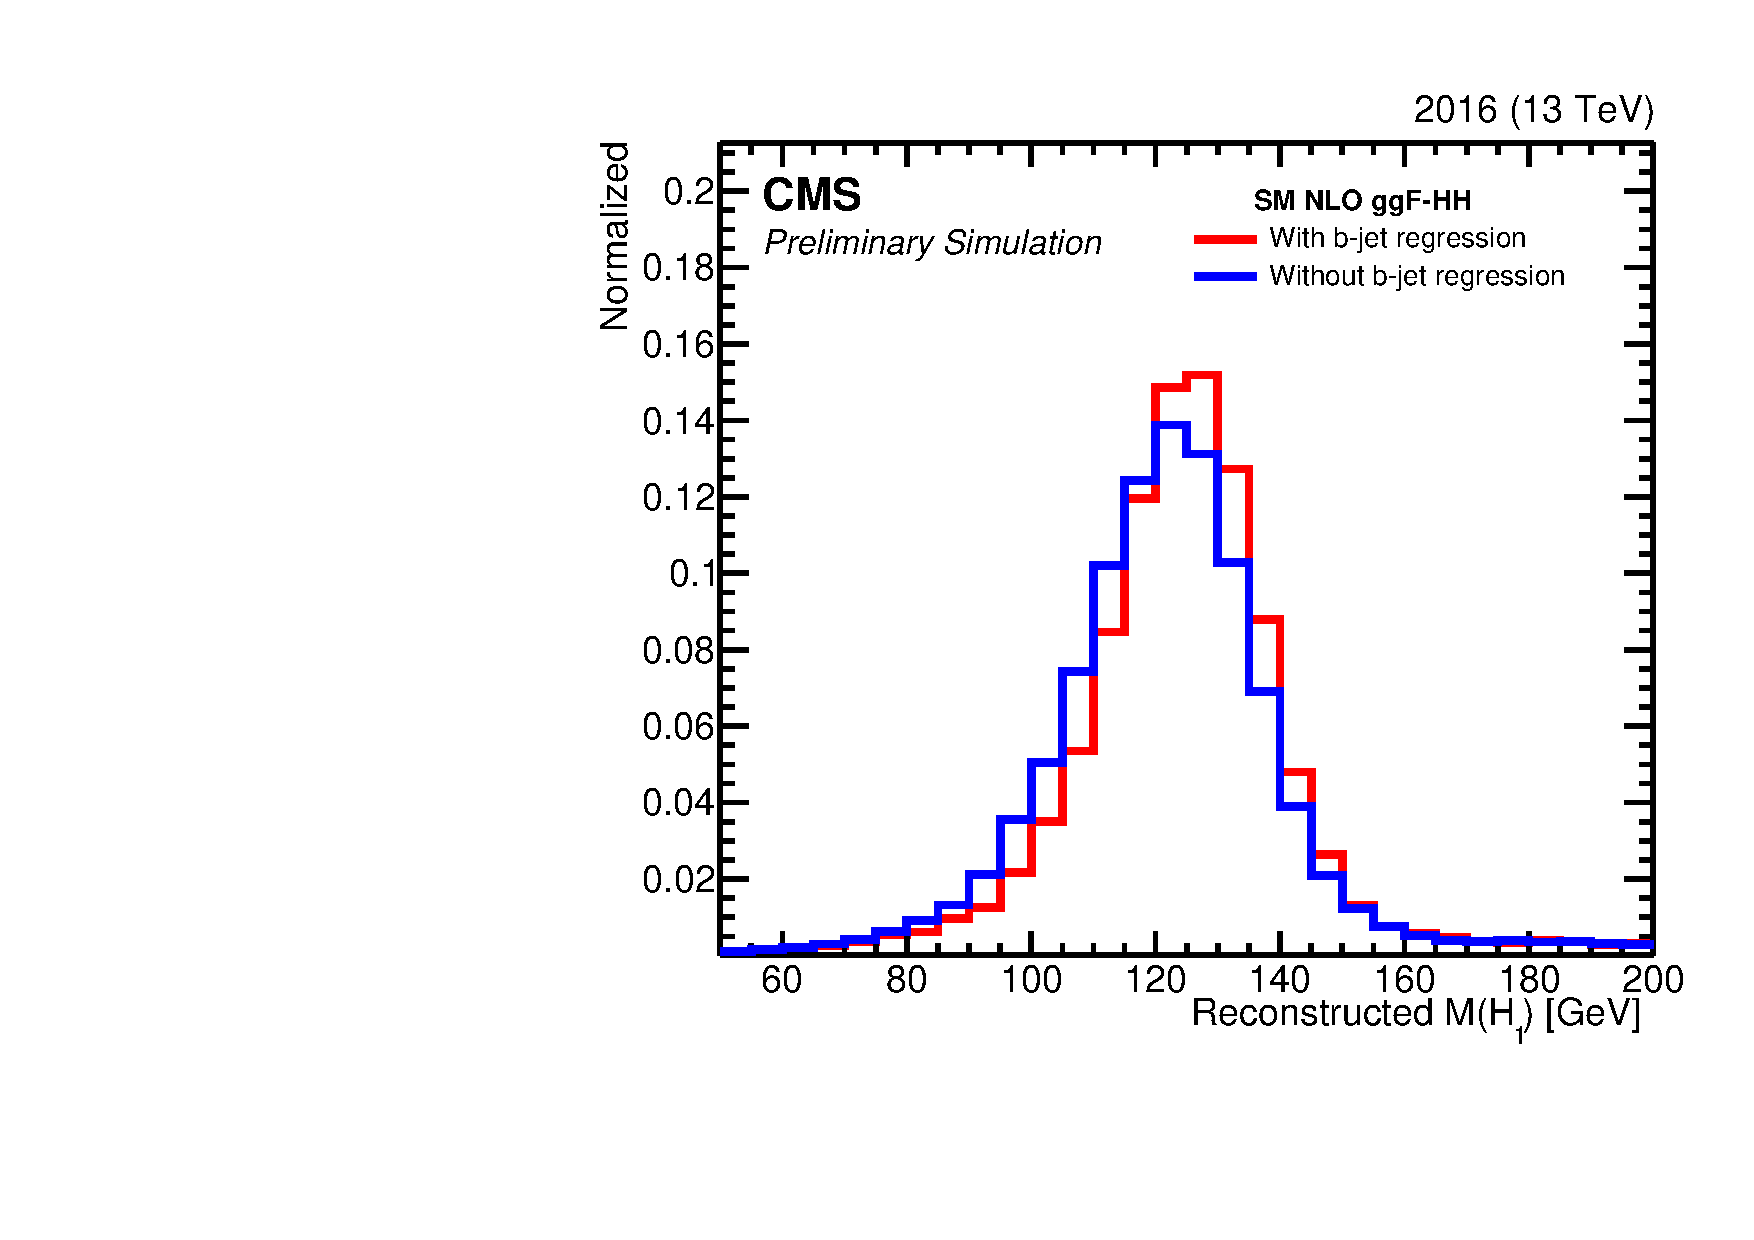
\includegraphics[width=0.5\textwidth]{Figures/AnalysisStrategy/eventselection/bjetenergy/plot_2016_GluGluToHHTo4B_node_cHHH1_TuneCUETP8M1_PSWeights_13TeV-powheg-pythia8_h_H1_m_VS_h_H1unregressed_m.pdf}}
\subfloat[]{\centering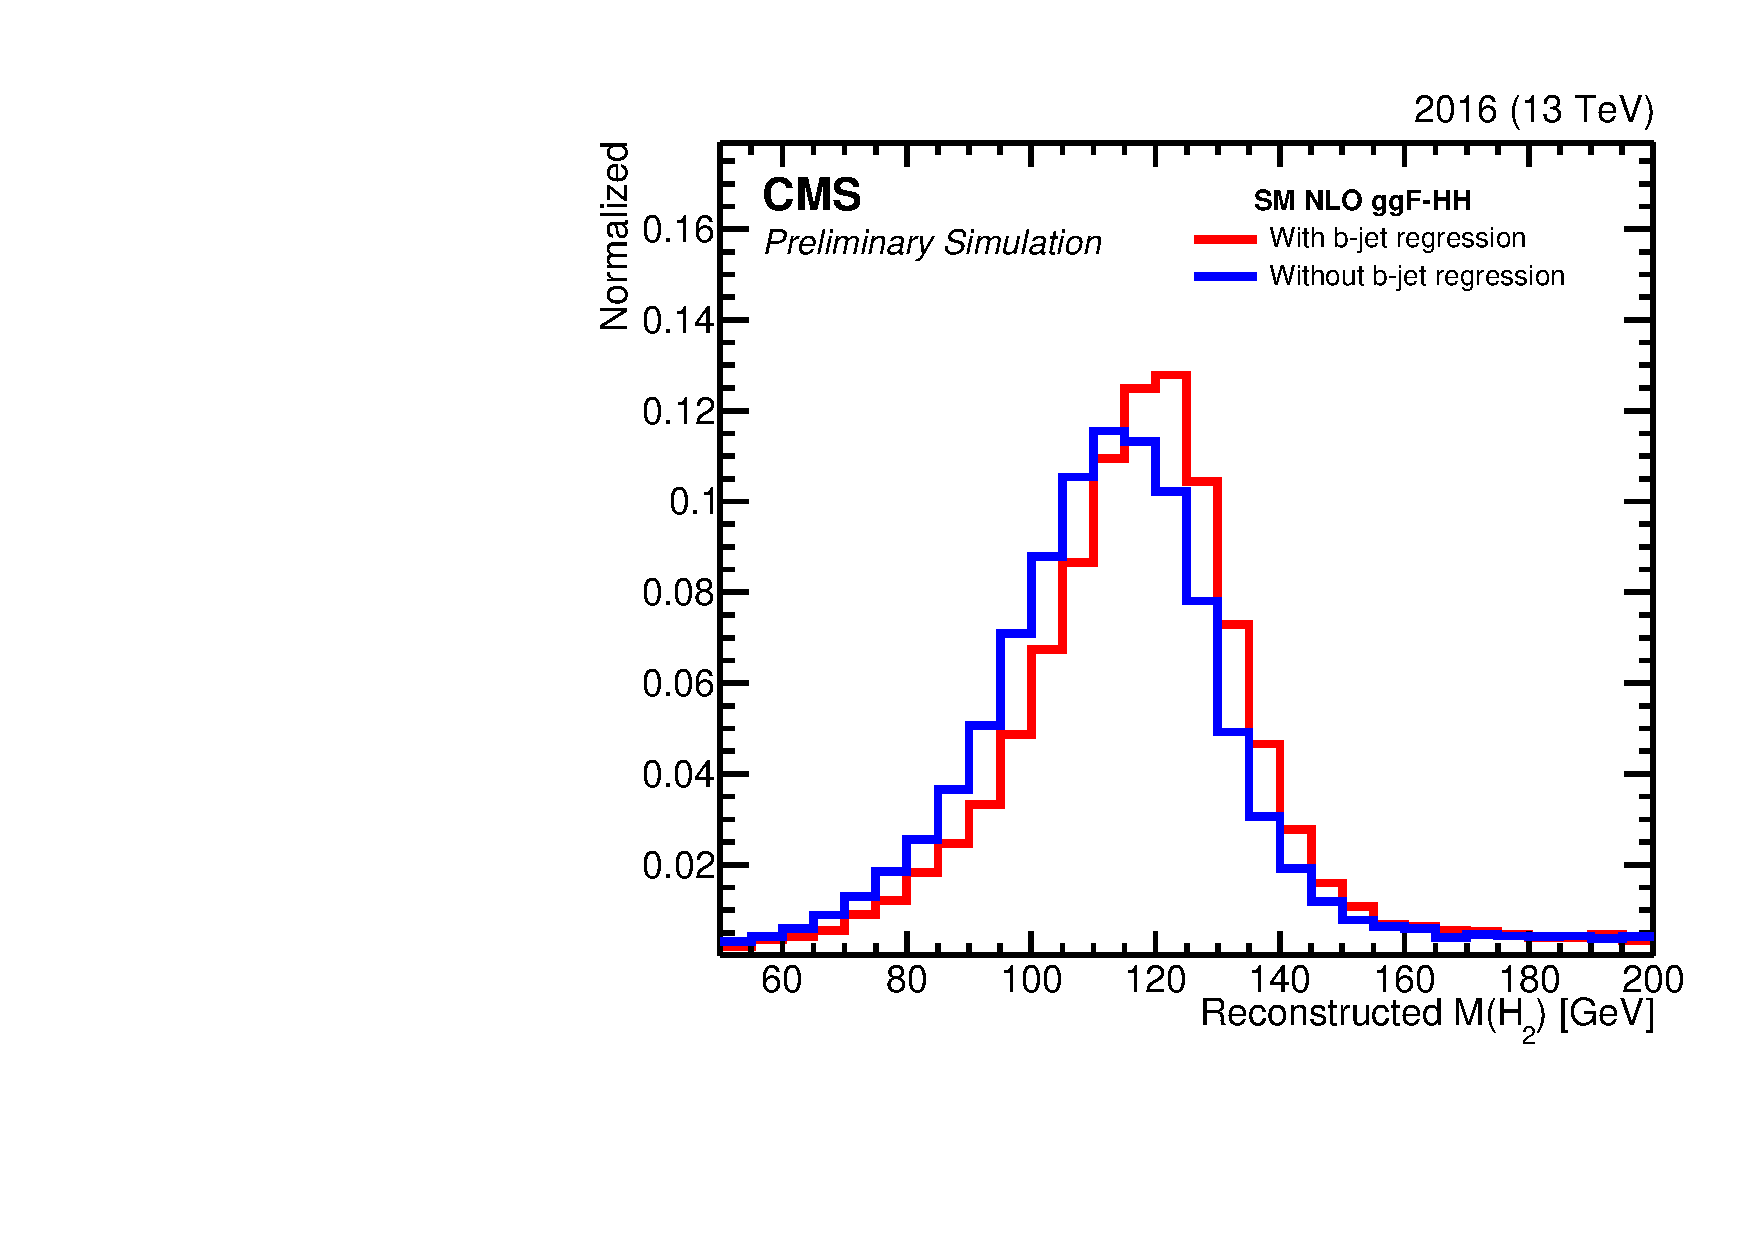
\includegraphics[width=0.5\textwidth]{Figures/AnalysisStrategy/eventselection/bjetenergy/plot_2016_GluGluToHHTo4B_node_cHHH1_TuneCUETP8M1_PSWeights_13TeV-powheg-pythia8_h_H2_m_VS_h_H2unregressed_m.pdf}}
\caption[Invariant mass of the two reconstructed Higgs bosons in SM ggF HH simulated events]{Invariant mass of the two reconstructed Higgs bosons in SM ggF HH simulated events of the 2016 data-taking conditions: A) Highest-$\pt$ di-jet ($\hfst$), B) Lowest-$\pt$ di-jet ($\hsnd$). The distributions are illustrated without (blue) and with (red) the application of the b-jet energy regression.}
\label{fig:bjetreg}
\end{figure}

\subsection{Vector Boson Fusion Jet Pair Candidate} \label{subsec:vbfpair}

To identify whether the HH events are coming from a ggF or a VBF production process, we examine the remaining jets in the collection that have not been selected for the HH reconstruction step to search for the two VBF-jet candidates. The first step is to apply the jet kinematic and quality requirements listed in Table~\ref{event_selection:tab:qjetreq} to obtain the list of VBF jet candidates.

It is important to mention that during 2017 data collection was observed a large ECAL Endcap (EE) noise in the forward region. This EE noise increased the jet multiplicity with `noise-jets' characterized by a raw $\pt<50$ GeV and $2.6<|\eta|<3.1$. In the 2017 preselection, we require the tightest working point of the PUID algorithm on jets located at that $\eta$ region.

\begin{table}[htb]
\caption[Summary of jet kinematic and quality requirements for VBF-jet candidates]{\label{event_selection:tab:qjetreq} Summary of jet kinematic and quality requirements for VBF-jet candidates. The PileupID requirement is only applied to jets with $\pt<50$ GeV.}
\centering
\begin{tabularx}{\textwidth}{XXXXX}
	\hline
	Dataset & $\pt$ [GeV] &$|\eta|$  & PileupID & JetID\\ 
	\hline
	2016    & $>25$        & $<4.7$  & Medium   & Tight\\ 
	2017    & $>25$        & $<4.7$  & Medium   & Tight\\ 
	2018    & $>25$        & $<4.7$  & Medium   & Tight\\
	\hline
\end{tabularx}
\end{table}

Simulation studies show that preselected VBF signal events with at least two VBF jet candidates (where the four b quarks from the HH decay and the two outgoing patrons from the VBF process are all reconstructed as six jets) have the following properties: (1) The VBF outgoing partons (q1 and q2) have opposite $\eta$-sign  ($\mathrm{\eta_{q1}~x~\eta_{q2}<0}$) in 94-98\% of the cases depending on c2v coupling, and (2) the highest-$\pt$ VBF-jet candidate is one of the real VBF jets in ~93-94\% of the cases. Based on this information, the VBF-jet candidate with the highest-$\pt$ is chosen as the highest-$\pt$ VBF jet (j1). Then, we check all the opposite $\eta$-sign VBF-jet candidates to select the lowest-$\pt$ VBF-jet (j2). If multiple jets with opposite $\eta$-sign jet are found (around 30\% of the time), then the one with the largest $\pt$ is chosen to be j2. It is important to mention here that we tested different ways to make the j2-choice: largest $\pt$ (nominal), largest VBF pair pseudorapidity separation, largest VBF pair mass. We found that the three options have similar VBF purity as seen in Figure~\ref{fig:vbfj2purity} for VBF signal with $\kvv=2$. However, we expect that nominal choice to have better signal and background separation because it would not sculpt the distributions of $\mathrm{m_{j1j2}}$ and $\Delta\eta$(j1,j2) at high values (signal-enriched regions). 

Preselected events with a fully reconstructed VBF-jet pair are classified to the `Pre-VBF' region and denominated as `pre-VBF' events, otherwise are denominated classified to the `Pre-ggF' region and denominated as `pre-ggF' events. The event yields in data and MC simulated events is presented in Table~\ref{event_selection:tab:presel}.

\begin{figure}[htb]
\begin{center}
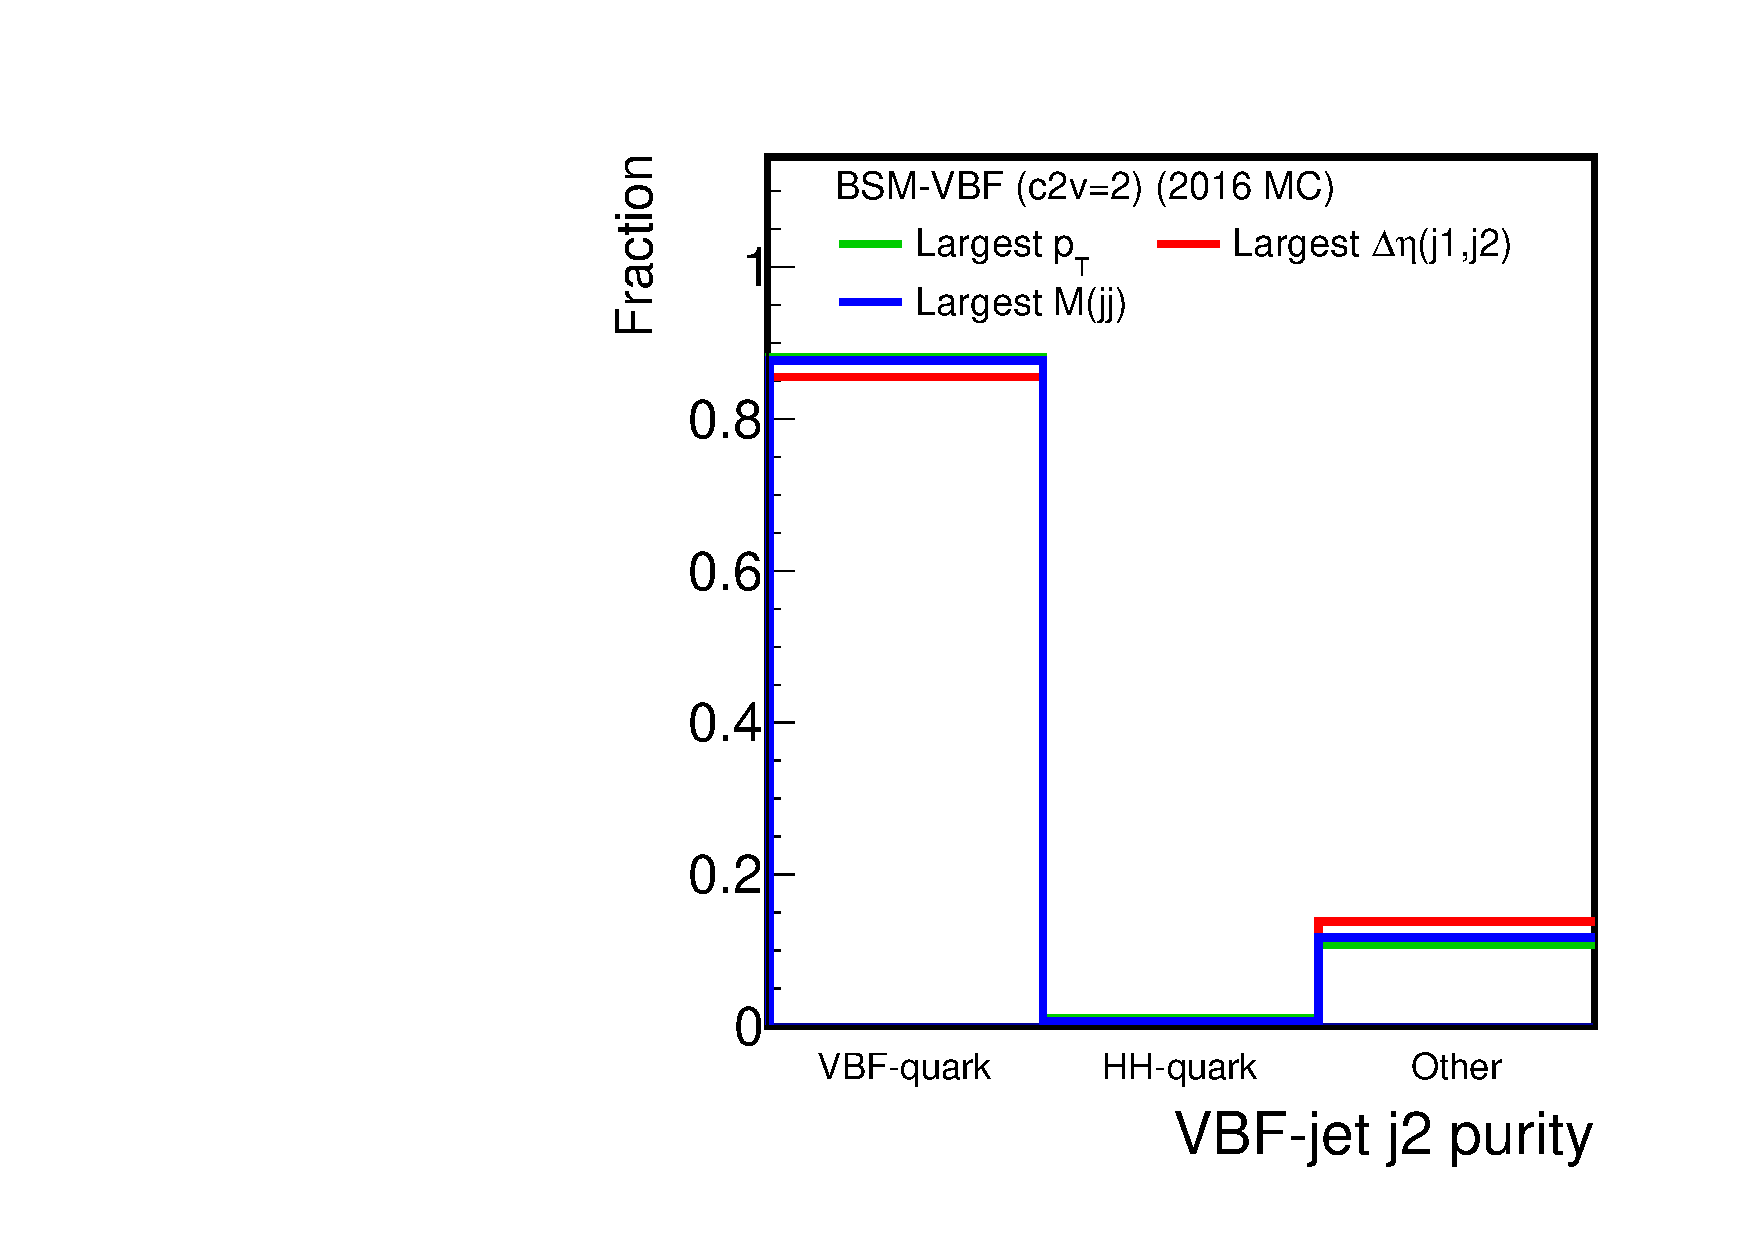
\includegraphics[width=0.50\linewidth]{Figures/AnalysisStrategy/eventselection/pairing/purityBSMvbf2016.pdf}\\
\end{center}
\vspace{-0.5cm}
\caption[Purity of the lowest tranverse momentum VBF jet candidate]{Purity of the lowest transverse momentum VBF jet candidate (j2) using three different methods in events with multiple opposite $\eta$-sign jets: (green) largest $\pt$, (red) largest VBF pair pseudorapidity separation, (blue) largest VBF pair mass. The simulated events correspond to VBF signal with $\kvv=2$ in the 2016 data-taking conditions.}
\label{fig:vbfj2purity}
\end{figure}

\begin{table}[htb]
\caption[Event yields of data and MC simulation after preselection requirements]{\label{event_selection:tab:presel} Event yields of data and MC simulation after preselection requirements. The processes ggF, VBF and VBF$(\kvv=2)$ are multiplied by a factor of $10^{2}$.}
\centering
\begin{tabularx}{\textwidth}{lrrrrrr}
	\hline
	Dataset/Presel.           & 2016/ggF  & 2016/VBF & 2017/ggF  & 2017/VBF & 2018/ggF & 2018/VBF \\
	\hline
    ggF                       &   1174.3 &  443.0  &    763.9 &  270.6  &   1338.9 &  527.1  \\ 
    VBF                       &      8.8 &   18.4  &      6.6 &   12.2  &     11.8 &   25.1  \\ 
    VBF ($\kvv=2$)            &    607.7 &  976.3  &    444.9 &  580.3  &    910.7 &  1300.8 \\ 
    QCD multijet              & 121147.7 & 52818.2 &  52149.2 & 25017.0 &  86381.0 & 39741.9 \\ 
    $\ttbar$                  &   4614.0 &  6761.0 &   2611.5 &  3973.1 &   5369.2 &  8648.7 \\ 
    Single Higgs              &    296.4 &  441.7  &    208.1 &  302.1  &    392.4 &  601.4  \\ 
    ZZ$\rightarrow$4b         &     30.5 &   7.1   &     17.3 &   4.7   &     29.9 &   8.7   \\  
    Total MC Bkg.             & 126088.6 & 60028.0 &  54986.1 & 29296.9 &  92172.5 & 49000.7 \\ 
    Data                      & 153170 & 69702 & 110500 & 57594 & 164307 & 96274 \\ 
	\hline
\end{tabularx}
\end{table}

\clearpage
\section{Event Categorization} \label{sec:categories} 
\subsection{Motivation}
The HH search aims at having production mode (ggF and VBF) event categories with the highest signal purity possible to maximize the measurement of both the ggF and VBF signals.  As observed in Table~\ref{event_selection:tab:presel}, there is about 26-28\% of the SM ggF signal events are classified in the pre-VBF event region. Furthermore, the ratio between the SM ggF and SM VBF signals in Pre-VBF events is approximately 21.0-24.1, and the ratio between SM ggF and VBF (c2v=2) signals in pre-VBF events is 0.41-0.47. Consequently, pre-ggF and pre-VBF regions do not have a good production mode purity. As a next step, the strategy is to use a production mode discriminant or score, to reduce ggF signal assigned to the pre-VBF event region and re-assign it back to the ggF signal-enriched region, thus creating higher purity ggF and VBF categories. 

\subsection{Production Mode Score: ggFKiller} \label{subsection:ggfkiller}
The production mode score discussed above is named `ggFKiller'. It is trained and used in the kinematic phase space of the pre-VBF region. The ggFKiller aims to maximize the following: (1) the efficiency of the assignment of SM ggF signal events to the ggF signal-enriched region, (2) the sensitivity to measure both SM VBF signal and VBF signal with anomalous $\kvv$ couplings. 

The chosen multivariate analysis (MVA) algorithm is a Boosted Decision Tree (BDT) implemented in the XGBoost package~\cite{xgboost}. The VBF signal with the $\kvv = 2$ and SM ggF signal models are defined as the `signal' events and `background' events in the training, respectively. The specific choice of $\kvv$ is motivated by the largest BSM kinematic enhancement among the available VBF signal simulated samples.  The ggFKiller is built using 14 kinematic variables and correlations among the reconstructed Higgs bosons and the VBF-jets. The list of variables is presented in Table~\ref{tab:ggfkillervars}. Three independent trainings are performed depending on the simulation year. For illustration, the signal (VBF with $\kvv=2$) and background (SM ggF) input variable distributions of the 2016 simulated data-taking conditions are presented in Figure~\ref{event_selection:fig:bdtvariables2016}. More information regarding the ggFKiller training and optimization is presented in Appendix~\ref{appendix:ggfkiller}.

\clearpage

\begin{figure}[htbp!]
\begin{center}
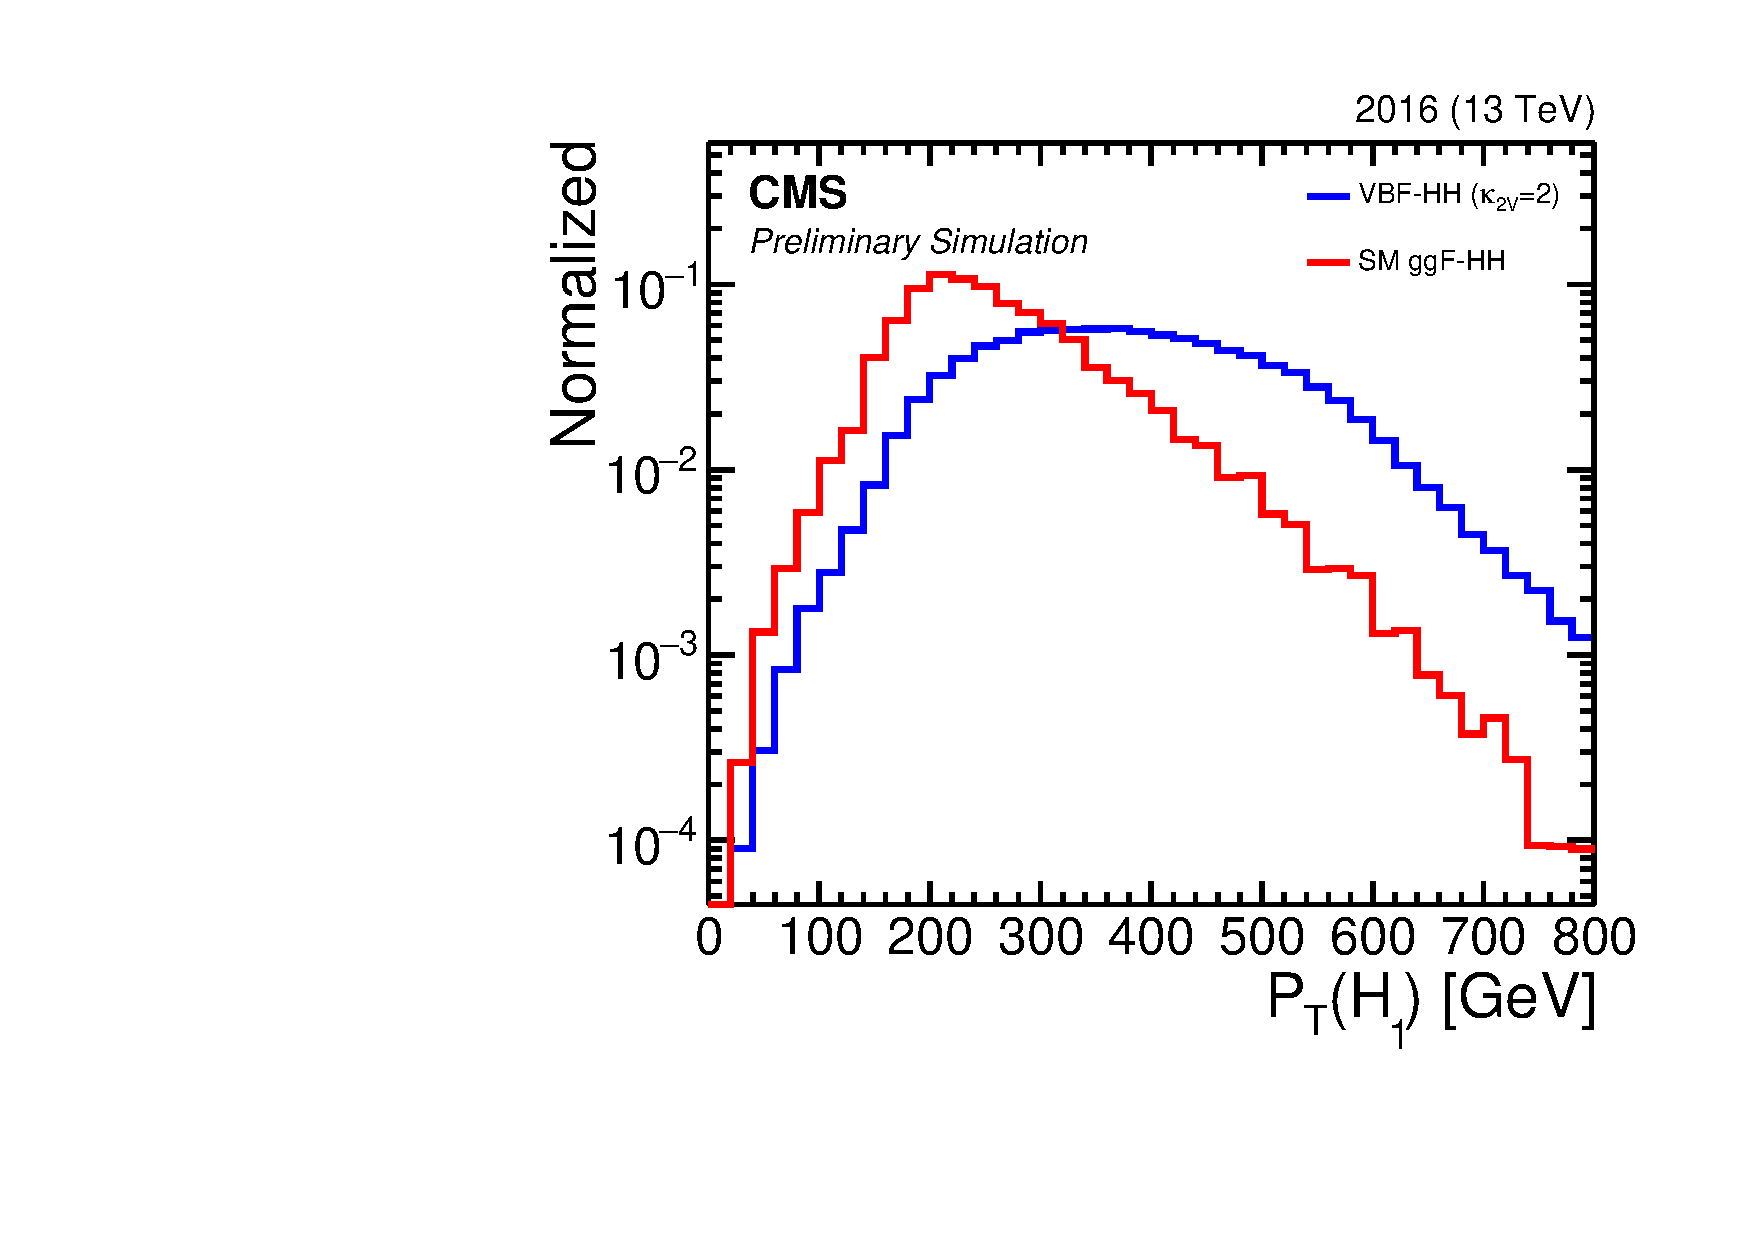
\includegraphics[width=0.27\linewidth]{Figures/AnalysisStrategy/eventselection/ggfkiller/2016ggfkiller/plot_2016_h_H1_pt.pdf}
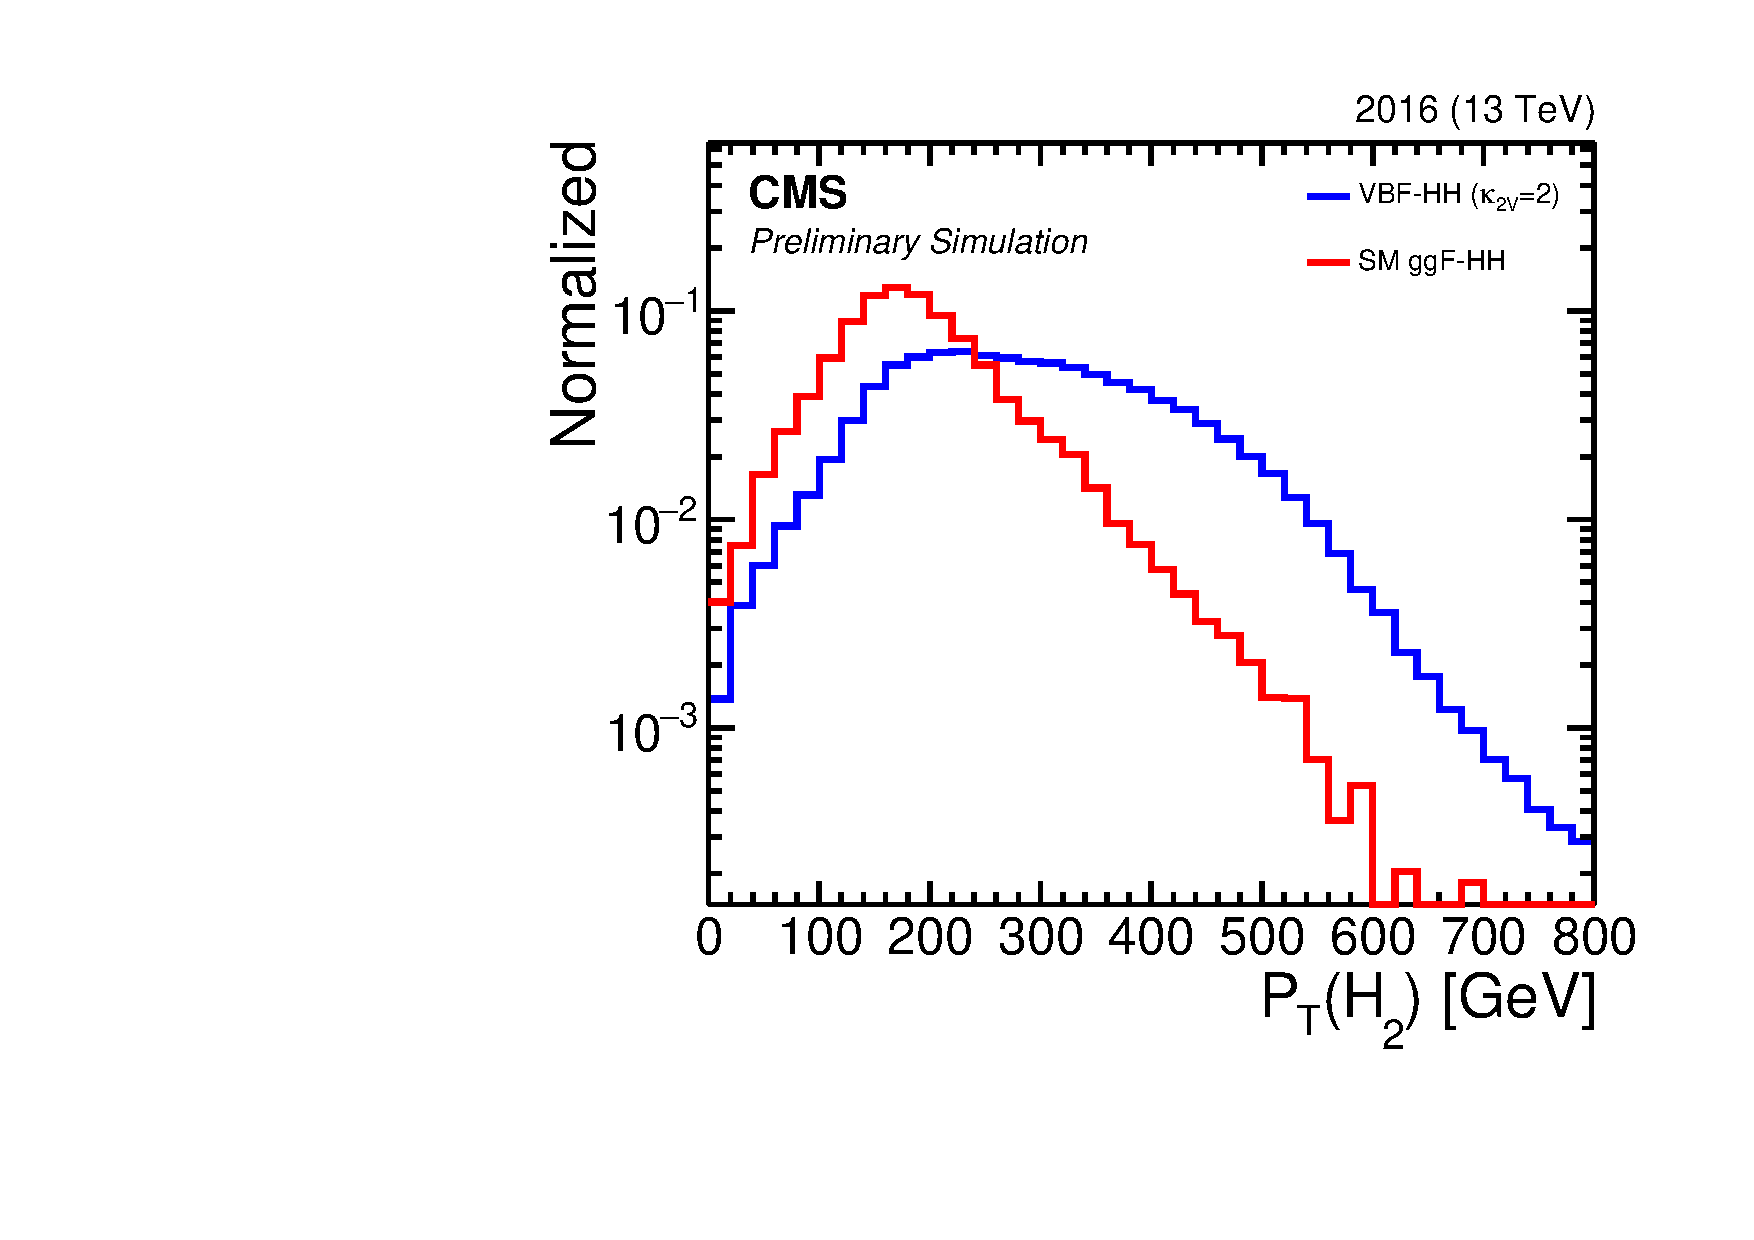
\includegraphics[width=0.27\linewidth]{Figures/AnalysisStrategy/eventselection/ggfkiller/2016ggfkiller/plot_2016_h_H2_pt.pdf}
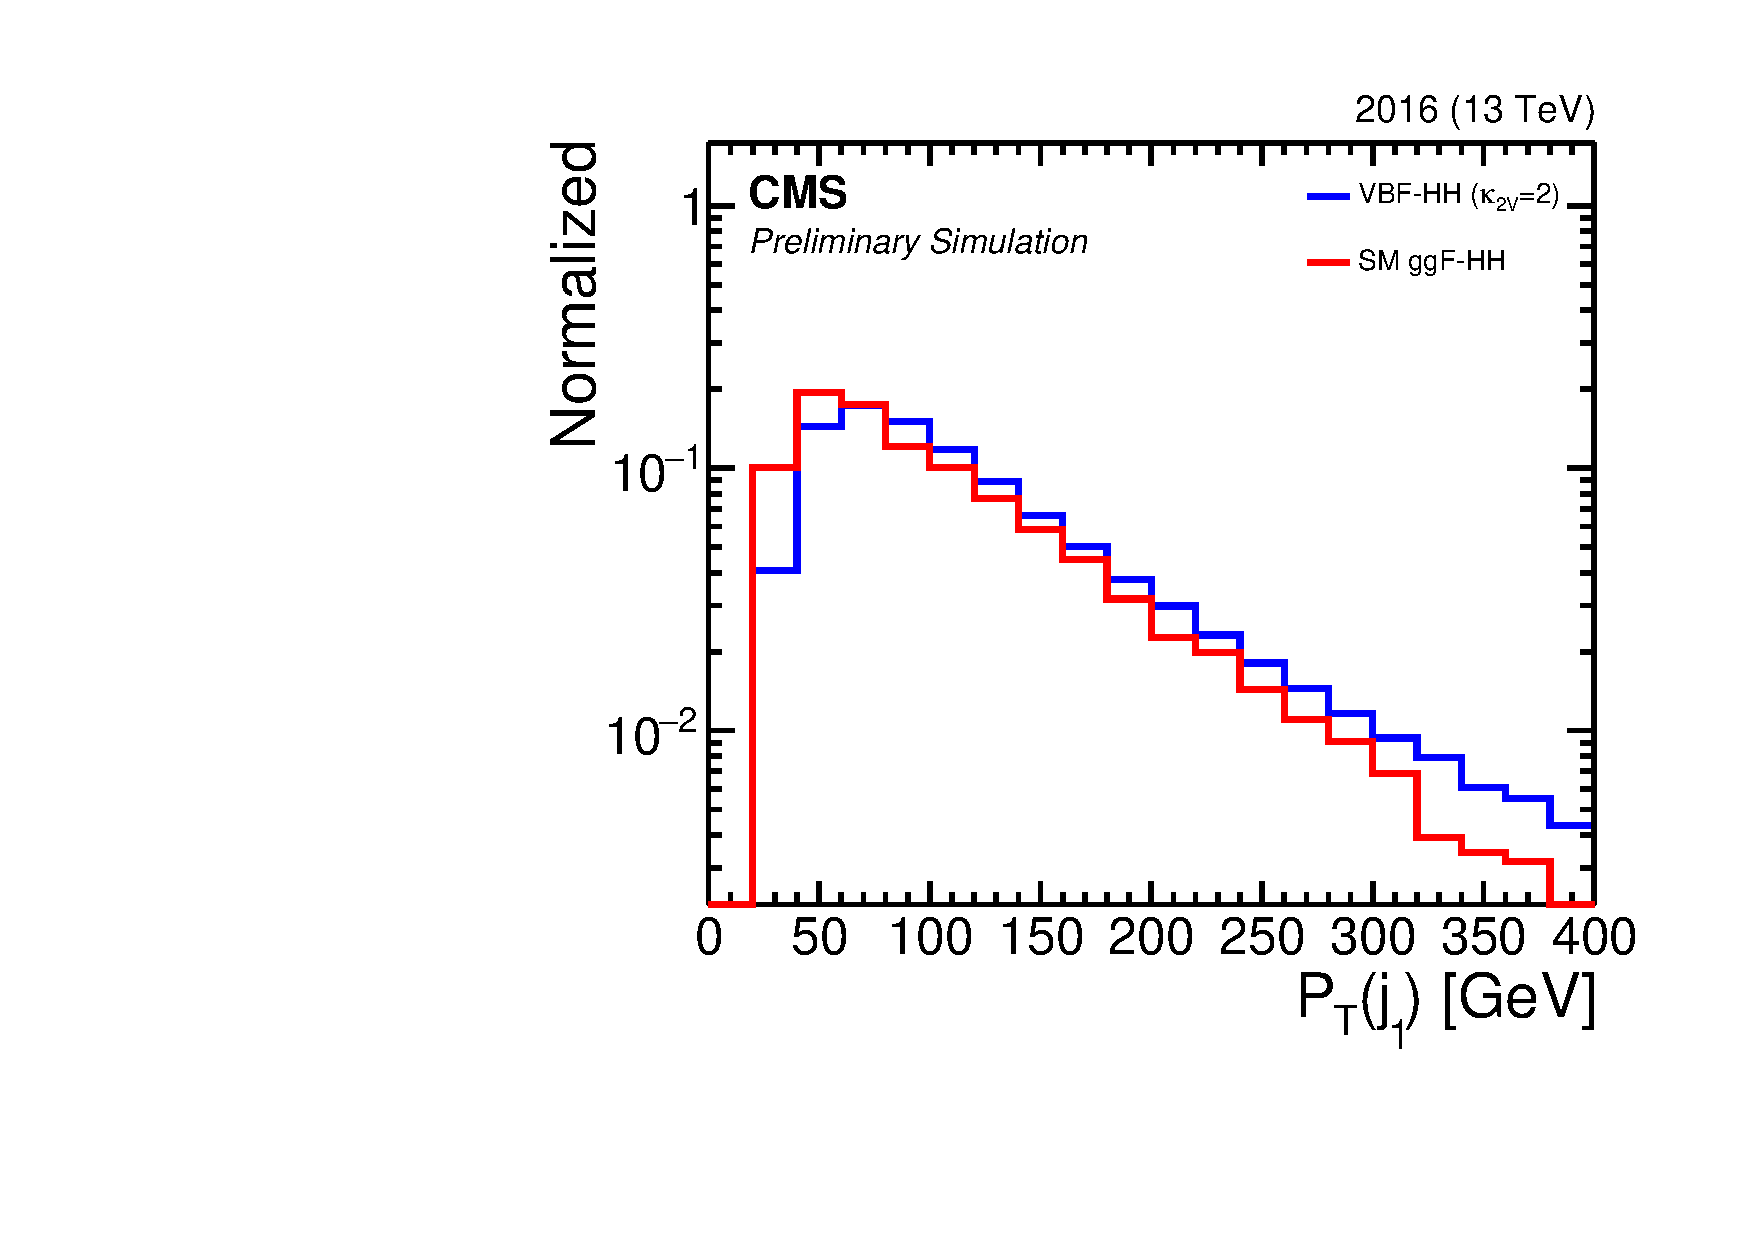
\includegraphics[width=0.27\linewidth]{Figures/AnalysisStrategy/eventselection/ggfkiller/2016ggfkiller/plot_2016_h_JJ_j1_pt.pdf} \\
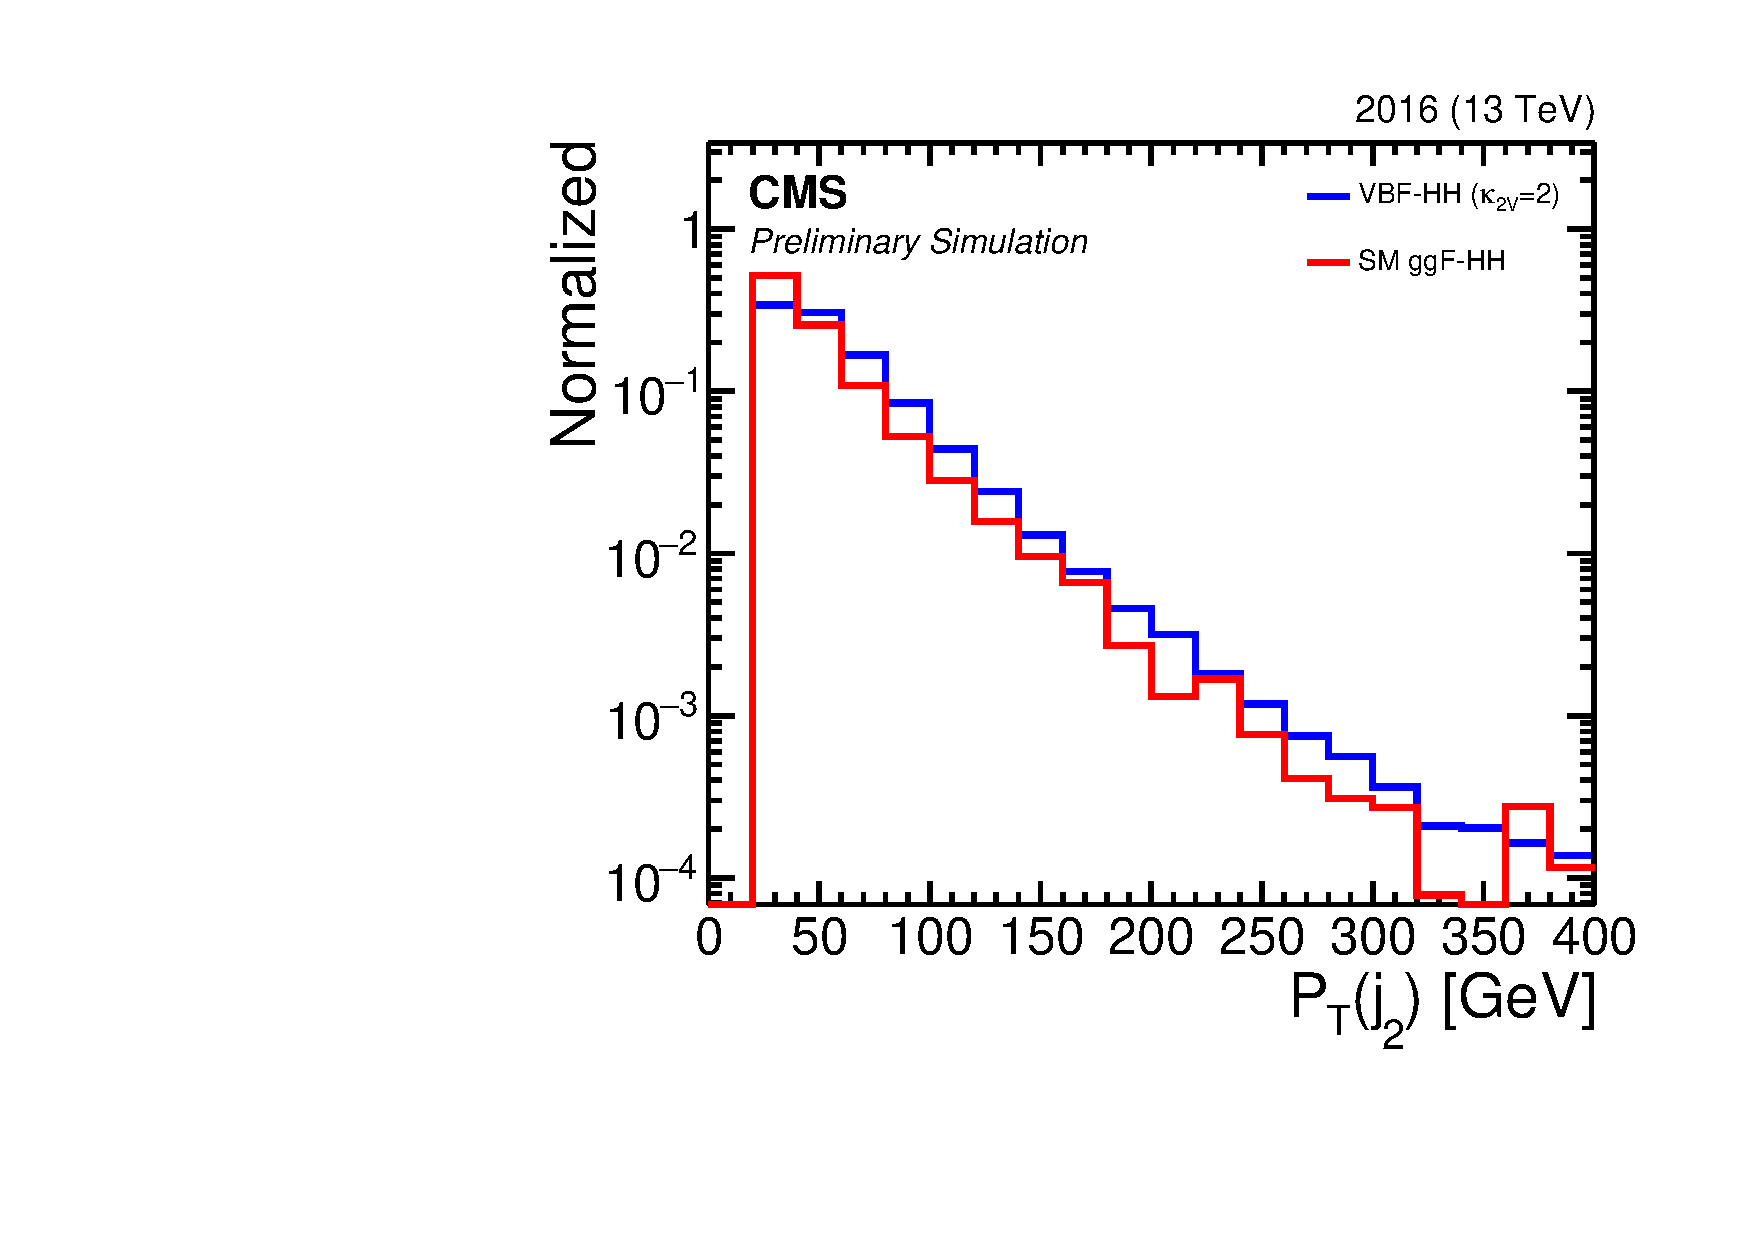
\includegraphics[width=0.27\linewidth]{Figures/AnalysisStrategy/eventselection/ggfkiller/2016ggfkiller/plot_2016_h_JJ_j2_pt.pdf}
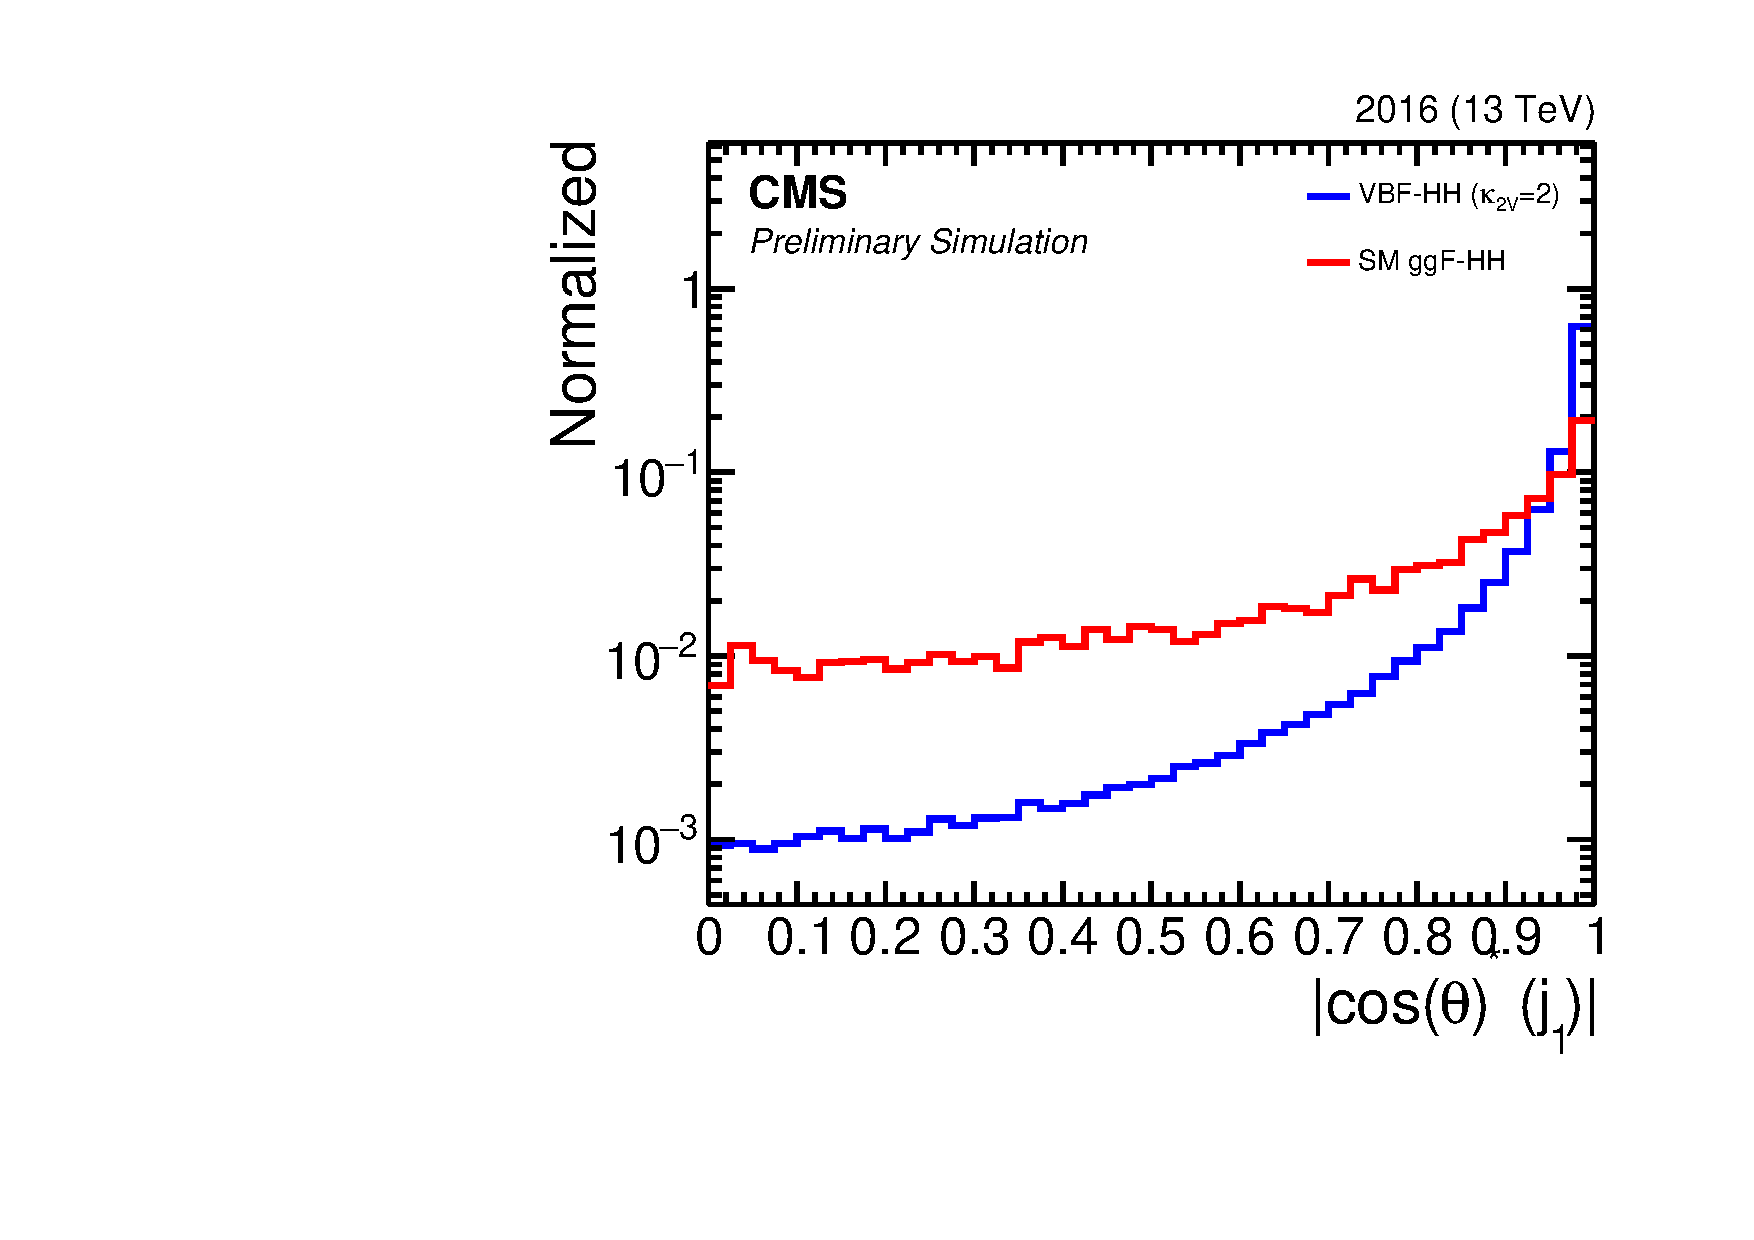
\includegraphics[width=0.27\linewidth]{Figures/AnalysisStrategy/eventselection/ggfkiller/2016ggfkiller/plot_2016_h_abs_costh_JJ_j1_vbfcm.pdf}
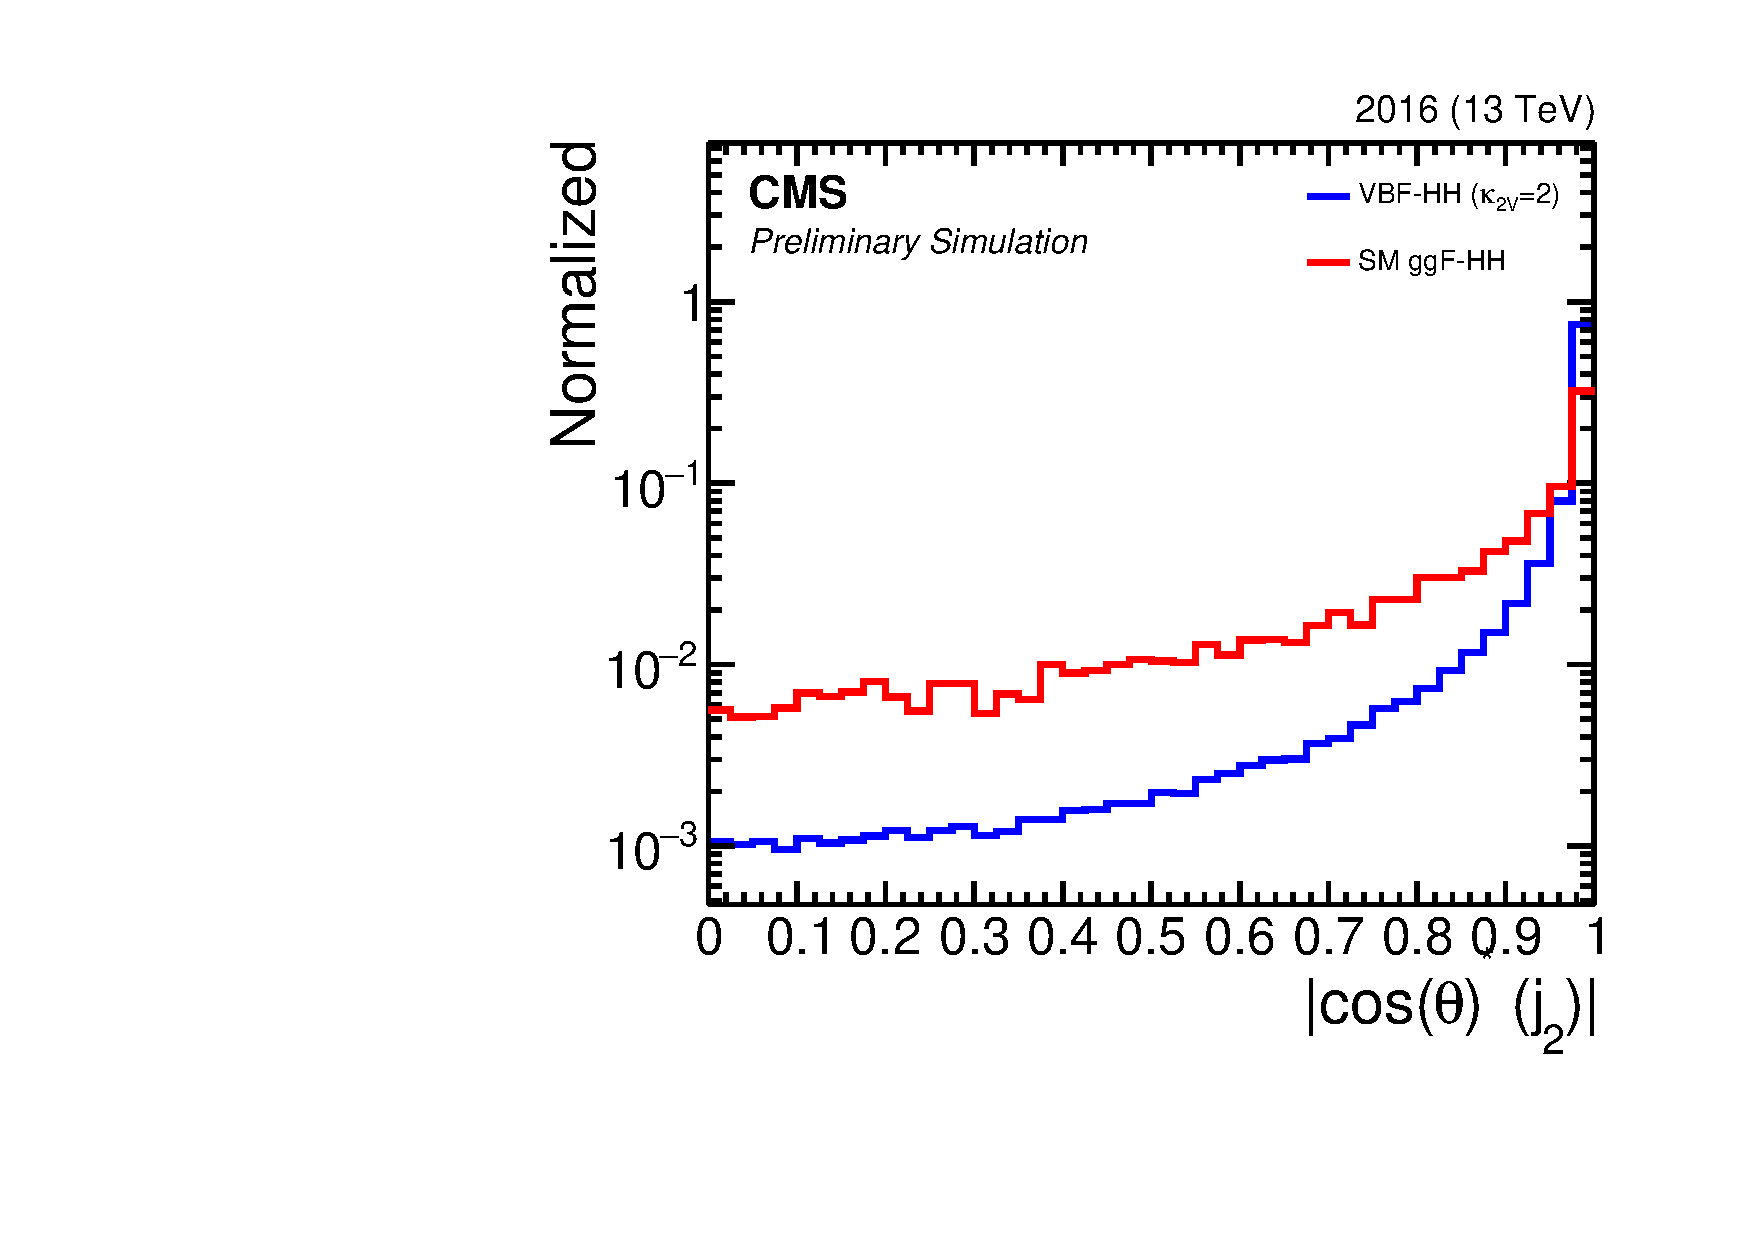
\includegraphics[width=0.27\linewidth]{Figures/AnalysisStrategy/eventselection/ggfkiller/2016ggfkiller/plot_2016_h_abs_costh_JJ_j2_vbfcm.pdf}
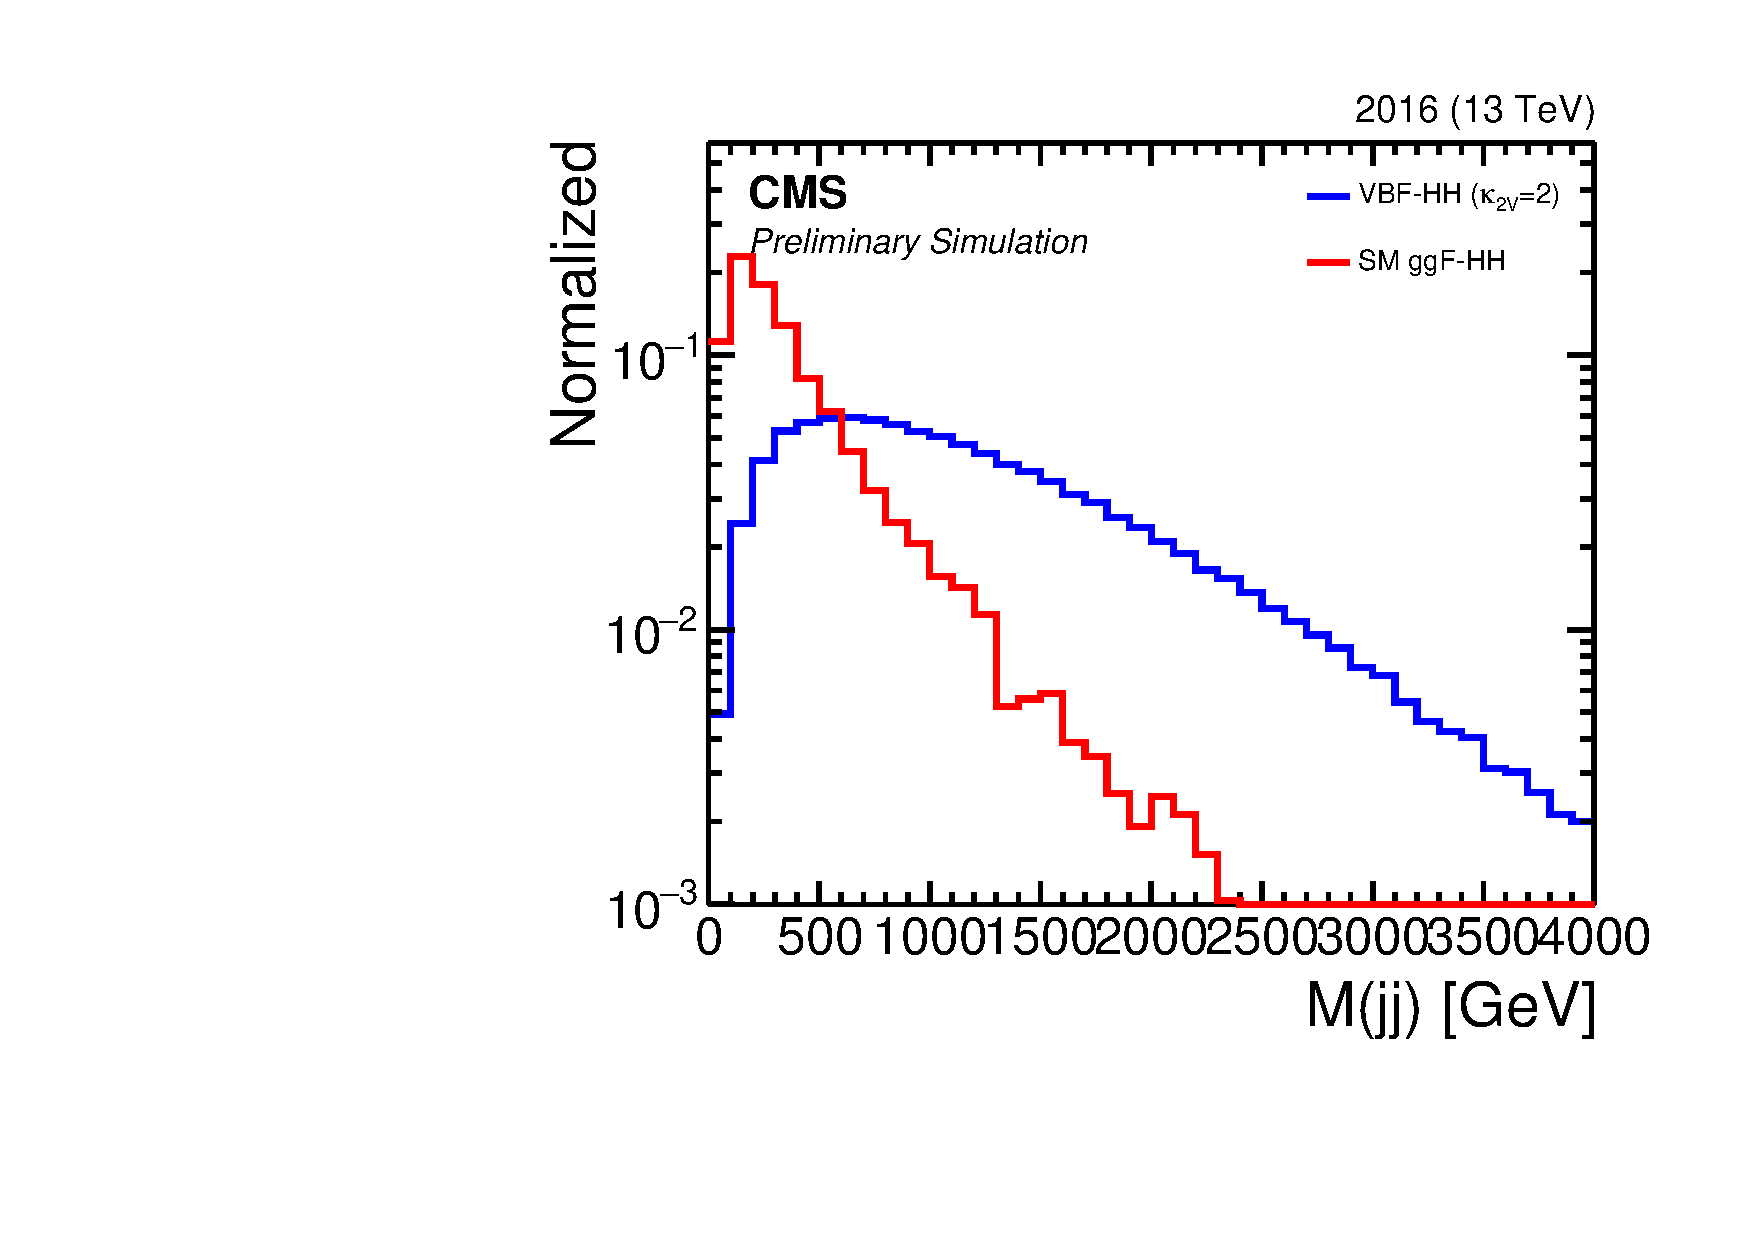
\includegraphics[width=0.27\linewidth]{Figures/AnalysisStrategy/eventselection/ggfkiller/2016ggfkiller/plot_2016_h_JJ_m.pdf}
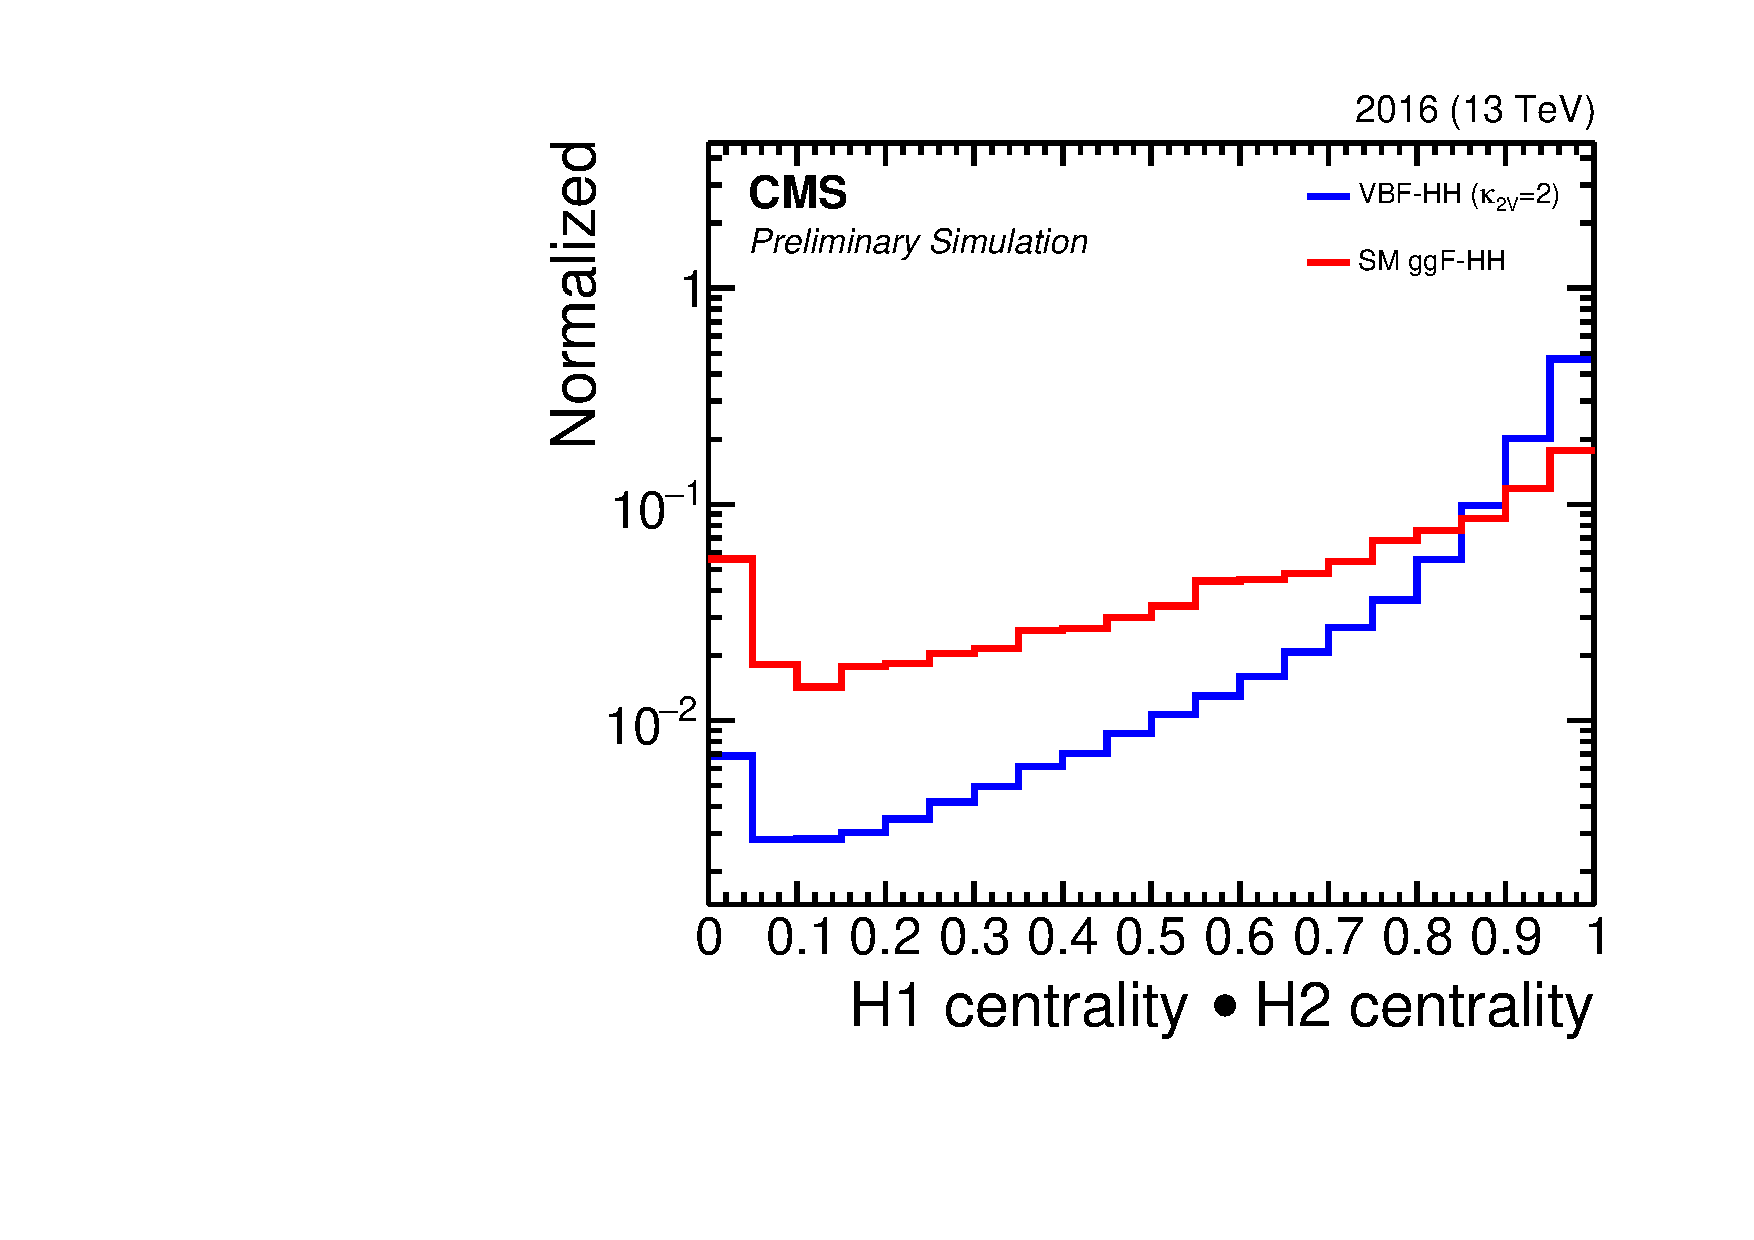
\includegraphics[width=0.27\linewidth]{Figures/AnalysisStrategy/eventselection/ggfkiller/2016ggfkiller/plot_2016_h_H1H2_centrality.pdf}
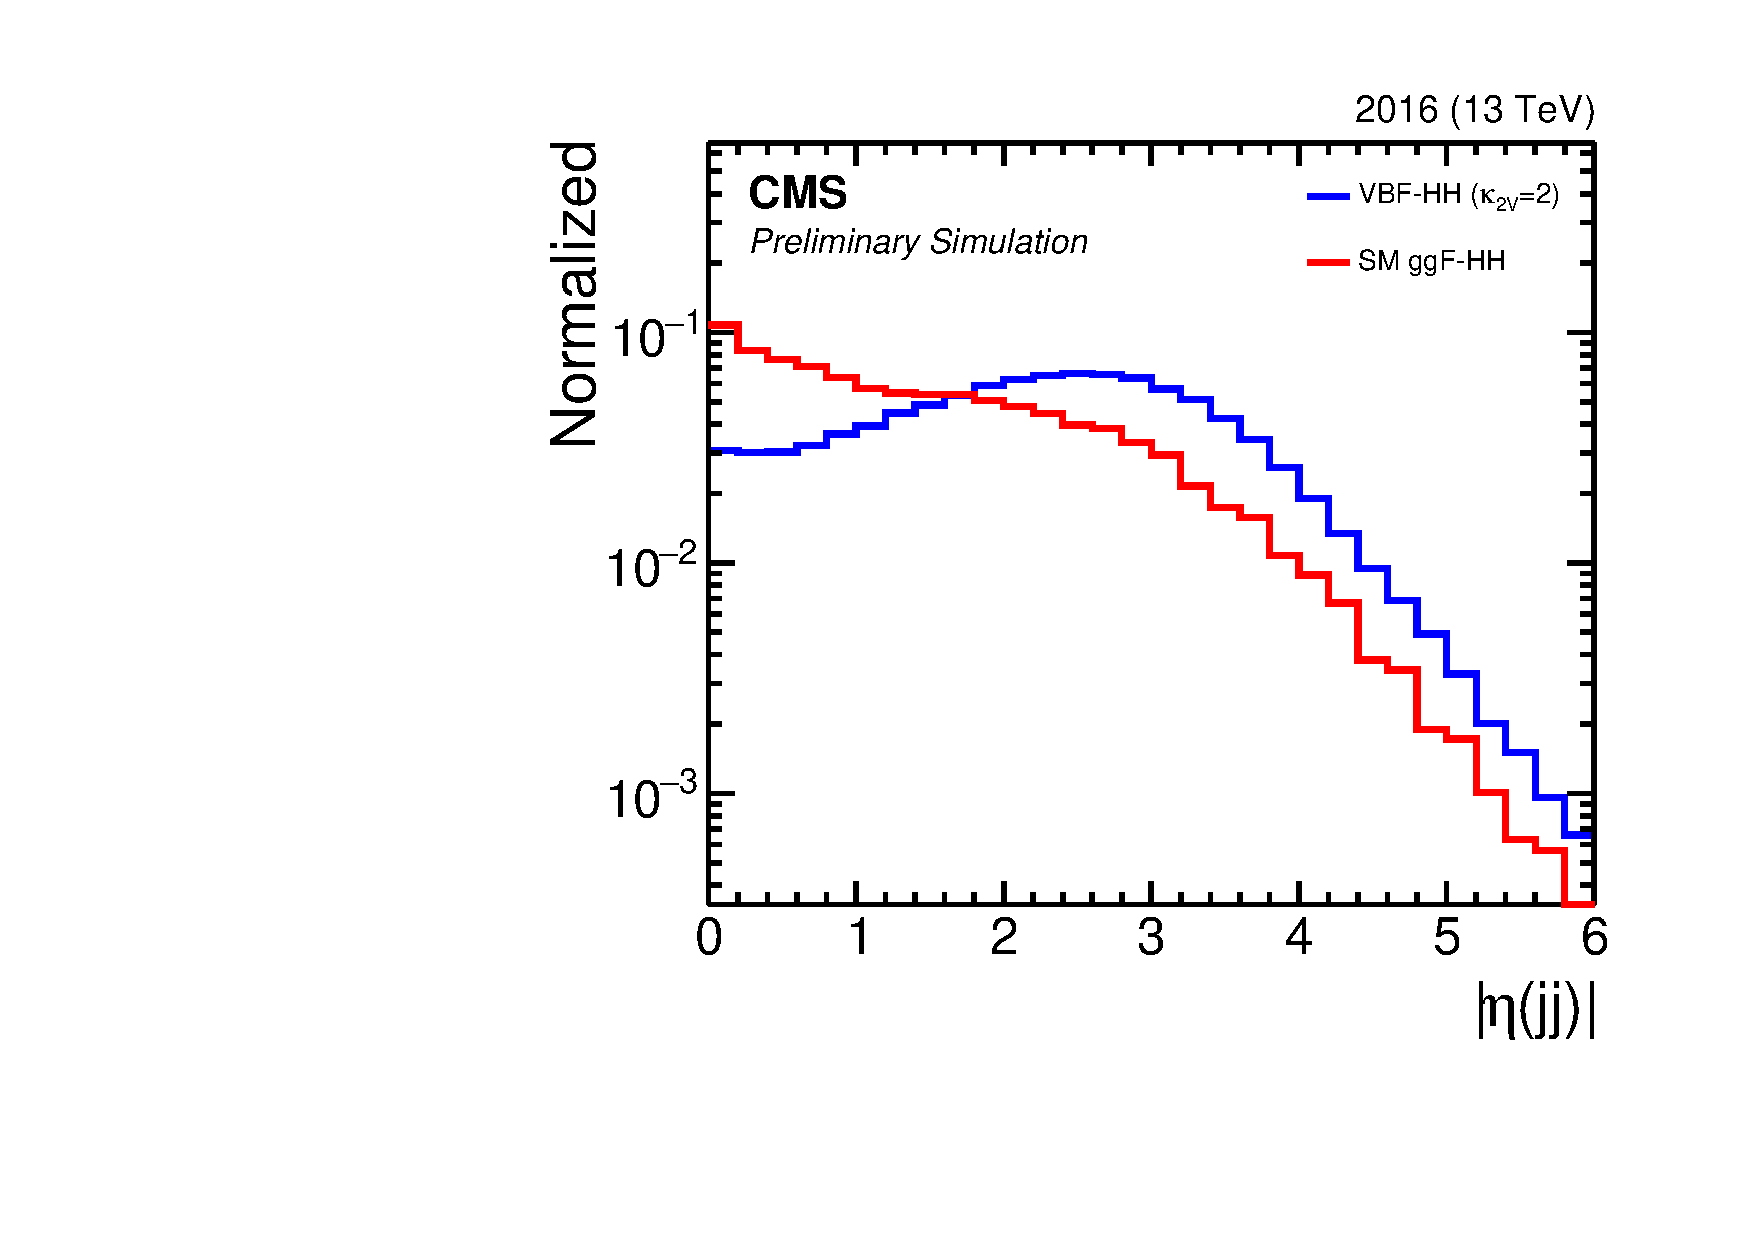
\includegraphics[width=0.27\linewidth]{Figures/AnalysisStrategy/eventselection/ggfkiller/2016ggfkiller/plot_2016_h_JJ_eta.pdf}\\
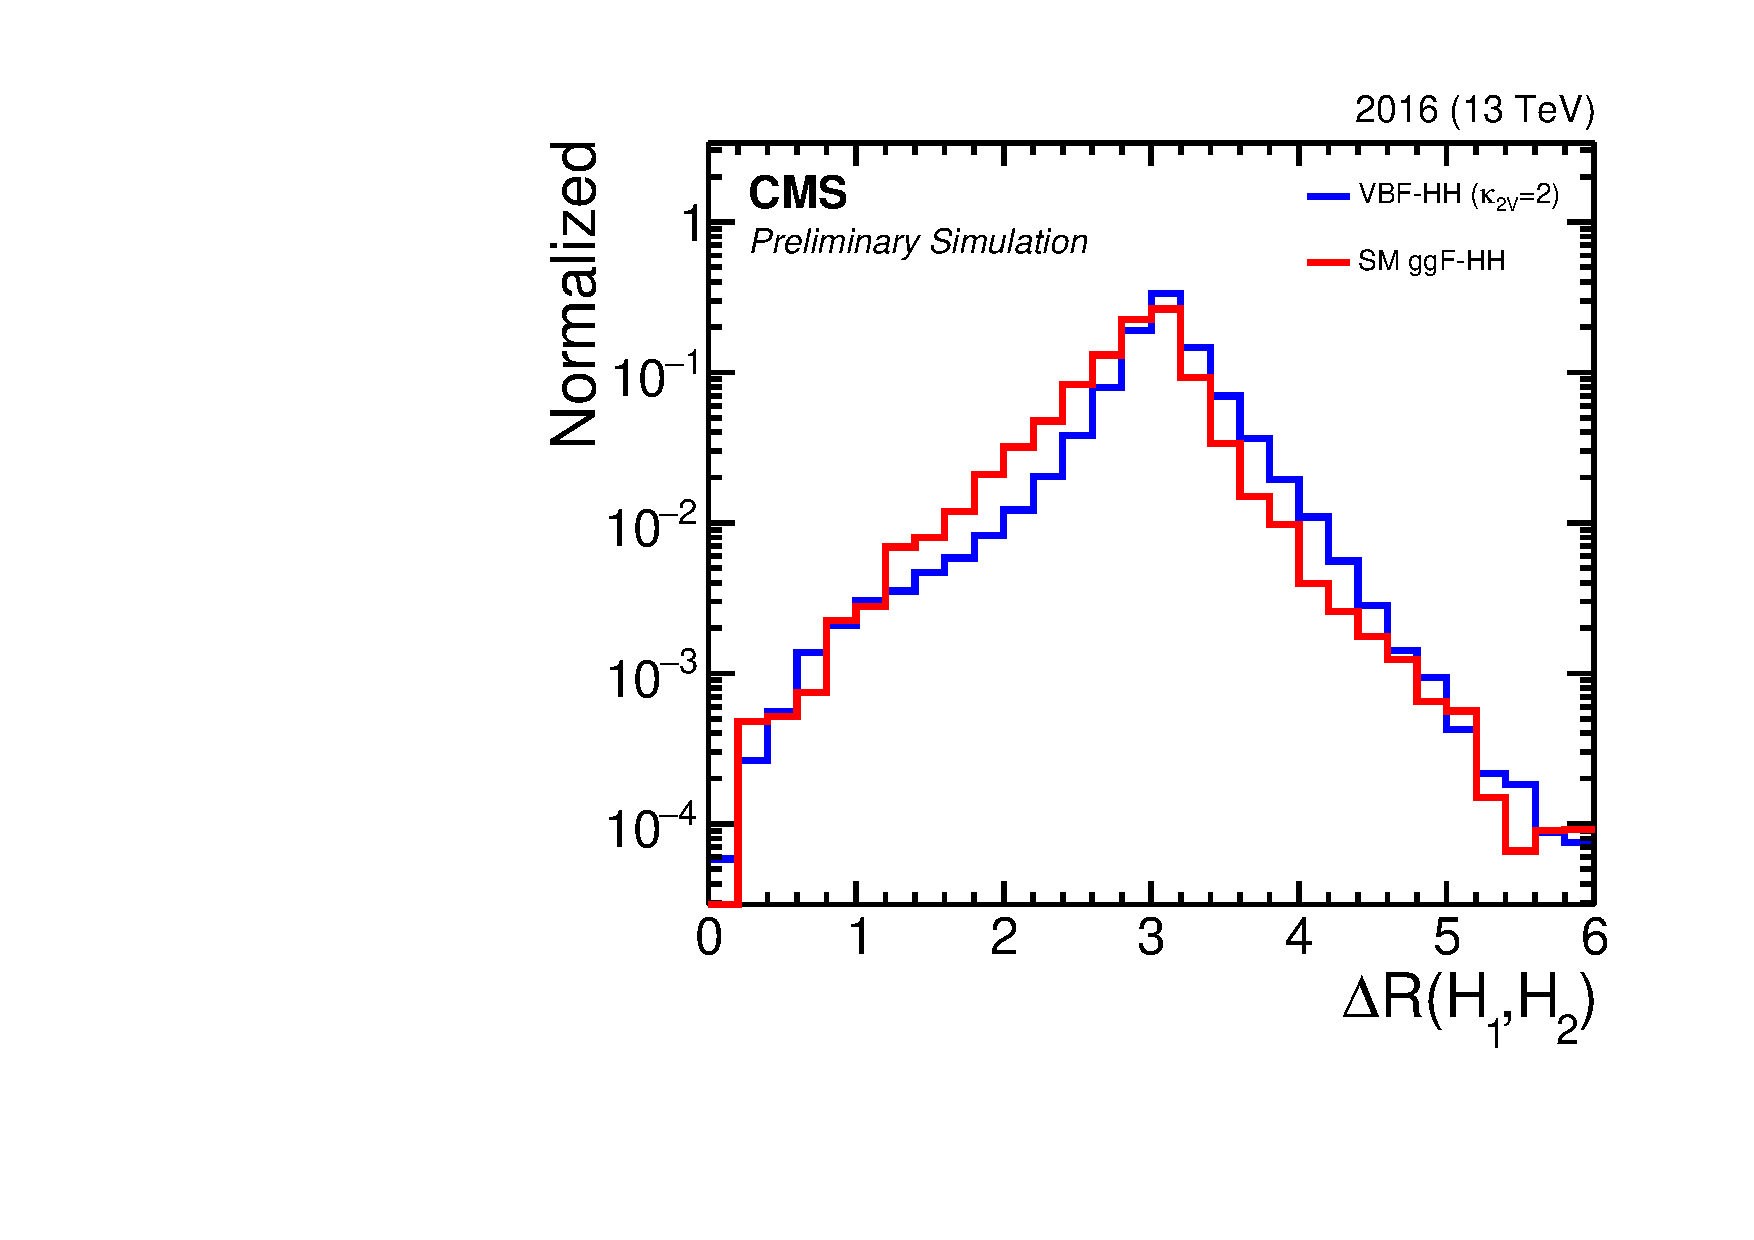
\includegraphics[width=0.27\linewidth]{Figures/AnalysisStrategy/eventselection/ggfkiller/2016ggfkiller/plot_2016_h_h1h2_deltaR.pdf}
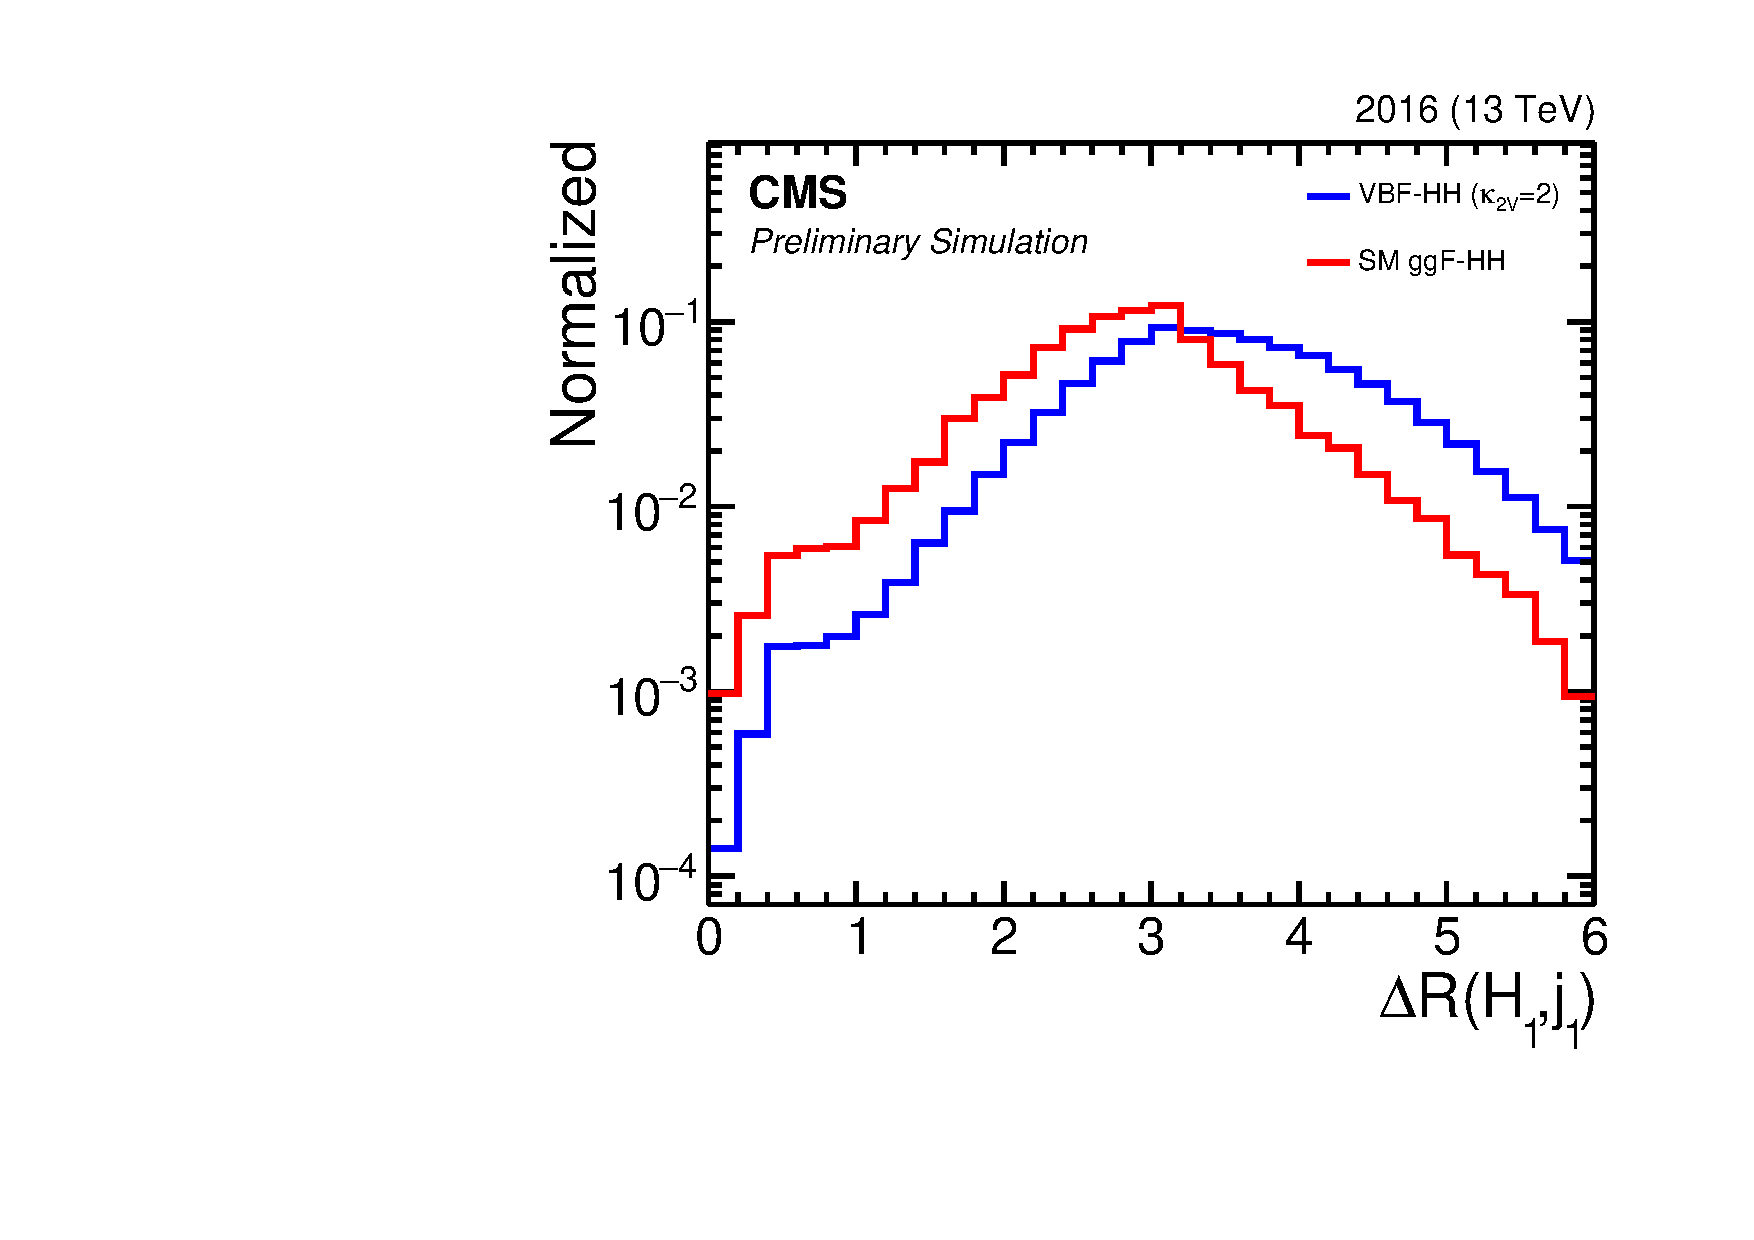
\includegraphics[width=0.27\linewidth]{Figures/AnalysisStrategy/eventselection/ggfkiller/2016ggfkiller/plot_2016_h_h1j1_deltaR.pdf}
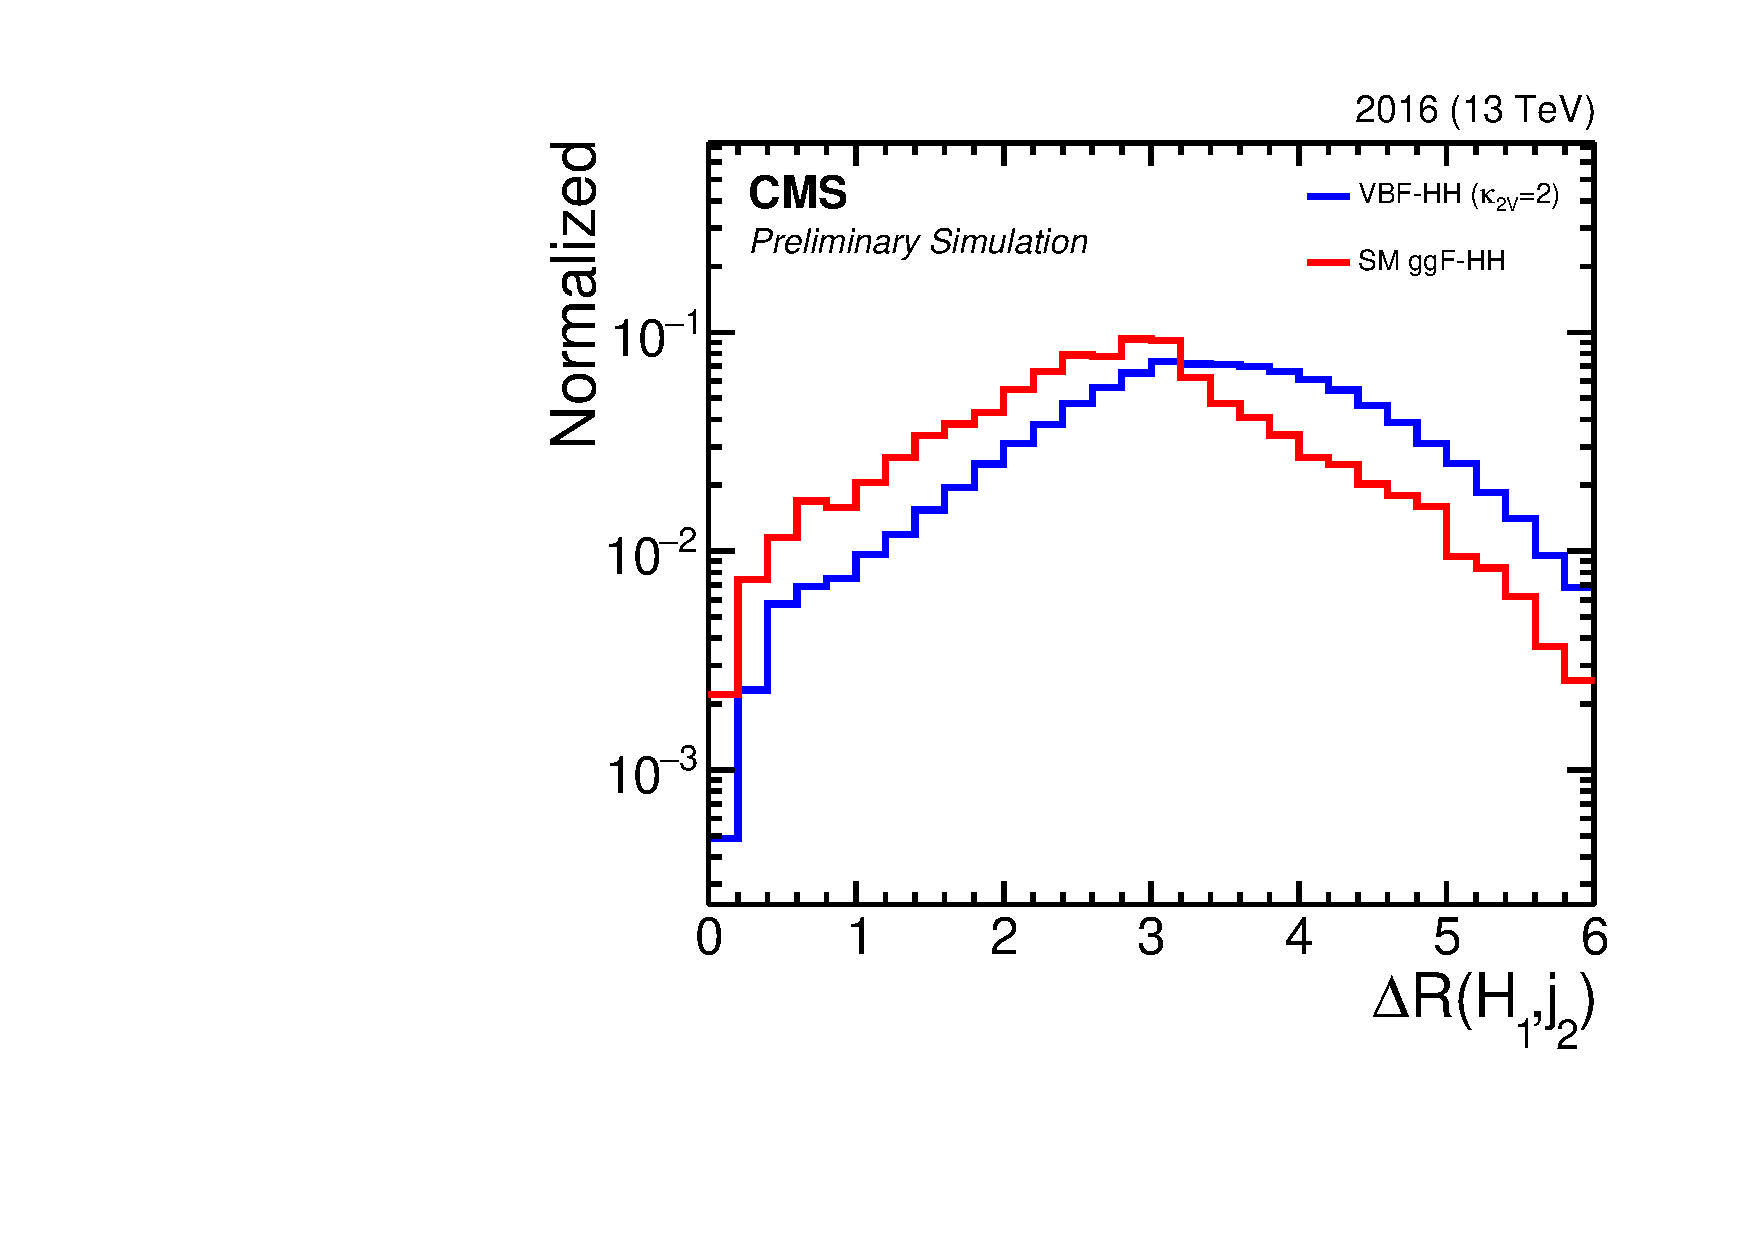
\includegraphics[width=0.27\linewidth]{Figures/AnalysisStrategy/eventselection/ggfkiller/2016ggfkiller/plot_2016_h_h1j2_deltaR.pdf}\\
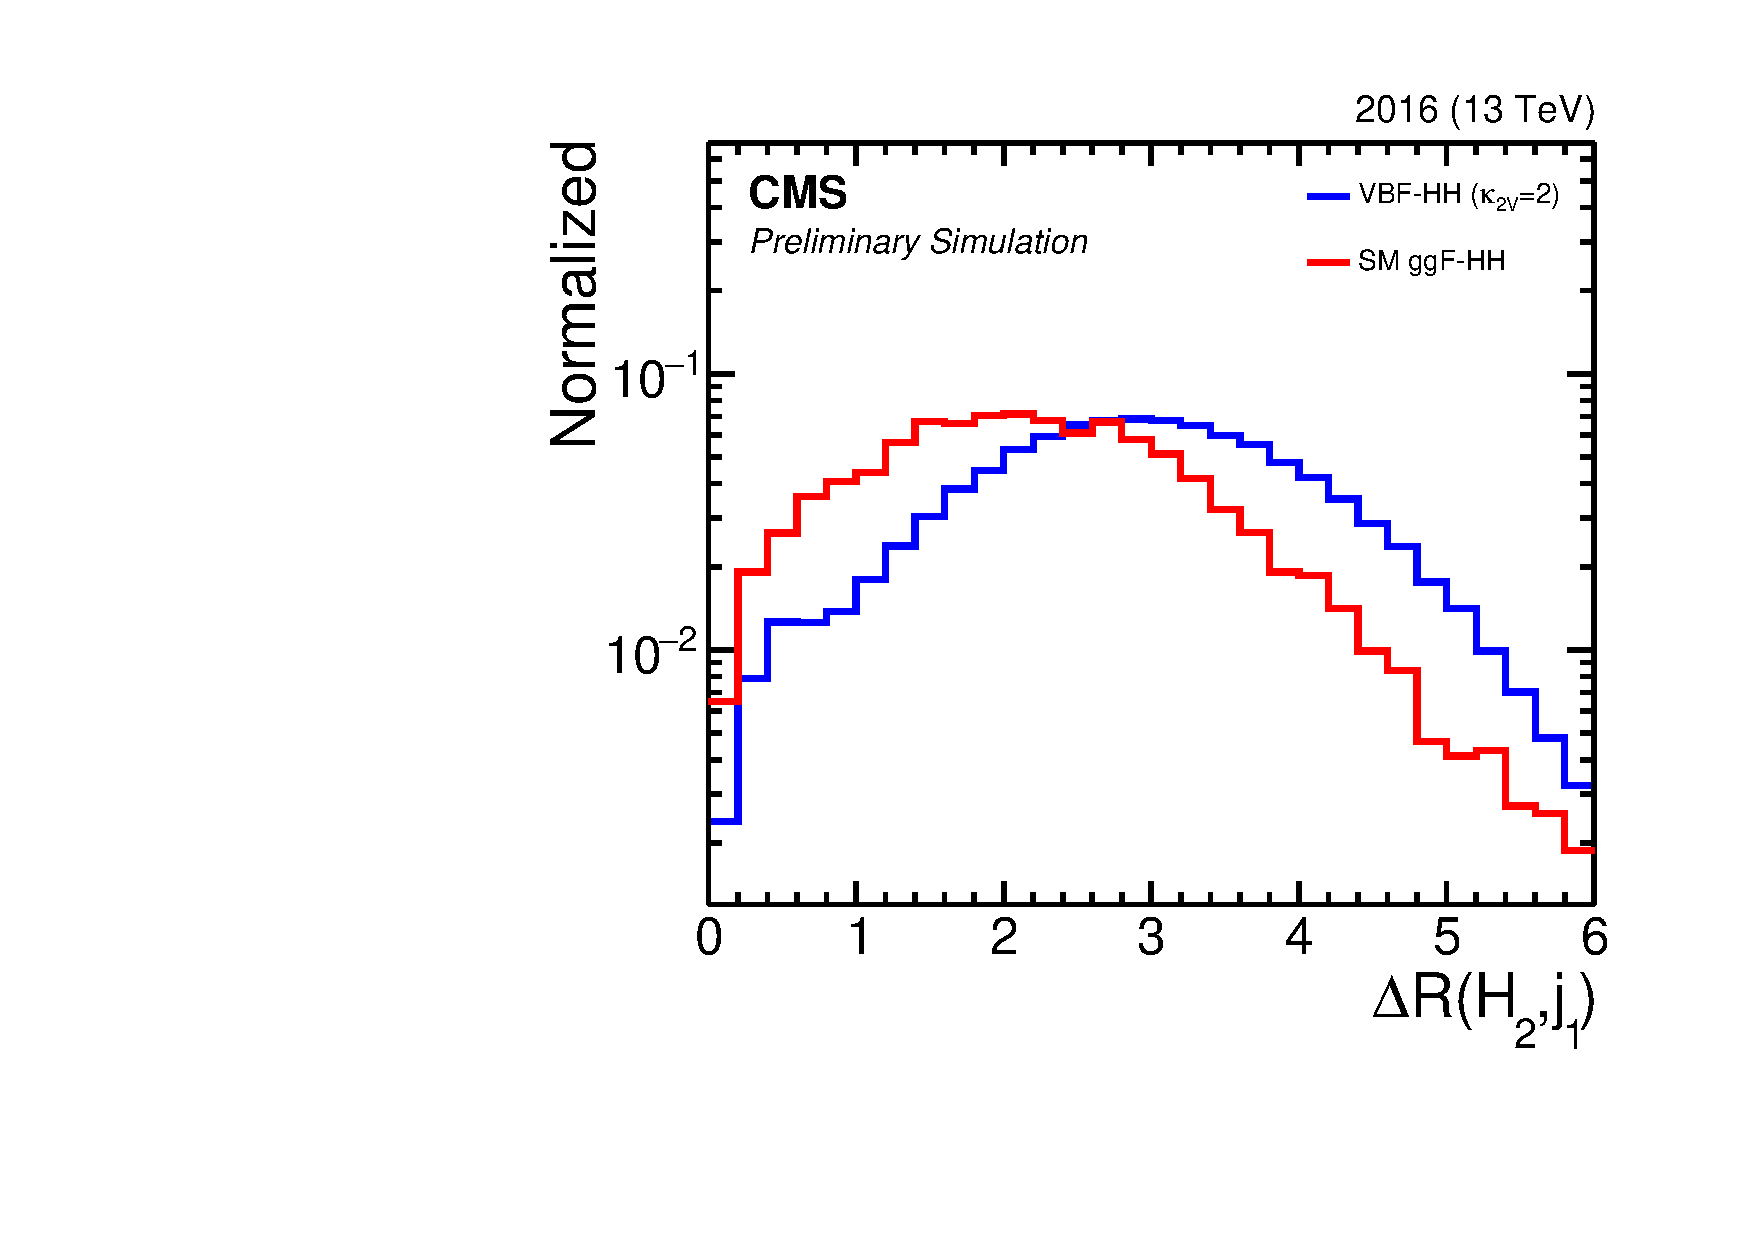
\includegraphics[width=0.27\linewidth]{Figures/AnalysisStrategy/eventselection/ggfkiller/2016ggfkiller/plot_2016_h_h2j1_deltaR.pdf}
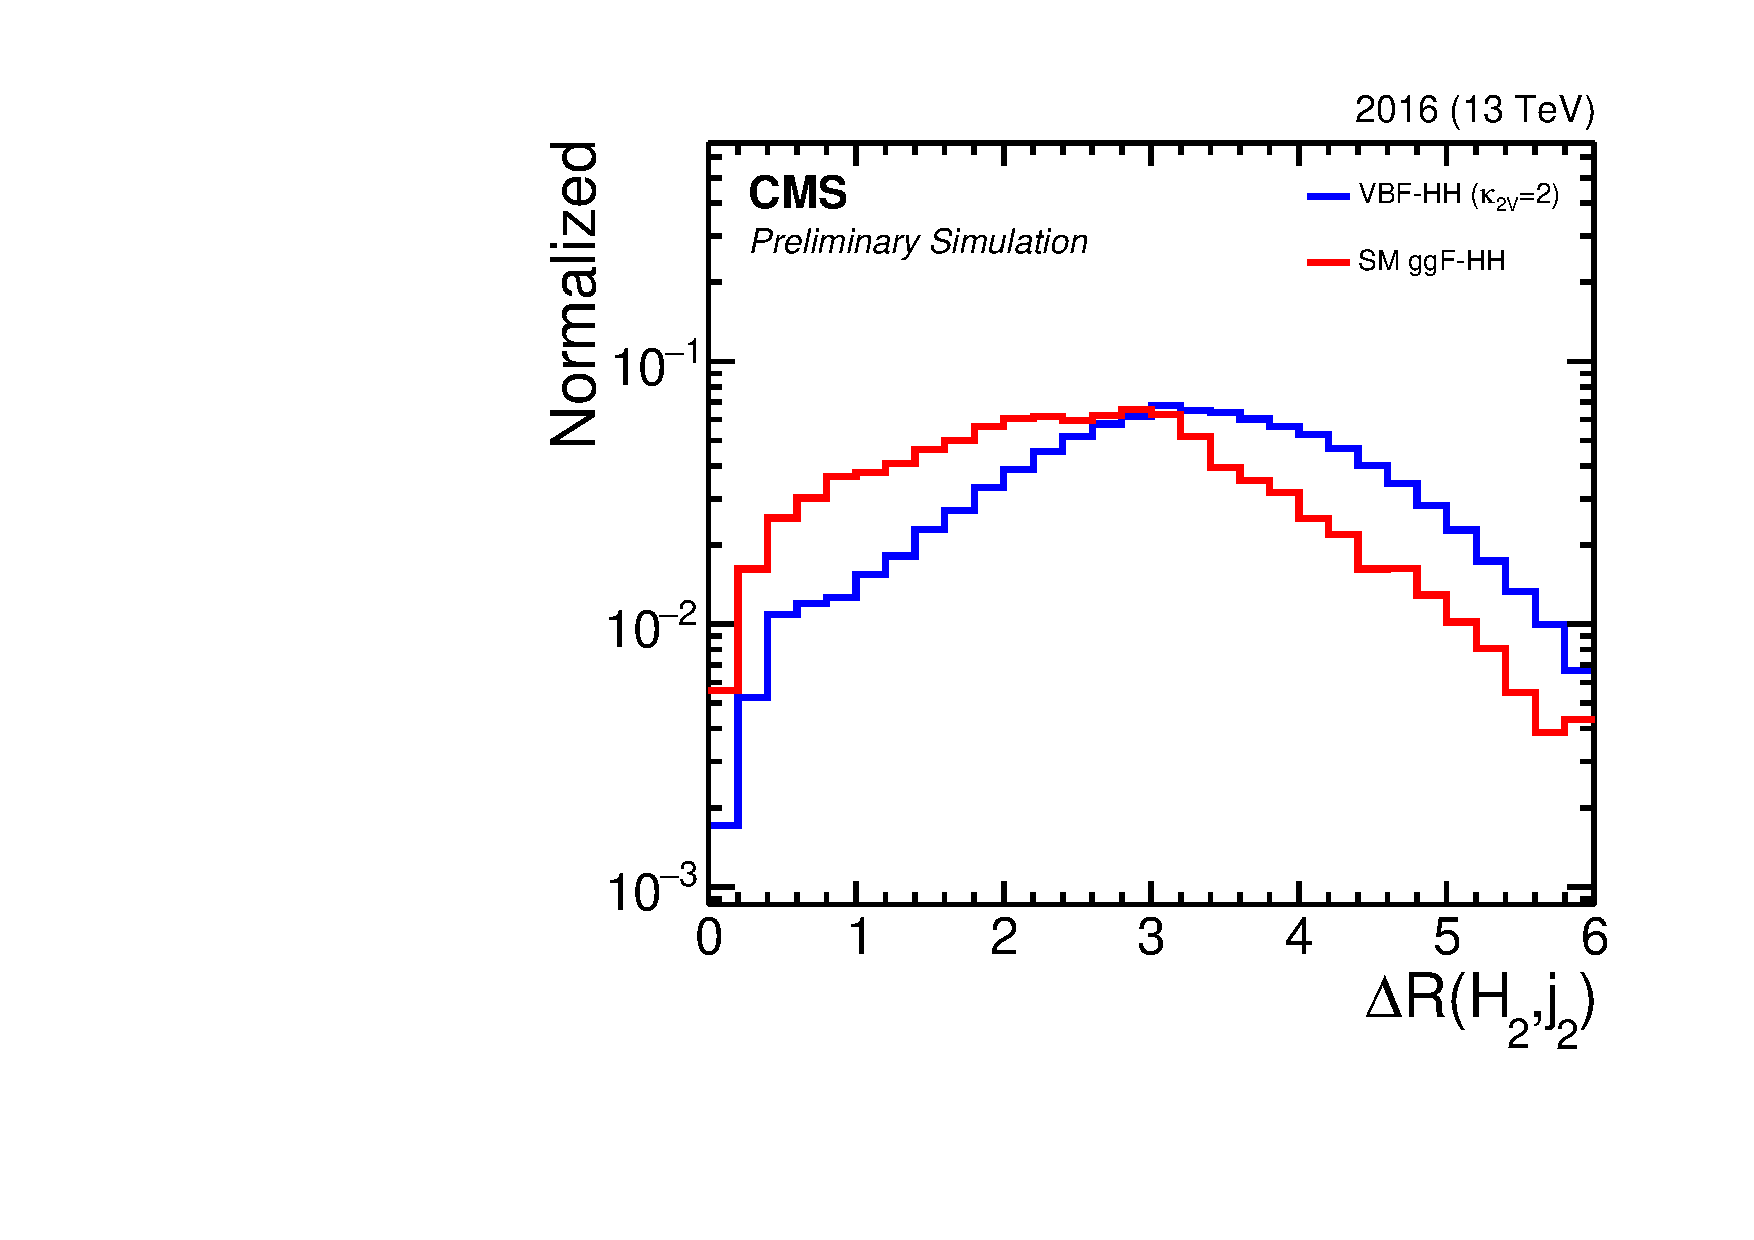
\includegraphics[width=0.27\linewidth]{Figures/AnalysisStrategy/eventselection/ggfkiller/2016ggfkiller/plot_2016_h_h2j2_deltaR.pdf}
\end{center}
\caption[Distribution of the ggFKiller input  variables in 2016 simulation]{Distribution of the ggFKiller input  variables in 2016 simulation. The VBF with $\kvv=2$ (signal) is in solid blue, whereas SM ggF (background) is in solid red.}
\label{event_selection:fig:bdtvariables2016}
\end{figure}

\clearpage

\begin{table}[htb]
\caption[Variables used to train the ggFKiller score]{\label{tab:ggfkillervars}Variables used to train the ggFKiller score. The product of Higgs centralities is defined as $\exp[-(\frac{\eta(H_{1})-\eta_{avg}}{\Delta\eta})^{2} - (\frac{\eta(H_{2})-\eta_{avg}}{\Delta\eta})^{2}]$, where \hbox{$\eta_{avg}=\frac{\eta(j_1)+\eta(j_2)}{2}$} and $\Delta\eta=\eta(j_1)-\eta(j_2)$.}
\centering
\begin{tabularx}{\textwidth}{l X}
	\hline
	Variable                                   & Meaning \\
	\hline
	$\mathrm{p_{T}(H_1)}$ ($\mathrm{p_{T}(H_2)}$)      & Transverse momentum of the $\hfst$ ($\hsnd$) candidate \\
	$\mathrm{p_{T}(j_1)}$ ($\mathrm{p_{T}(j_2)}$)      & Transverse momentum of the $\jfst$ ($\jsnd$) candidate \\
	$|\eta(\mathrm{jj})|$                      & VBF-jet pair pseudorapity   \\
	$\mathrm{M(jj)}$                           & VBF-jet pair invariant mass \\
	$\Delta\mathrm{R(H_1,H_2)}$	               & $\Delta\mathrm{R}$ distance between two Higgs bosons    \\
	$\Delta\mathrm{R(H_1,j_1)}$	               & $\Delta\mathrm{R}$ distance between $\hfst$ and $\jfst$ \\
	$\Delta\mathrm{R(H_1,j_2)}$	               & $\Delta\mathrm{R}$ distance between $\hfst$ and $\jsnd$ \\
	$\Delta\mathrm{R(H_2,j_1)}$	               & $\Delta\mathrm{R}$ distance between $\hsnd$ and $\jfst$ \\
	$\Delta\mathrm{R(H_2,j_2)}$	               & $\Delta\mathrm{R}$ distance between $\hsnd$ and $\jsnd$ \\
	$|\mathrm{\cos}(\theta)\mathrm{^{*}(j1)}|$ & $|\cos(\theta)|$ of $\jfst$ in the six-jet center of mass frame \\	
	$|\mathrm{\cos}(\theta)\mathrm{^{*}(j2)}|$ & $|\cos(\theta)|$ of $\jsnd$ in the six-jet center of mass frame \\ 	
    H1-centrality $\cdot$ H2-centrality        & Product of the Higgs boson centralities                         \\
	\hline
\end{tabularx}
\end{table}

The Figure~\ref{event_selection:fig:ggfkillershape} illustrates the distributions of the ggFKiller response of three signal simulated events in the pre-VBF event region: for VBF ($\kvv=2$), SM VBF and SM ggF. The observed response shows that VBF signal with anomalous $\kvv$ couplings have a high score, whereas the SM ggF signals a low score. It is important to note that the SM VBF signal tends to have a flat distribution and an enhancement at high ggFKiller values. 

\begin{figure}[htbp!]
\captionsetup[subfigure]{justification=centering}
\begin{center}
\subfloat[]{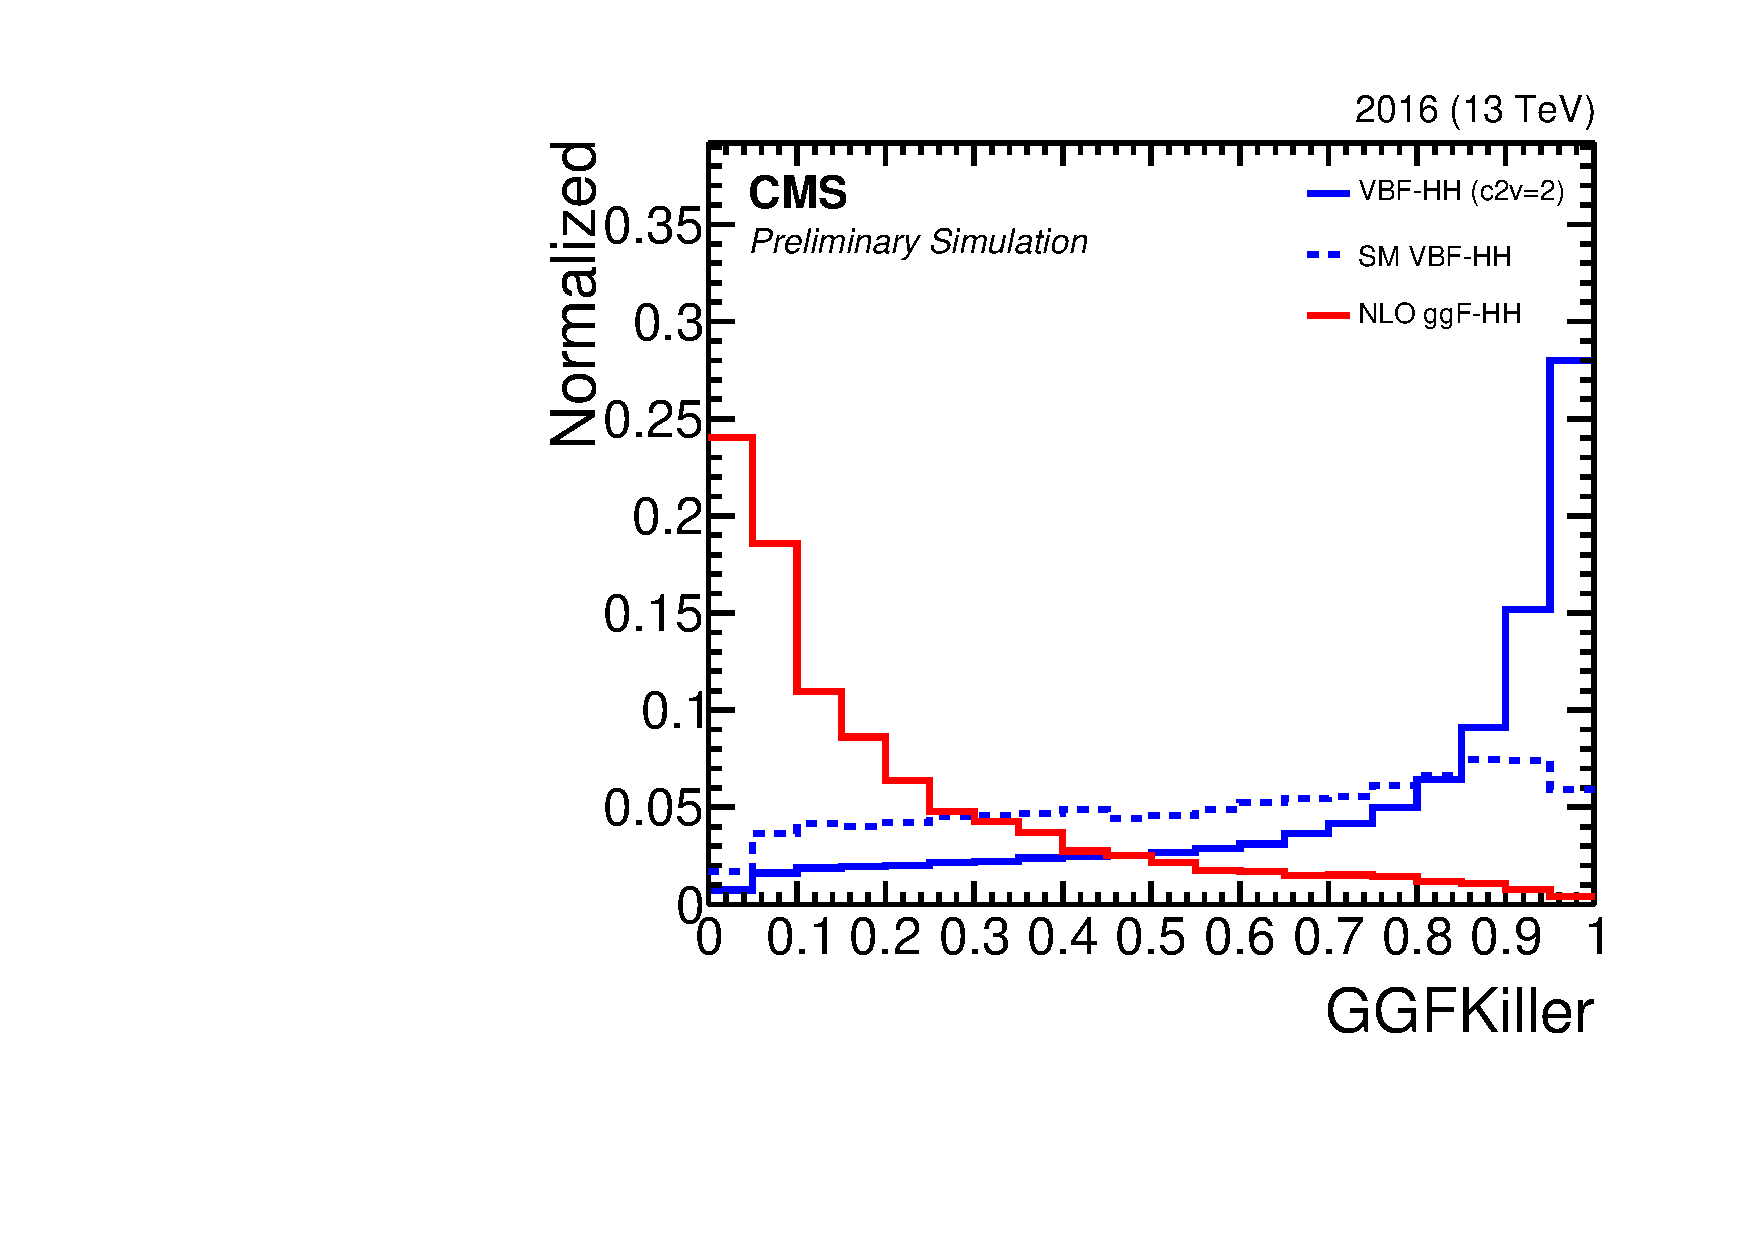
\includegraphics[width=0.325\linewidth]{Figures/AnalysisStrategy/eventselection/ggfkiller/shapes/plot_2016_h_GGFKiller.pdf}}
\subfloat[]{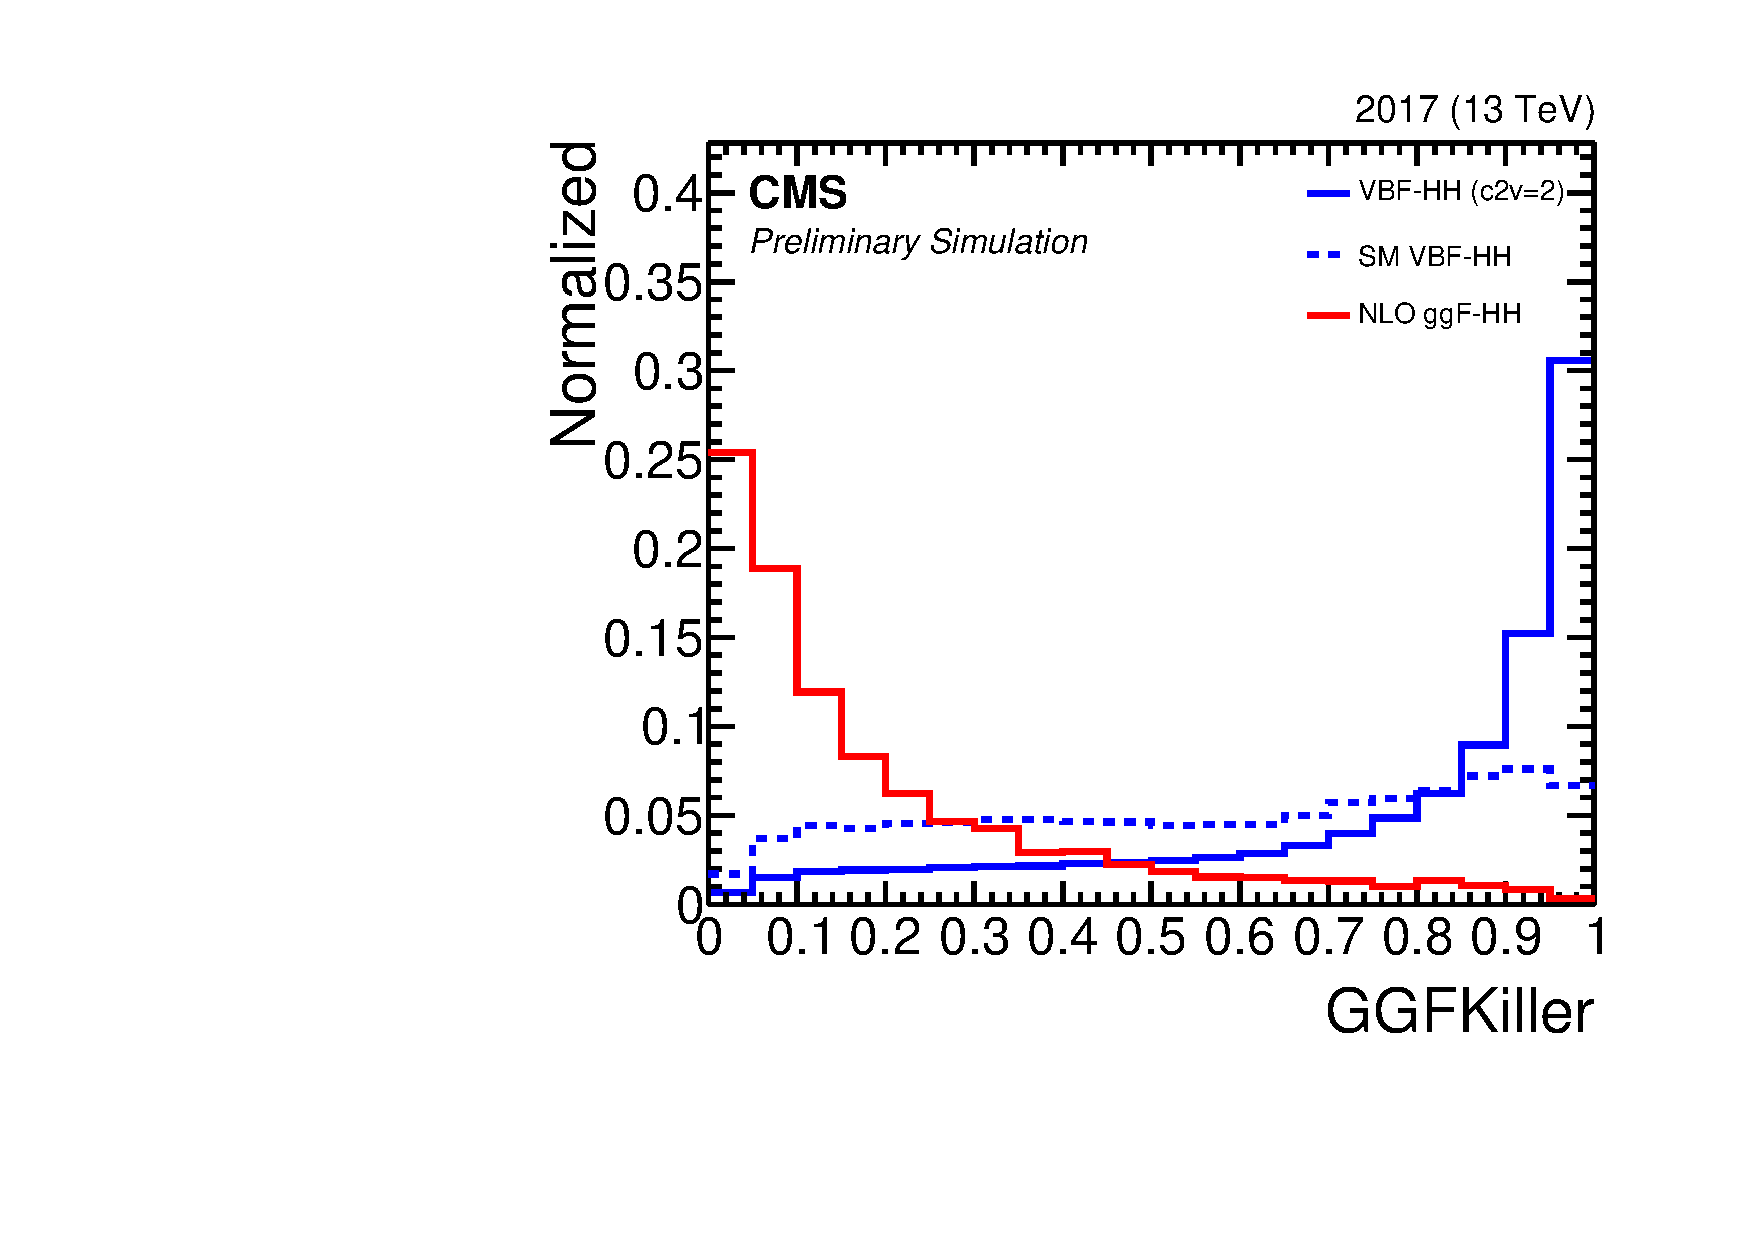
\includegraphics[width=0.325\linewidth]{Figures/AnalysisStrategy/eventselection/ggfkiller/shapes/plot_2017_h_GGFKiller.pdf}}
\subfloat[]{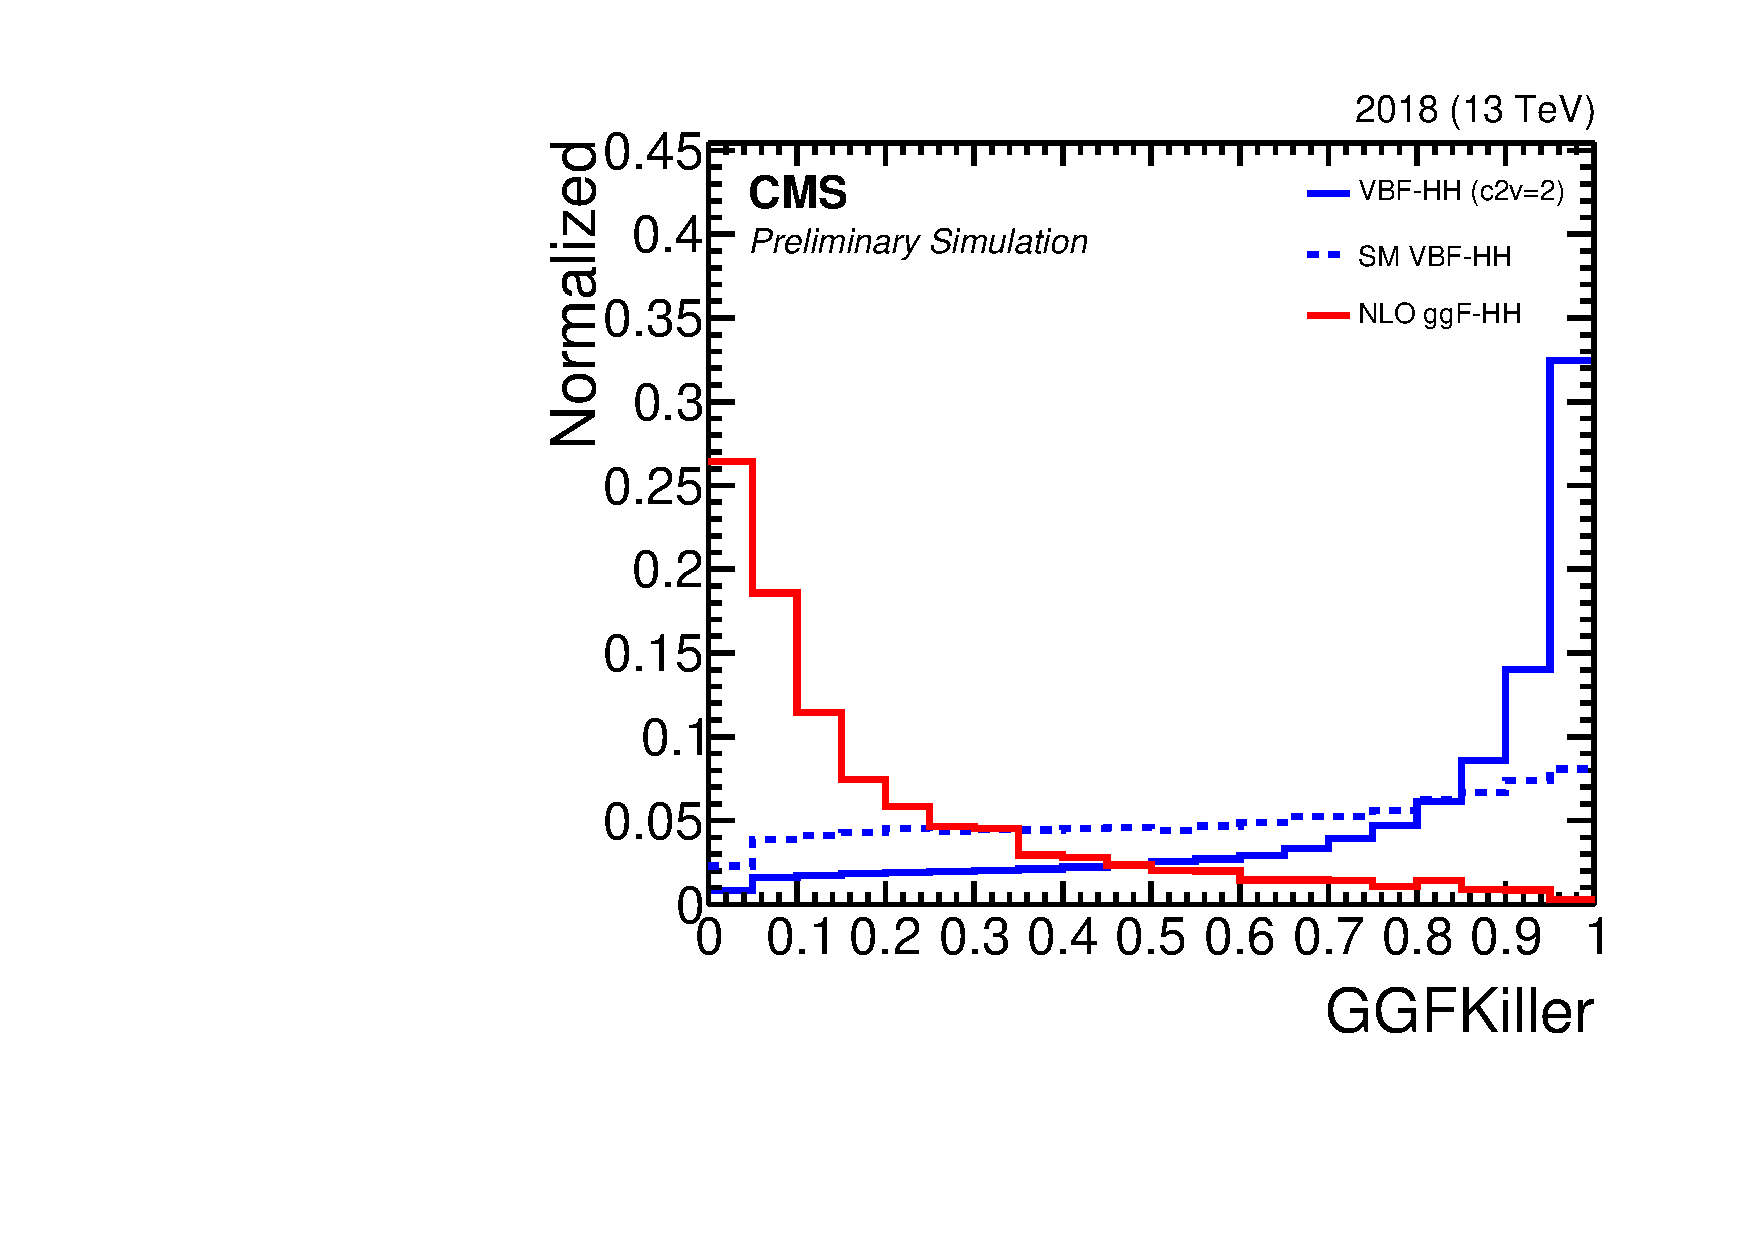
\includegraphics[width=0.325\linewidth]{Figures/AnalysisStrategy/eventselection/ggfkiller/shapes/plot_2018_h_GGFKiller.pdf}}
\end{center}
\caption[The ggFKiller output distributions]{The ggFKiller output distributions for VBF (c2v=2) (solid blue), SM VBF (dashed blue), SM ggF (solid red) signals in pre-VBF events. The simulated data-taking conditions correspond to A) 2016, B) 2017, C) 2018.}
\label{event_selection:fig:ggfkillershape}
\end{figure}

\subsection{Performance of the Production Mode Categorization}
The ggFKiller score is used to reduce the ggF signal leakage into pre-VBF events and to create a more pure production mode categories. For this search, a score of ggFKiller=0.5 is found to be the optimal to further categorize events by production mode. The choice of this boundary is discussed in Subsection~\ref{subsec:optimization}. The ggF Category combines two groups: Pre-ggF events, and Pre-VBF events with ggFKiller between 0 and 0.5, whereas the VBF Category is composed of Pre-VBF events with ggFKiller between 0.5 and 1. 
 
Event yields of the ggF and VBF categories are reported in Table~\ref{event_selection:tab:categorization}. Depending on the year, we observe that the ggF category contains around 96-97.0\% of the SM ggF signal. Furthermore, the categorization has improved the relative ratios between SM ggF with respect to the VBF signals in the table: (1) SM ggF / SM VBF is around 4.5-5.3, and (2) SM ggF / VBF ($\kvv=2$) is 0.03-0.07.

\begin{table}[htb]
\caption[Event yields of data and MC simulation after categorization into ggF and VBF categories]{\label{event_selection:tab:categorization}Event yields of data and MC simulation after categorization into ggF and VBF categories. The processes ggF, VBF and VBF$(\kvv=2)$ are multiplied by a factor of $10^{2}$.}
\centering
\begin{tabularx}{\textwidth}{l r r r r r r}
   	\hline
	Dataset/Categ.            & 2016/ggF       &   2016/VBF     &    2017/ggF    & 2017/VBF       & 2018/ggF       &  2018/VBF     \\
	\hline
	ggF             &    1559.4 &      58.0 &    1003.3 &      31.2 &    1798.0 &      67.9 \\
	VBF              &      16.5 &      10.8 &      11.9 &       6.9 &      22.2 &      14.7 \\
	VBF($\kvv=2$)   &     805.1 &     778.9 &     558.5 &     466.6 &    1152.6 &    1058.8 \\
	QCD                       &  165189.0 &    8776.9 &   74259.5 &    2906.6 &  120202.3 &    5920.5 \\
	$\ttbar$                  &   10458.8 &     916.1 &    6121.9 &     462.7 &   12928.2 &    1089.8 \\
	Single Higgs              &     684.4 &      53.6 &     483.5 &      26.7 &     936.7 &      57.1 \\
	ZZ$\rightarrow$4b         &      36.7 &       0.9 &      21.4 &       0.6 &      37.6 &       1.0 \\
	Total MC Bkg.             &  176368.9 &    9747.5 &   80886.3 &    3396.6 &  134104.8 &    7068.4 \\
	Data                      &  211586 &   11286 &  159965 &    8129 &  245374 &   15207 \\
	\hline
\end{tabularx}
\end{table}

The production mode classification has a very good performance. For ggF signals, we observe that the fraction of events classified in the ggF categories as a function of the $\kl$ coupling is at least $\sim95\%$ and has a more or less flat $\kl$-dependency, as presented in Figure~\ref{event_selection:fig:fractionggfvbfcategs_vs_kl}~A).  Due to the training conditions, the VBF signal efficiency after the ggFKiller cut is the most optimal for $\kvv$ anomalous couplings. For VBF signals, we observe a good efficiency of signal events passing the ggFKiller cut as a function of the $\kvv$ and $\kv$ couplings, as illustrated Figure~\ref{event_selection:fig:fractionggfvbfcategs_vs_kl}~(B-D).

\begin{figure}[htbp!]
\captionsetup[subfigure]{justification=centering}
\begin{center}
\subfloat[]{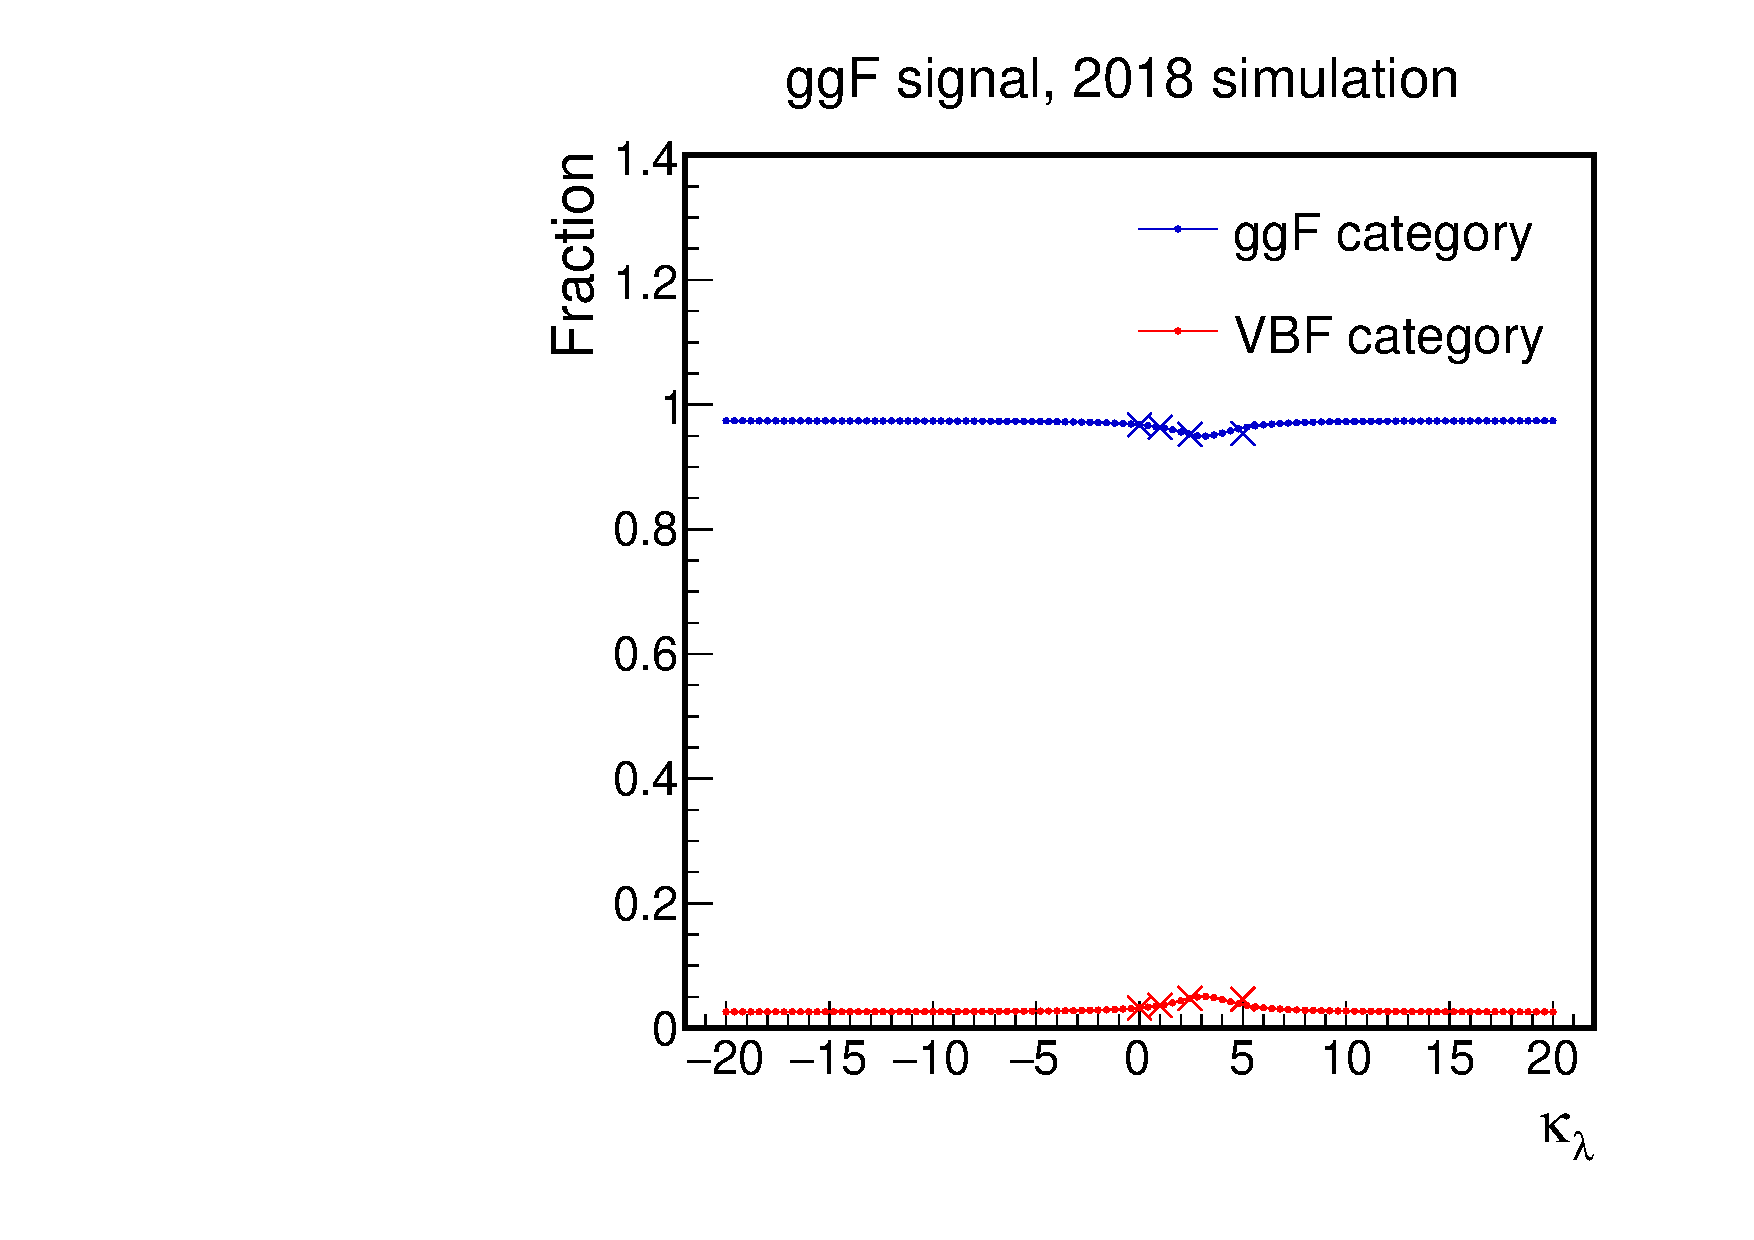
\includegraphics[width=0.45\linewidth]{Figures/AnalysisStrategy/eventselection/efficiencies/frac_categ_2018_GGFvsVBF_vs_kl.pdf}} 
\subfloat[]{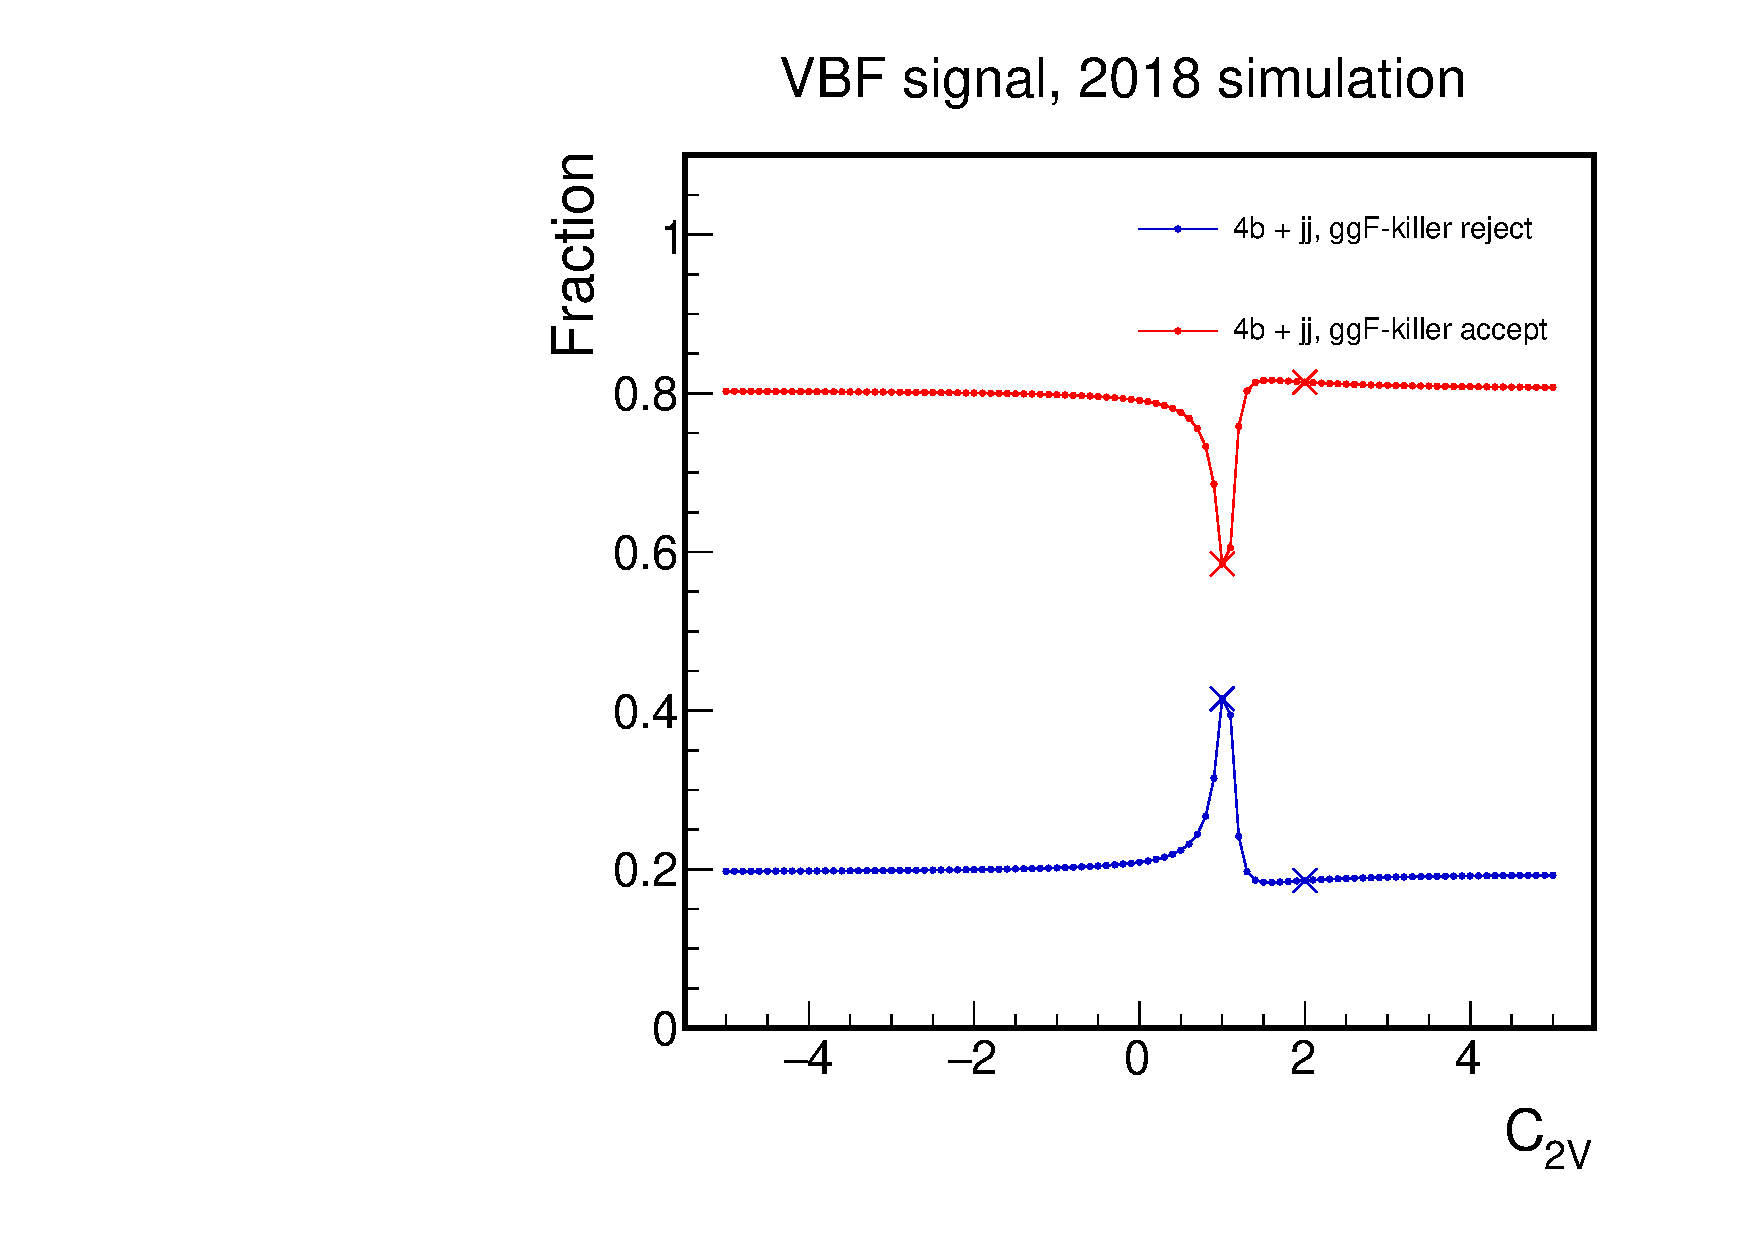
\includegraphics[width=0.45\linewidth]{Figures/AnalysisStrategy/eventselection/efficiencies/frac_categ_2018_GGFvsVBF_ForVBFEvts_VFBsignal_vs_C2V.pdf}} \\
\subfloat[]{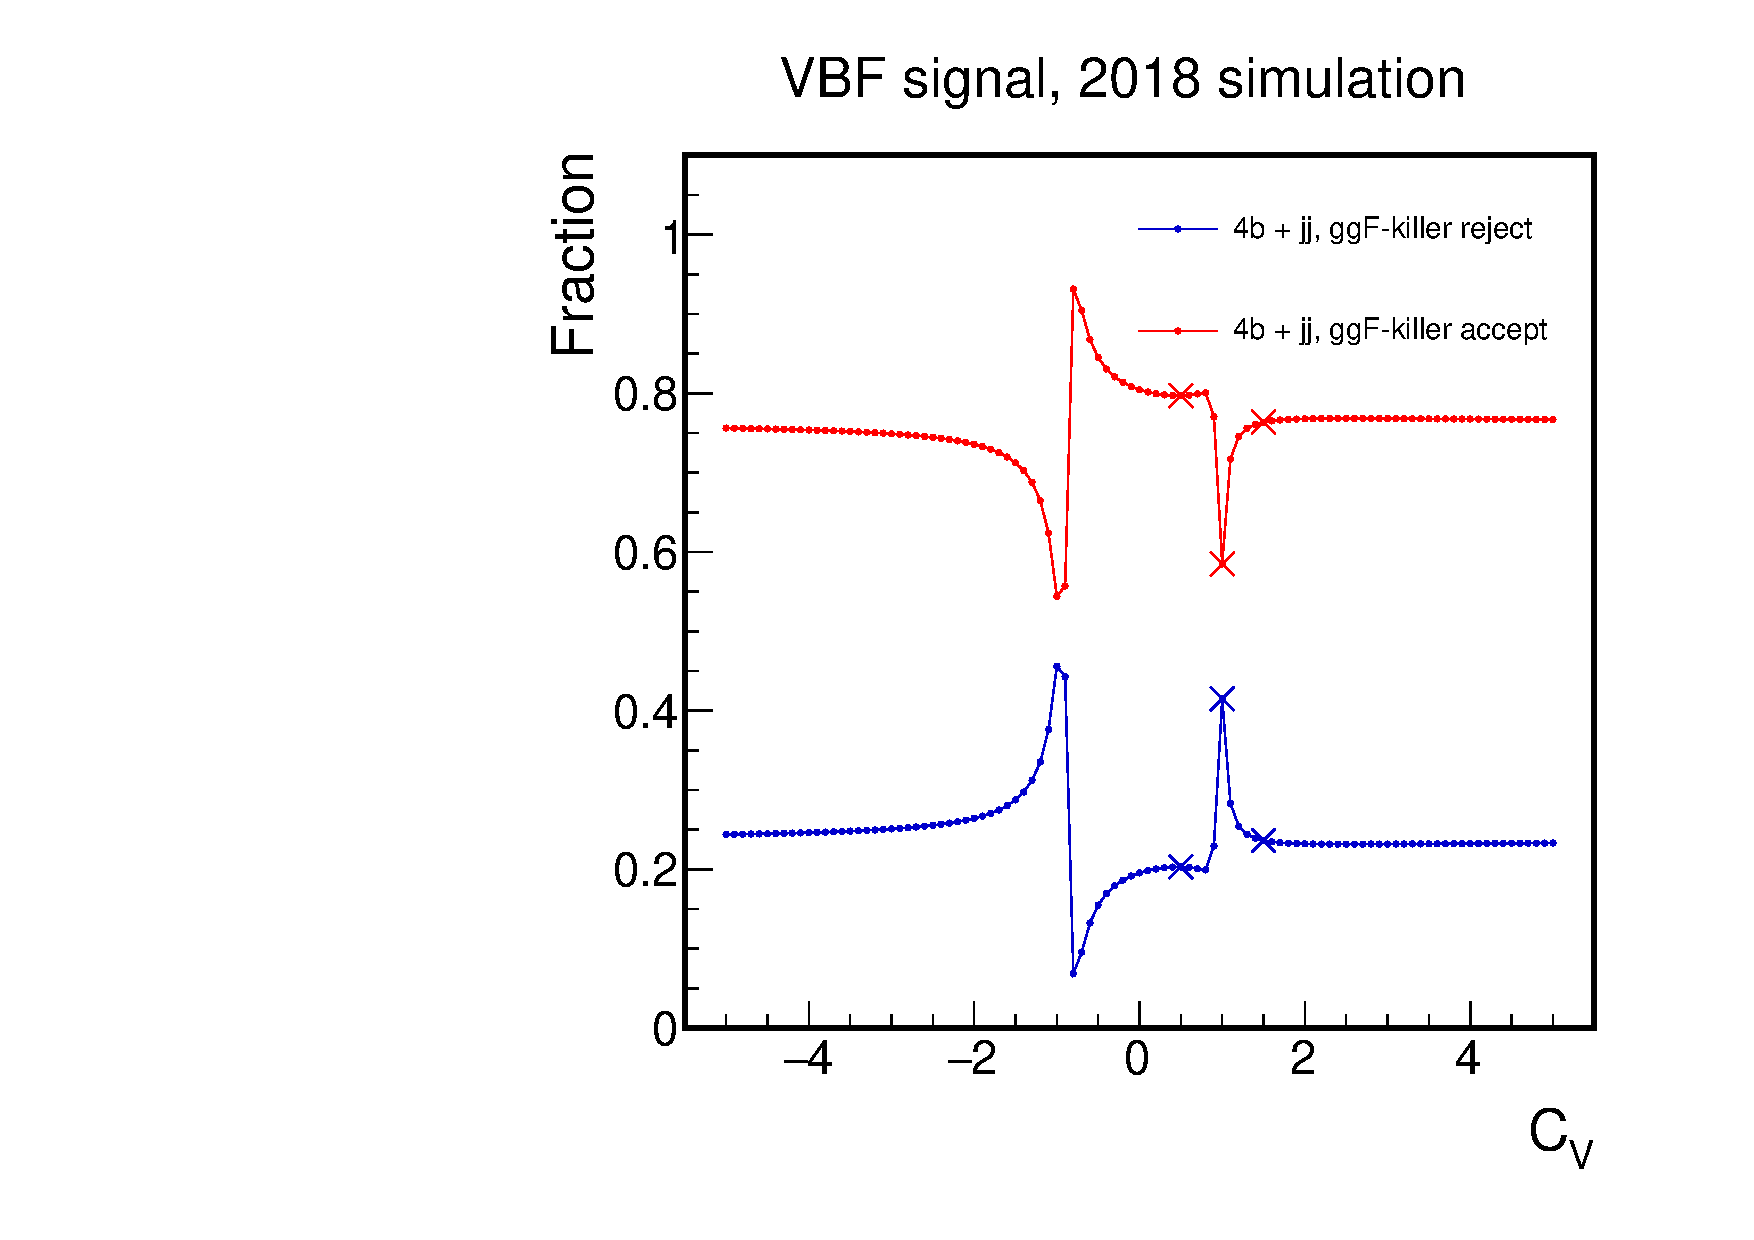
\includegraphics[width=0.45\linewidth]{Figures/AnalysisStrategy/eventselection/efficiencies/frac_categ_2018_GGFvsVBF_ForVBFEvts_VFBsignal_vs_CV.pdf}} 
\subfloat[]{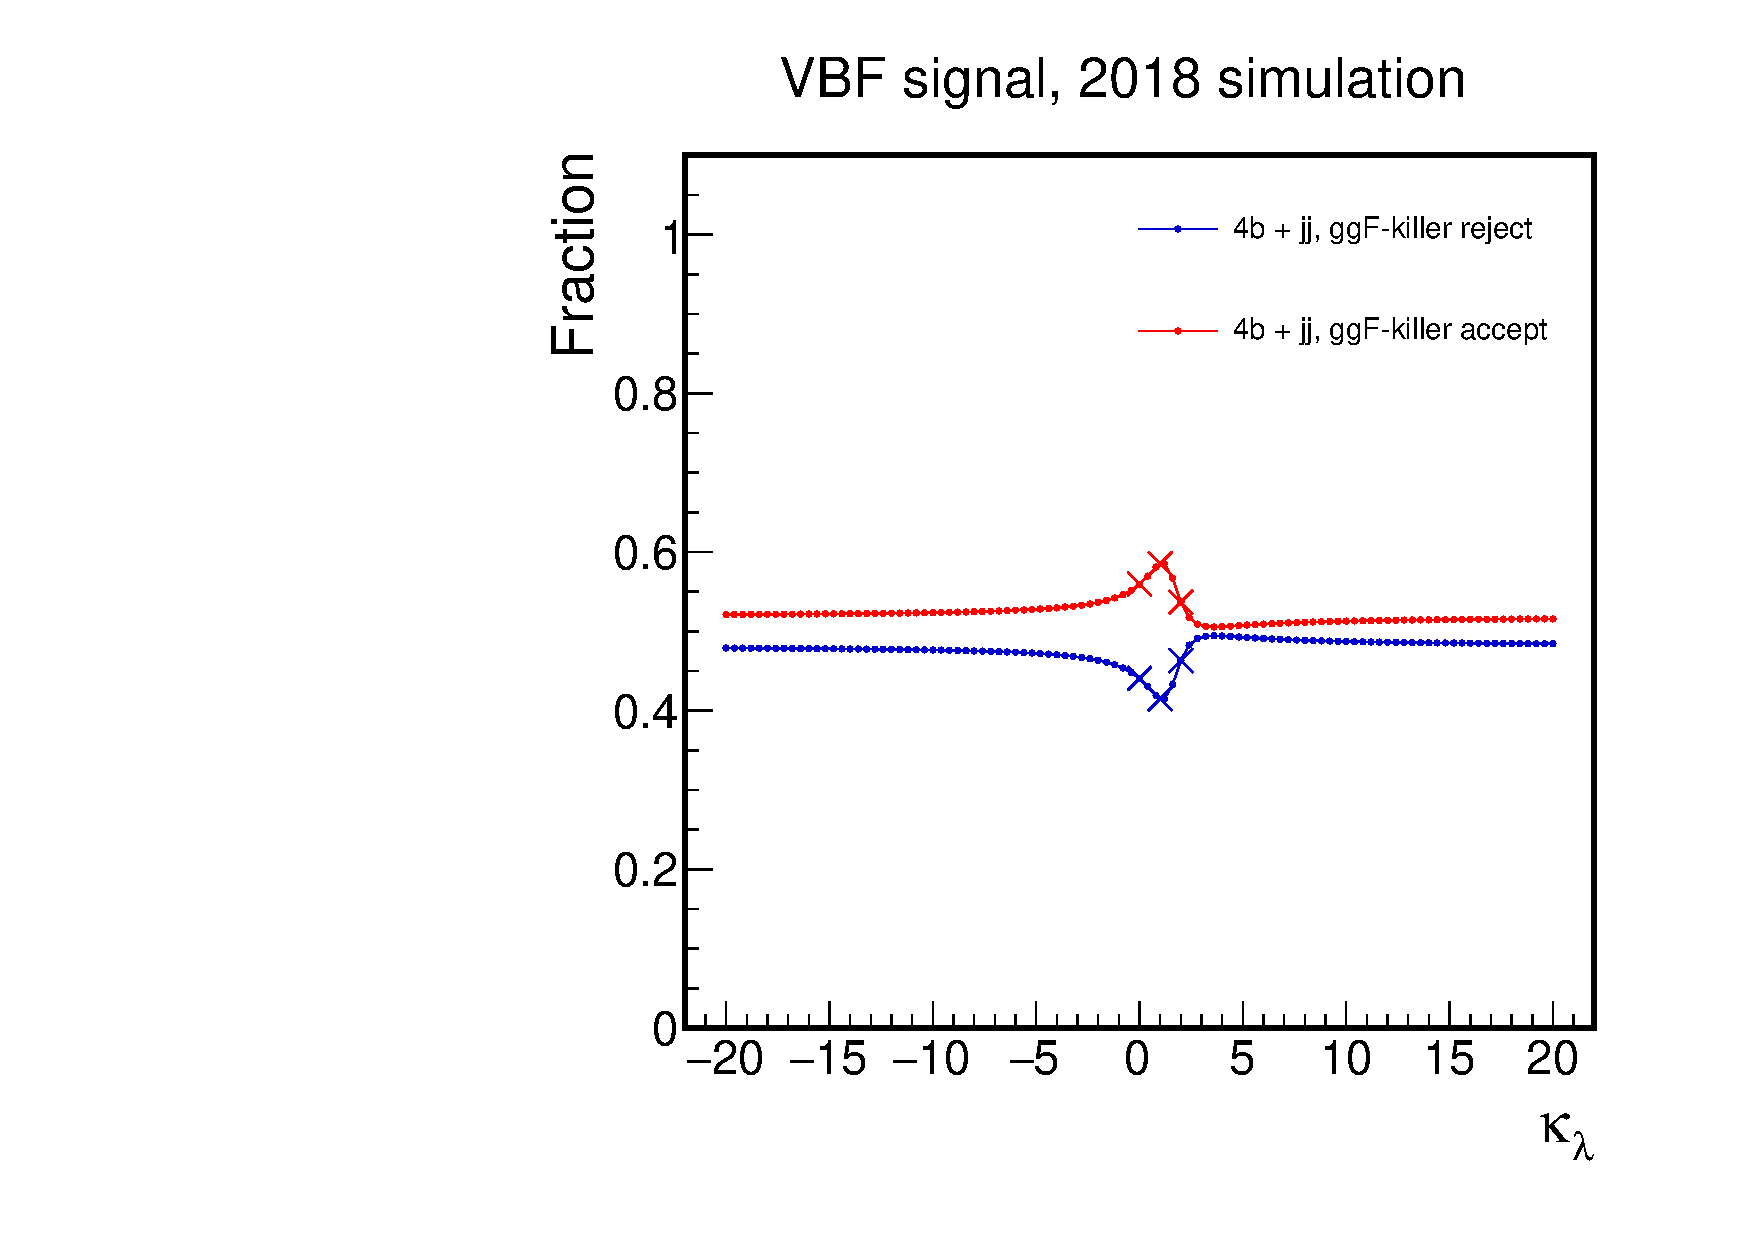
\includegraphics[width=0.45\linewidth]{Figures/AnalysisStrategy/eventselection/efficiencies/frac_categ_2018_GGFvsVBF_ForVBFEvts_VFBsignal_vs_kl.pdf}} \\
\end{center}
\caption[Performance of the ggFKiller in the production mode classification as a function of the couplings]{Performance of the ggFKiller in the production mode classification as a function of the couplings.  A) Fraction of inclusive ggF signal events that are classified in the ggF and VBF cat-
egories as a function of $\kl$. B/C/D) Fraction of VBF signal events from the pre-VBF region classified in the ggF category and VBF categories as function of the $\kvv/\kv/\kl$ coupling. The crosses indicate the values obtained directly from the simulated samples, serving as cross-check to the values computed with the signal modeling procedure represented by the full
circles. The simulated data-taking conditions correspond to 2018.}

\label{event_selection:fig:fractionggfvbfcategs_vs_kl}
\end{figure}

\clearpage

\section{Event Regions} \label{sec:regions}
The analysis strategy demands the definition of regions of the phase space, which events are used  to perform dedicated tasks such as background modeling and signal strength measurement. In this work, the set of preselected events are defined depending on the b-tagging multiplicity and the invariant masses of the two reconstructed Higgs boson candidates ($\hfstm$ and $\hsndm$). The definition and purpose of these regions are explained in this section.

\subsection{The `4b' and `3b' Regions} \label{sec:btagregions}

All events passing the trigger and preselection requirements presented in Section~\ref{sec:preselection} are denominated as `4b' events. On the other hand, events passing the trigger in which the fourth jet by b-tagging score fails the preselection b-tagging cut (Table~\ref{eventselection:tab:bjetreq}) are denominated as the `3b' events. Event yields for data and MC simulation are presented in Table~\ref{event_selection:tab:presel} for the `3b' region. 

\begin{table}[htb]
\caption[Event yields of data and MC simulation after categorization requirements in the 3b region]{\label{event_selection:tab:3bdatamc}Event yields of data and MC simulation after categorization requirements in the 3b region. The processes ggF, VBF and VBF$(\kvv=2)$ are multiplied by a factor of $10^{2}$.}
\centering
\begin{tabularx}{\textwidth}{l r r r r r r}
	\hline
	Dataset/Categ.          & 2016/ggF  & 2016/VBF  & 2017/ggF  & 2017/VBF  & 2018/ggF   & 2018/VBF \\
	\hline
	ggF            &    2419.2 &      77.8 &    1188.9 &      32.0 &     2404.3 &      78.7 \\ 
	VBF            &      48.9 &      16.2 &      29.3 &       7.2 &       62.0 &      18.9 \\ 
	VBF$(\kvv=2)$  &    1424.8 &     880.0 &     719.7 &     343.0 &     1689.9 &     886.7 \\
	QCD                     & 1725011.0 &   68994.7 &  532655.1 &   16344.5 &  1058750.0 &   43059.3 \\ 
	$\mathrm{t\overline{t}}$&  100496.2 &    5819.9 &   50288.3 &    2489.5 &   111774.6 &    6518.1 \\ 
	Single Higgs            &    1657.5 &     106.9 &     973.8 &      45.8 &     2053.0 &     107.3 \\ 
	ZZ$\rightarrow$4b       &      90.9 &       2.0 &      41.6 &       1.0 &       85.3 &       2.1 \\
	Total MC Bkg.           & 1827255.6 &   74923.5 &  583958.8 &   18880.8 &  1172662.9 &   49686.8 \\
	Data                    &   2285706 &   86800 & 1263243&   49416 &  2273811 &  107918 \\
	\hline
\end{tabularx}
\end{table}

Depending on the production mode category, there are 7-10 times more data events in the 3b region than in the 4b region. While this signal contamination in the 3b region cannot be avoided and is due to the limited efficiency of the b tag algorithm, the signal to background ratio in the 3b region is significantly small compared to the 4b region. For instance, for 2016 SM ggF signal, the corresponding signal/background at the ggF 3b region is about 15\% the one in the ggF 4b region. Therefore, the `3b' region data events are suitable as input for a data-driven background model and further explained in Chapter~\ref{chapter:modeling}.

\clearpage

\subsection{Analysis and Validation Regions} \label{sec:analysisregions}
The ultimate goal of the dissertation is to extract a possible signal from the collected data. A key step is then to define a signal-enriched region with large signal-to-background ratio for the main data analysis, denominated analysis signal region ($\mathrm{A_{SR}}$). At the same time, we have to define a region with low signal-to-background ratio and close to the SR to construct the background model, named analysis control region ($\mathrm{A_{CR}}$). 

In the two-dimensional phase space of the two reconstructed Higgs boson masses or $\hfstm$-$\hsndm$ plane, the HH signal events populate the region surrounding the peak located around $\hfstm$=125 GeV and $\hsndm$=120 GeV. Note that the difference between $\hfstm$ and $\hsndm$ arises from the $\pt$ ordering imposed to the Higgs boson candidates. For this search, the optimal choice of the $\mathrm{A_{SR}}$ and $\mathrm{A_{CR}}$ regions is a circle (eq. \ref{eq:sr}) and a ring (eq. \ref{eq:cr}) centered at the coordinates (C1,C2)=(125 GeV,120 GeV) in the $\hfstm$-$\hsndm$ plane. The $\mathrm{A_{SR}}$ and $\mathrm{A_{CR}}$ regions are sketched in the Figure~\ref{event_selection:fig:vsrcr}.
\begin{equation}\label{eq:sr}
\sqrt{ \left(\hfstm-C_1\right)^{2} +   \left(\hsndm-C_2\right)^{2}   } < 25~\mathrm{GeV} 
\end{equation}
\begin{equation}\label{eq:cr}
25~\mathrm{GeV} \leq \sqrt{ \left(\hfstm-C_1\right)^{2} + \left(\hsndm-C_2\right)^{2}   } < 50~\mathrm{GeV}\end{equation}
\begin{figure}[ht!]
\centering
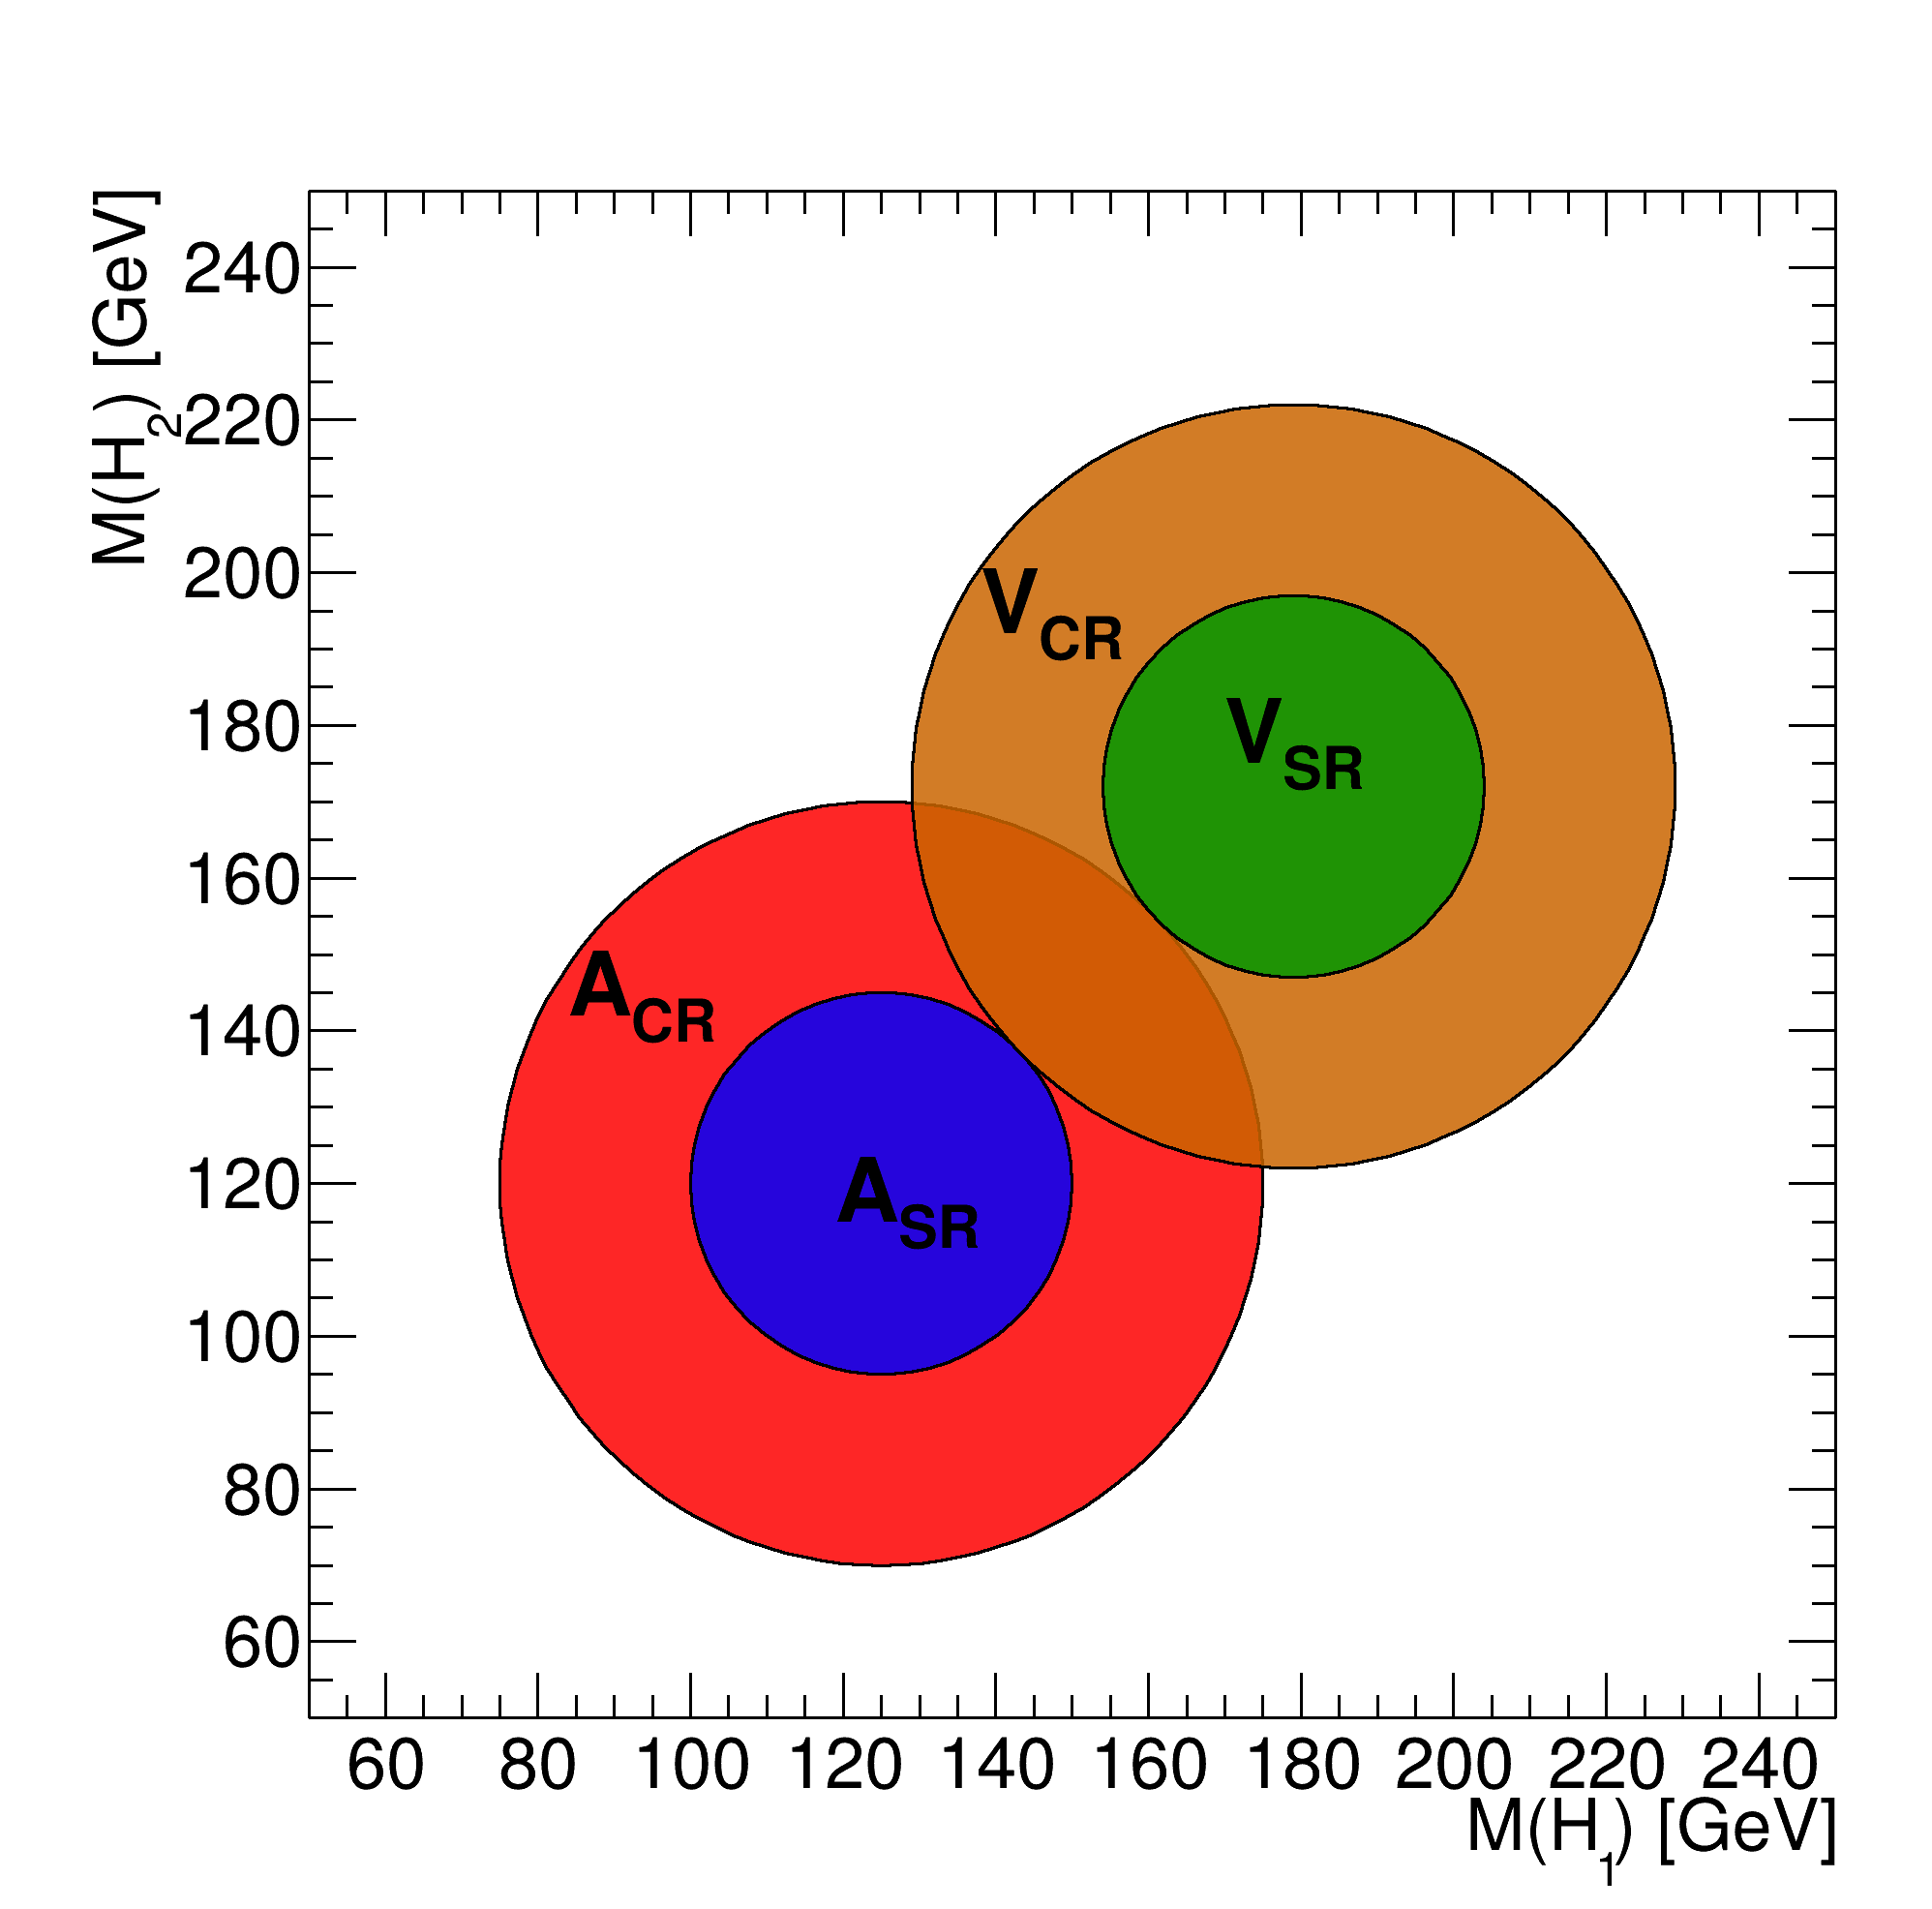
\includegraphics[width=0.4\linewidth]{Figures/AnalysisStrategy/eventselection/regions/vsrcrcircle.png}
\caption[Definition of signal and control regions for the analysis and validation regions]{Definition of signal and control regions for the analysis and validation regions.}
\label{event_selection:fig:vsrcr}
\end{figure}

As will be detailed in Chapter~\ref{chapter:modeling}, events from a phase space orthogonal to $\mathrm{A_{SR}}$ is needed to fully validate the background model. To that end, we define the validation signal region circle ($\mathrm{V_{SR}}$) and validation control regions ring ($\mathrm{V_{CR}}$) also in the $\hfstm$-$\hsndm$ plane but shifting their center along the pairing diagonal line to (C1,C2)=(179 GeV,172 GeV). The analysis and validation regions used in this dissertation are illustrated in the sketch in Figure~\ref{event_selection:fig:vsrcr}. Furthermore, the distribution of the SM ggF and VBF ($\kvv=2$) signal simulated events across the regions are shown in Figure~\ref{event_selection:fig:vsrcrsignal}.
\begin{figure}[htbp!]
\captionsetup[subfigure]{justification=centering}
\centering
\subfloat[]{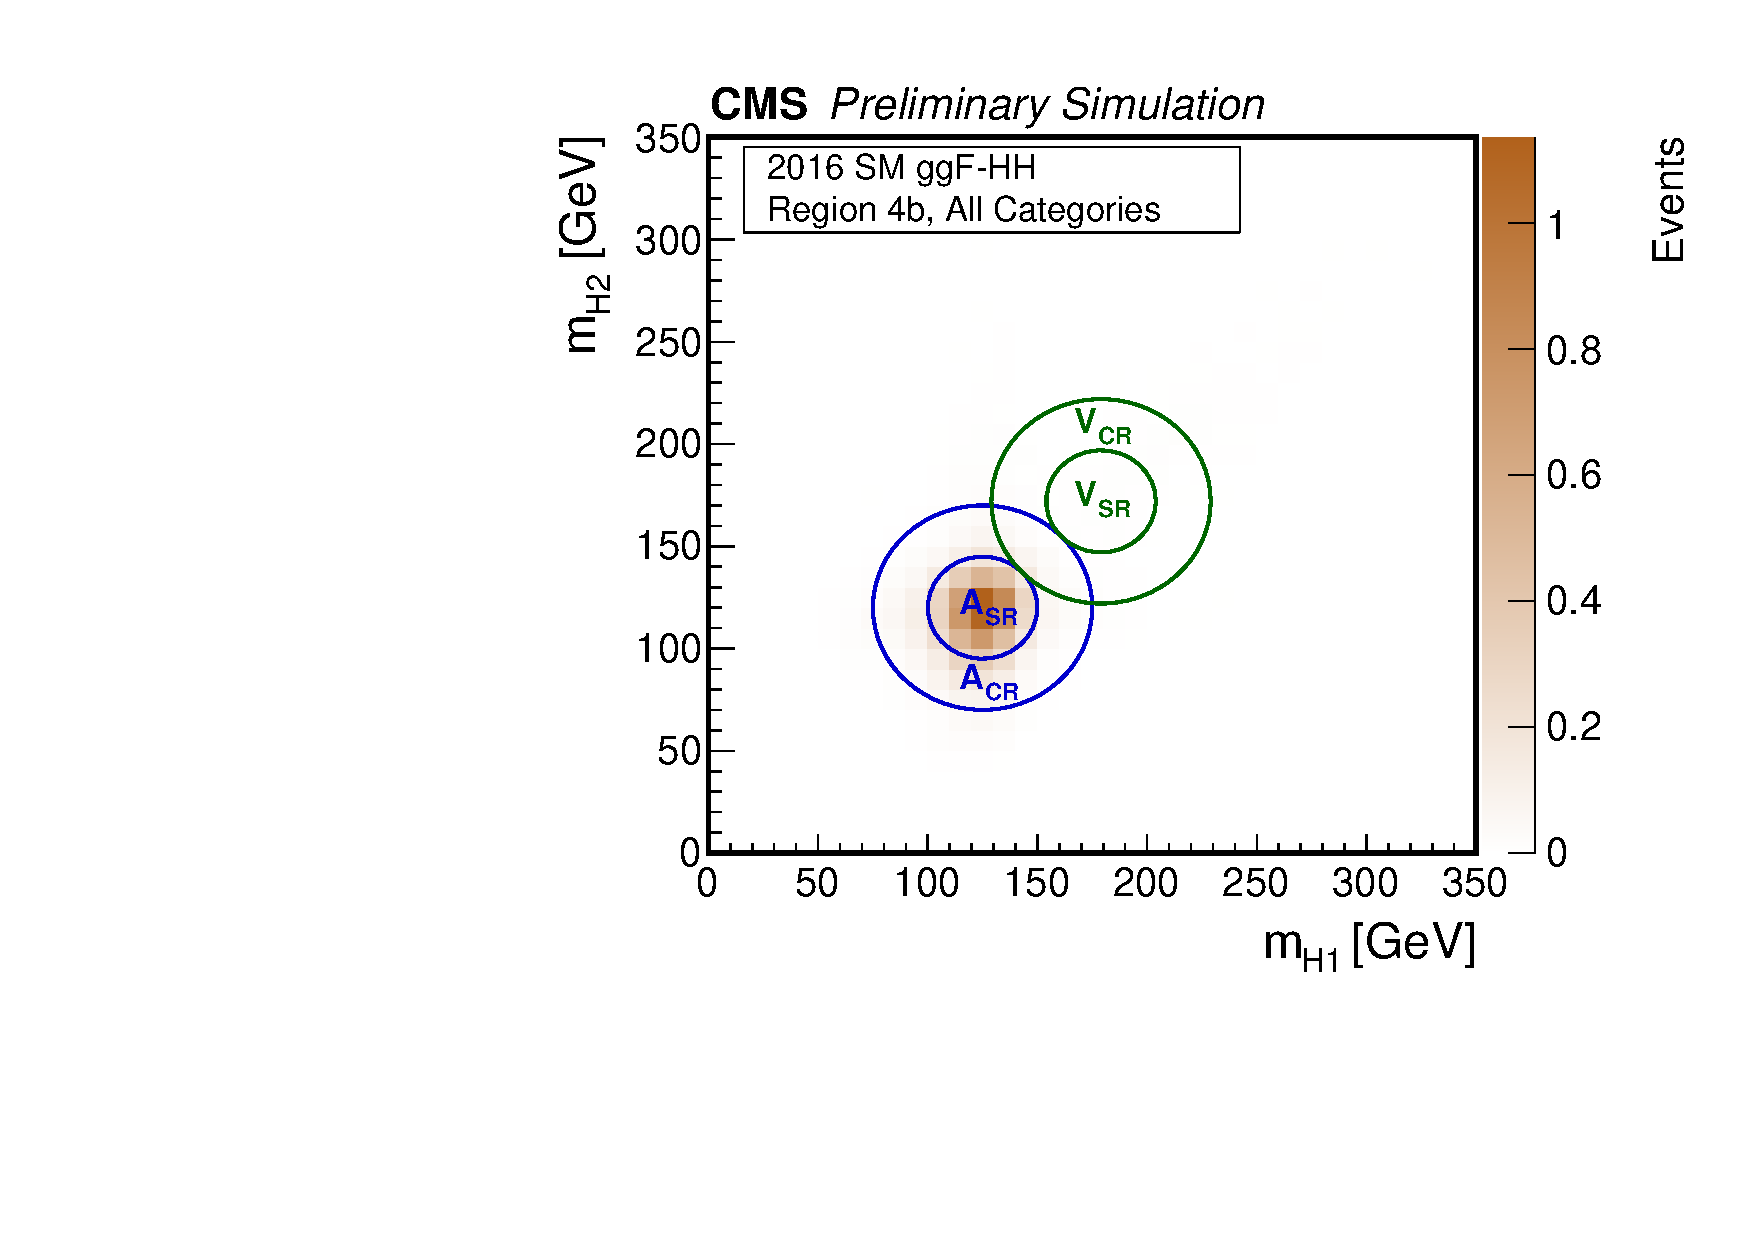
\includegraphics[width=0.45\linewidth]{Figures/AnalysisStrategy/eventselection/regions/CMS-PAS-HIG-20-005_Figure-aux_002-a.pdf}}
\subfloat[]{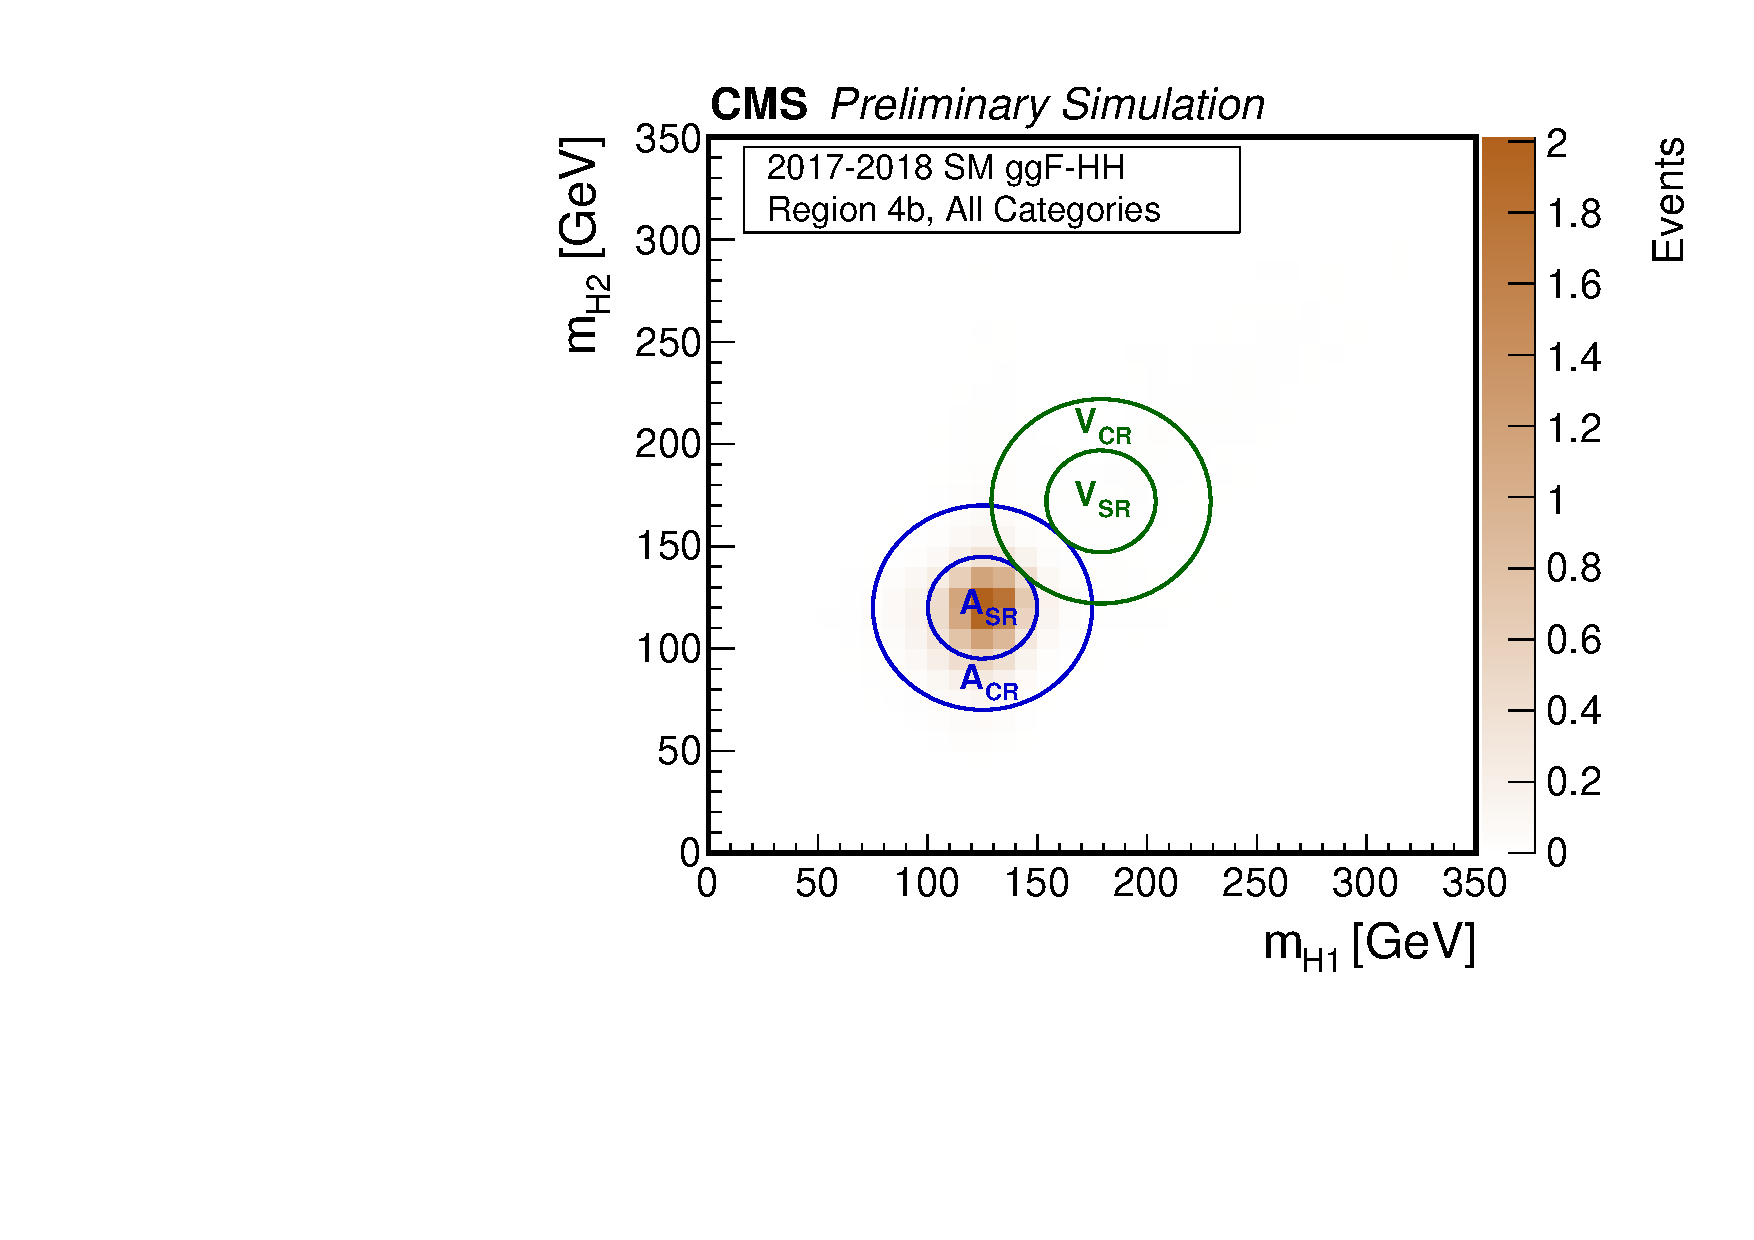
\includegraphics[width=0.45\linewidth]{Figures/AnalysisStrategy/eventselection/regions/CMS-PAS-HIG-20-005_Figure-aux_002-b.pdf}}\\
\subfloat[]{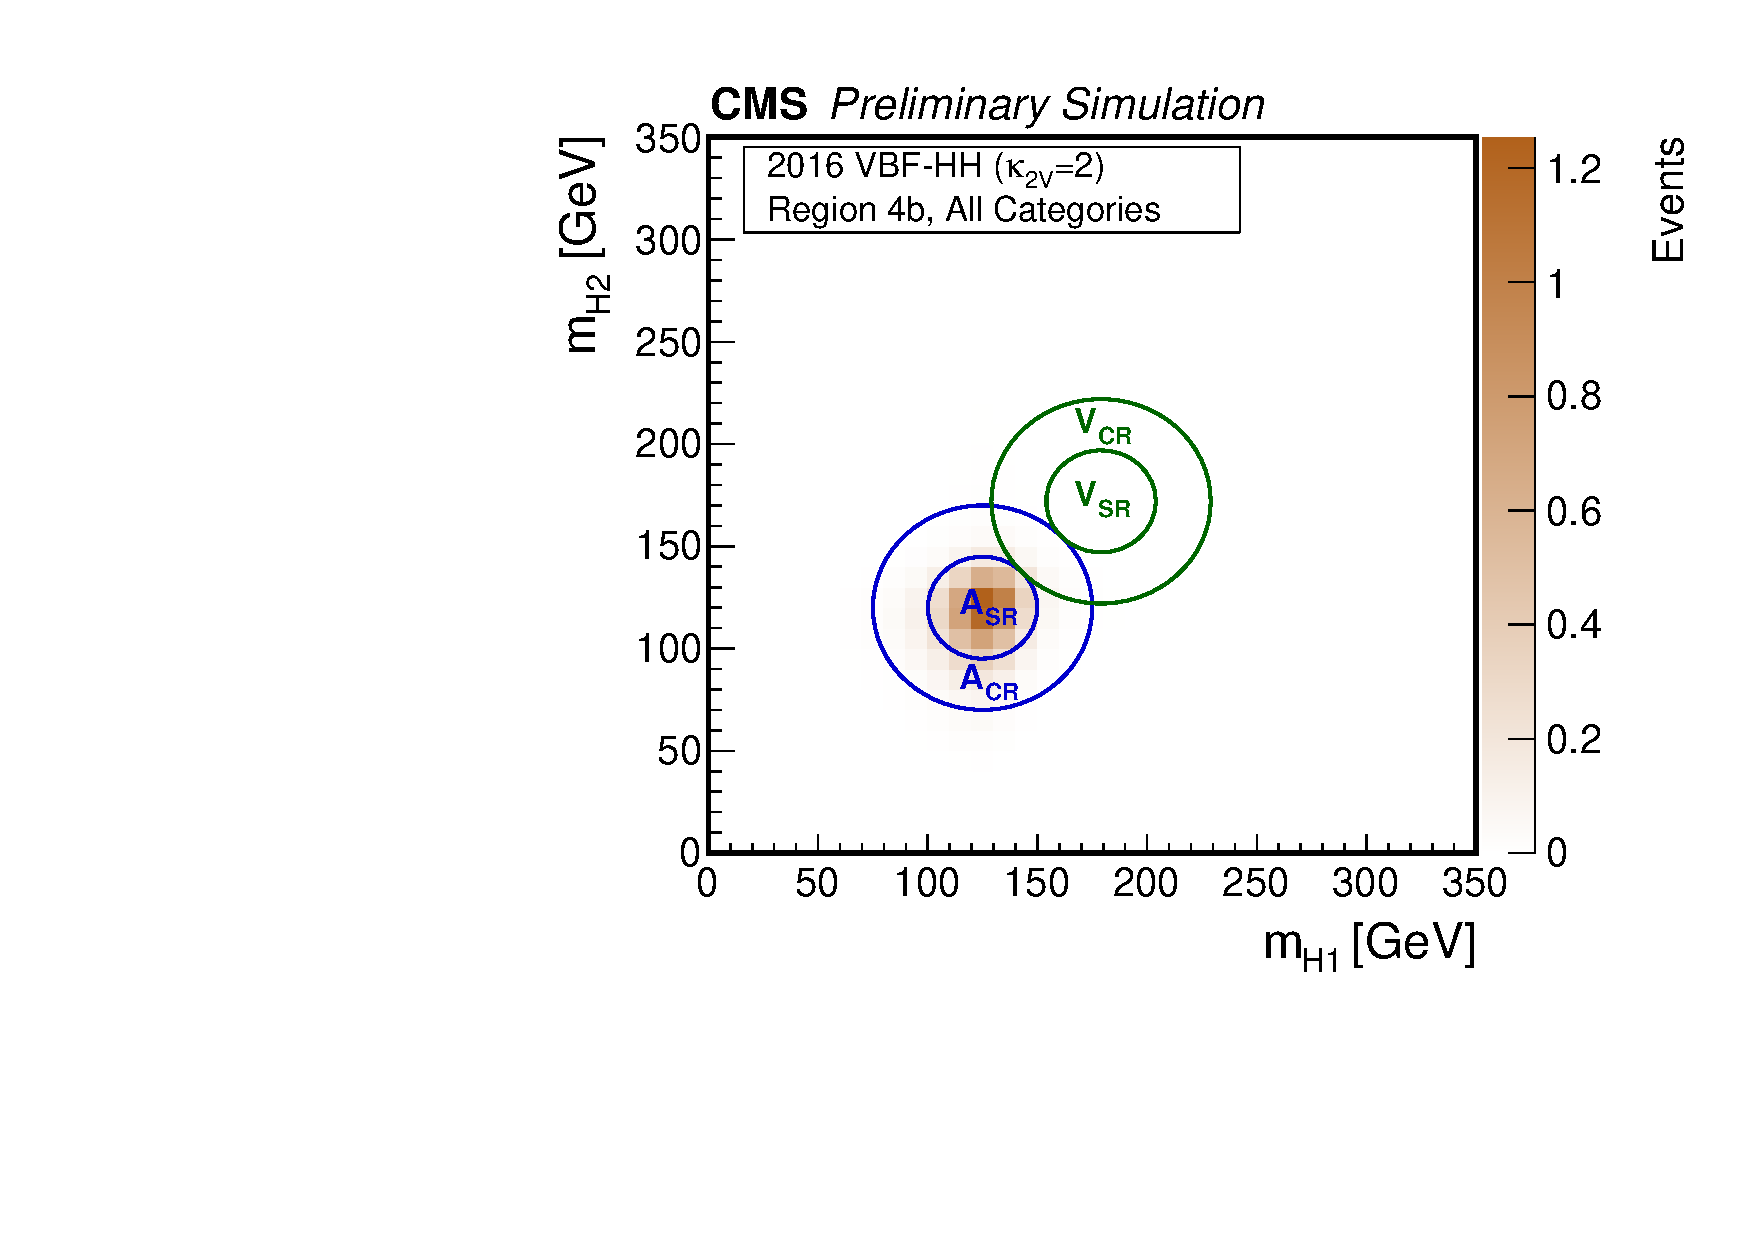
\includegraphics[width=0.45\linewidth]{Figures/AnalysisStrategy/eventselection/regions/CMS-PAS-HIG-20-005_Figure-aux_002-c.pdf}}
\subfloat[]{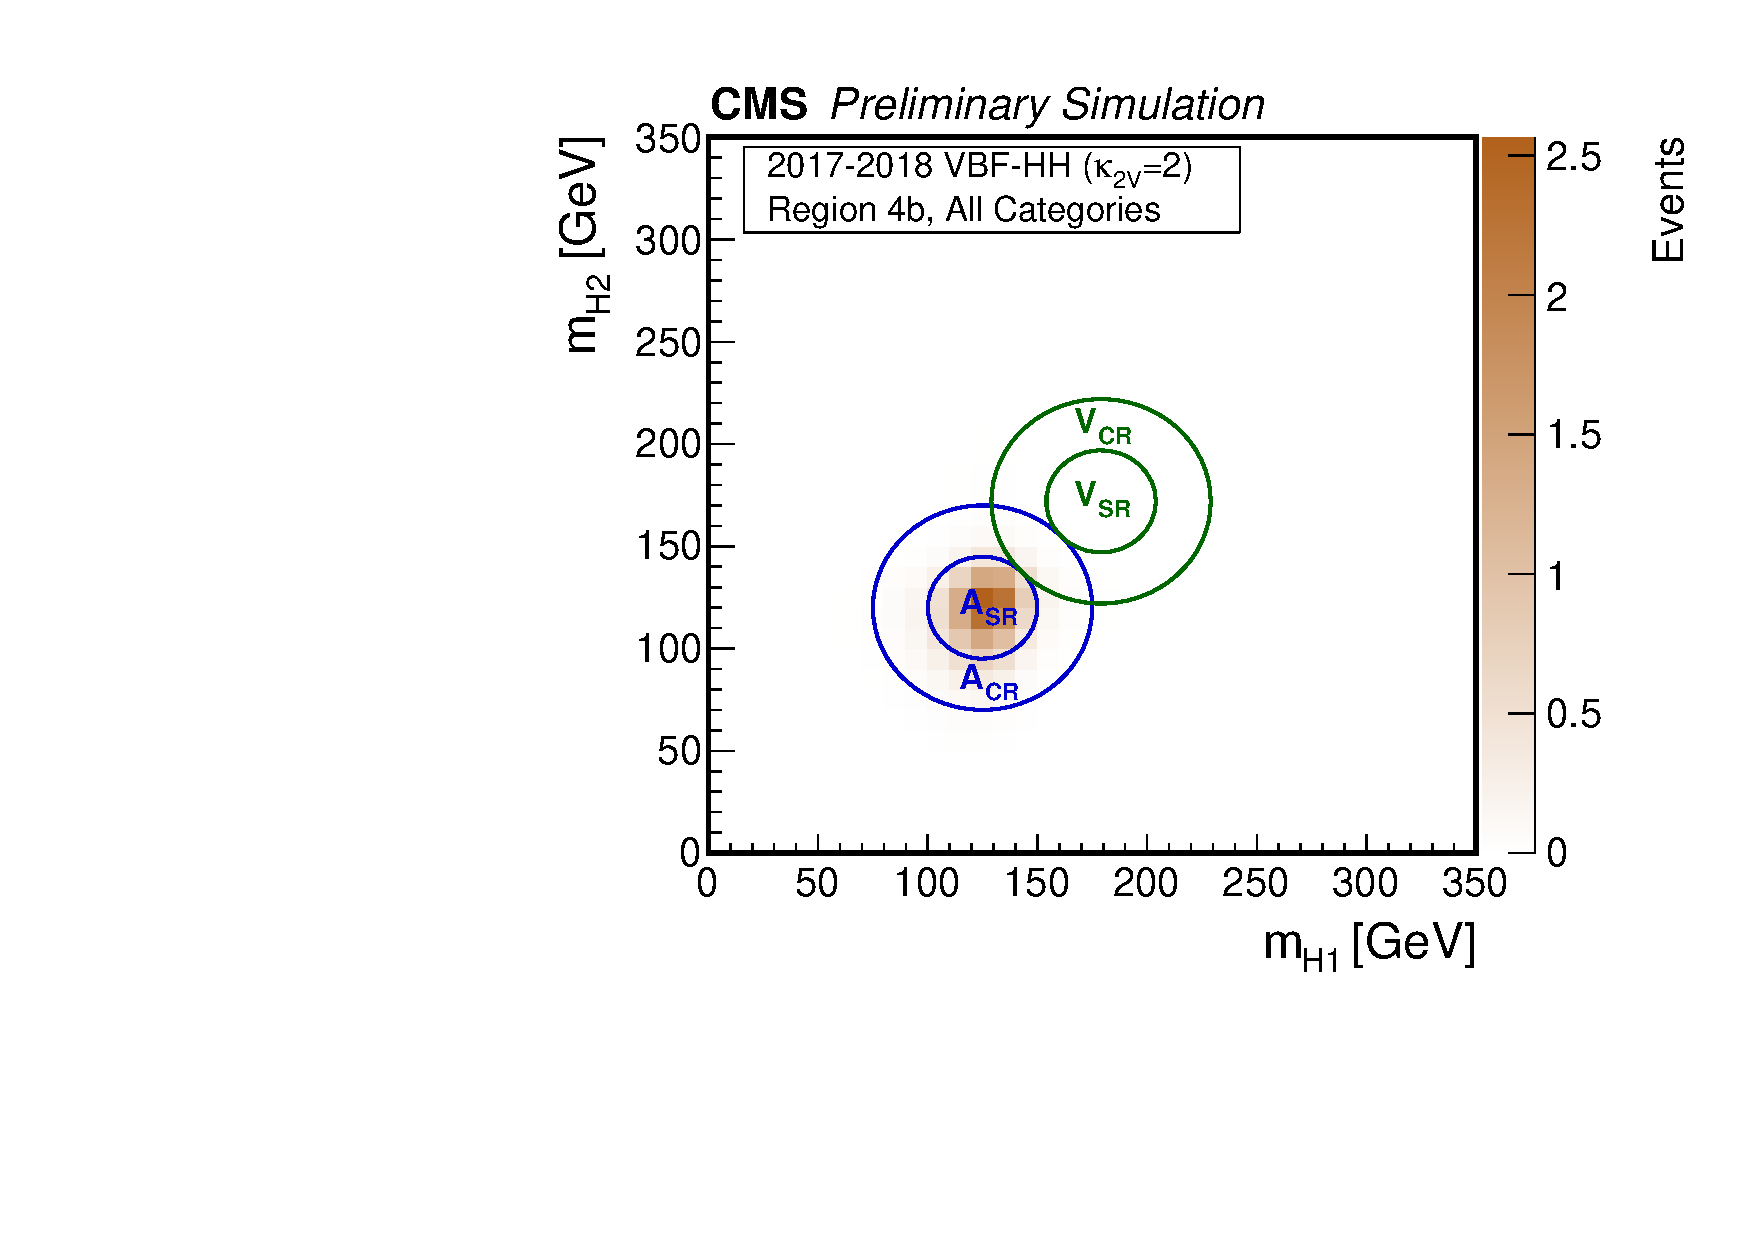
\includegraphics[width=0.45\linewidth]{Figures/AnalysisStrategy/eventselection/regions/CMS-PAS-HIG-20-005_Figure-aux_002-d.pdf}}
\caption[Distribution of the preselected signal events in the $\hfstm$-$\hsndm$ plane]{\label{event_selection:fig:vsrcrsignal}Distribution of the preselected signal events in the $\hfstm$-$\hsndm$ plane for A) SM ggF in 2016 conditions,  B) SM ggF in 2017-2018 conditions,  C) VBF with $\kvv=2$ in 2016 conditions, D) VBF with $\kvv=2$ in 2017-2018 conditions. The simulated events are normalized to their theoretical cross section and integrated luminosity. The definition of signal and control region in the analysis and validation region are presented.}
\end{figure}

A summary of the efficiencies to select ggF and VBF signals as a function of their coupling values is given in Figure~\ref{fig:eff_sel_ggf_vbf_2018} for the 2018 data-taking conditions. The efficiency lines illustrate the application of event requirements going from the online trigger to the analysis signal region. The 2016 and 2017 efficiencies have a similar behavior, as seen in Appendix~\ref{appendix:efficiencies}

\begin{figure}[htbp!]
\captionsetup[subfigure]{justification=centering}
\centering
\subfloat[]{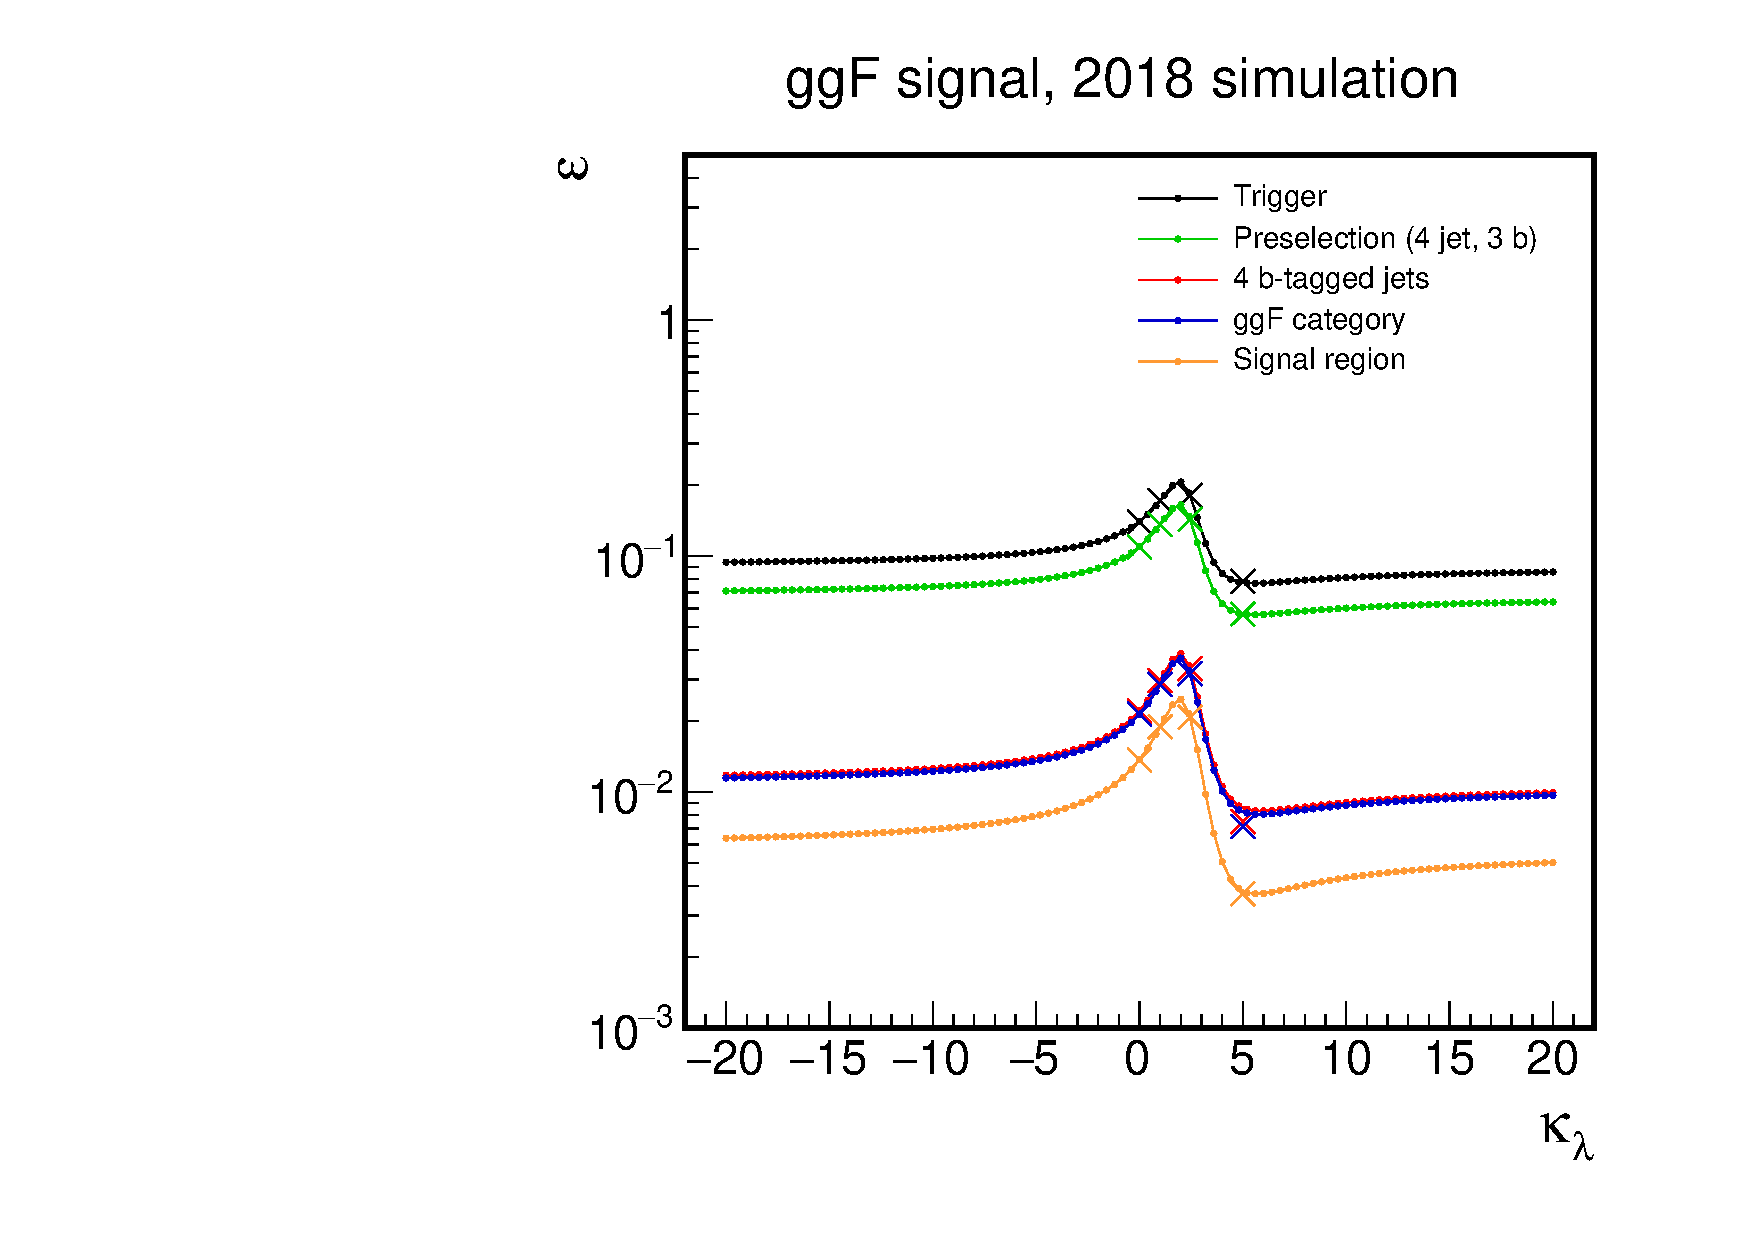
\includegraphics[width=0.45\linewidth]{Figures/AnalysisStrategy/eventselection/efficiencies/eff_2018_vs_klambda.pdf}}
\subfloat[]{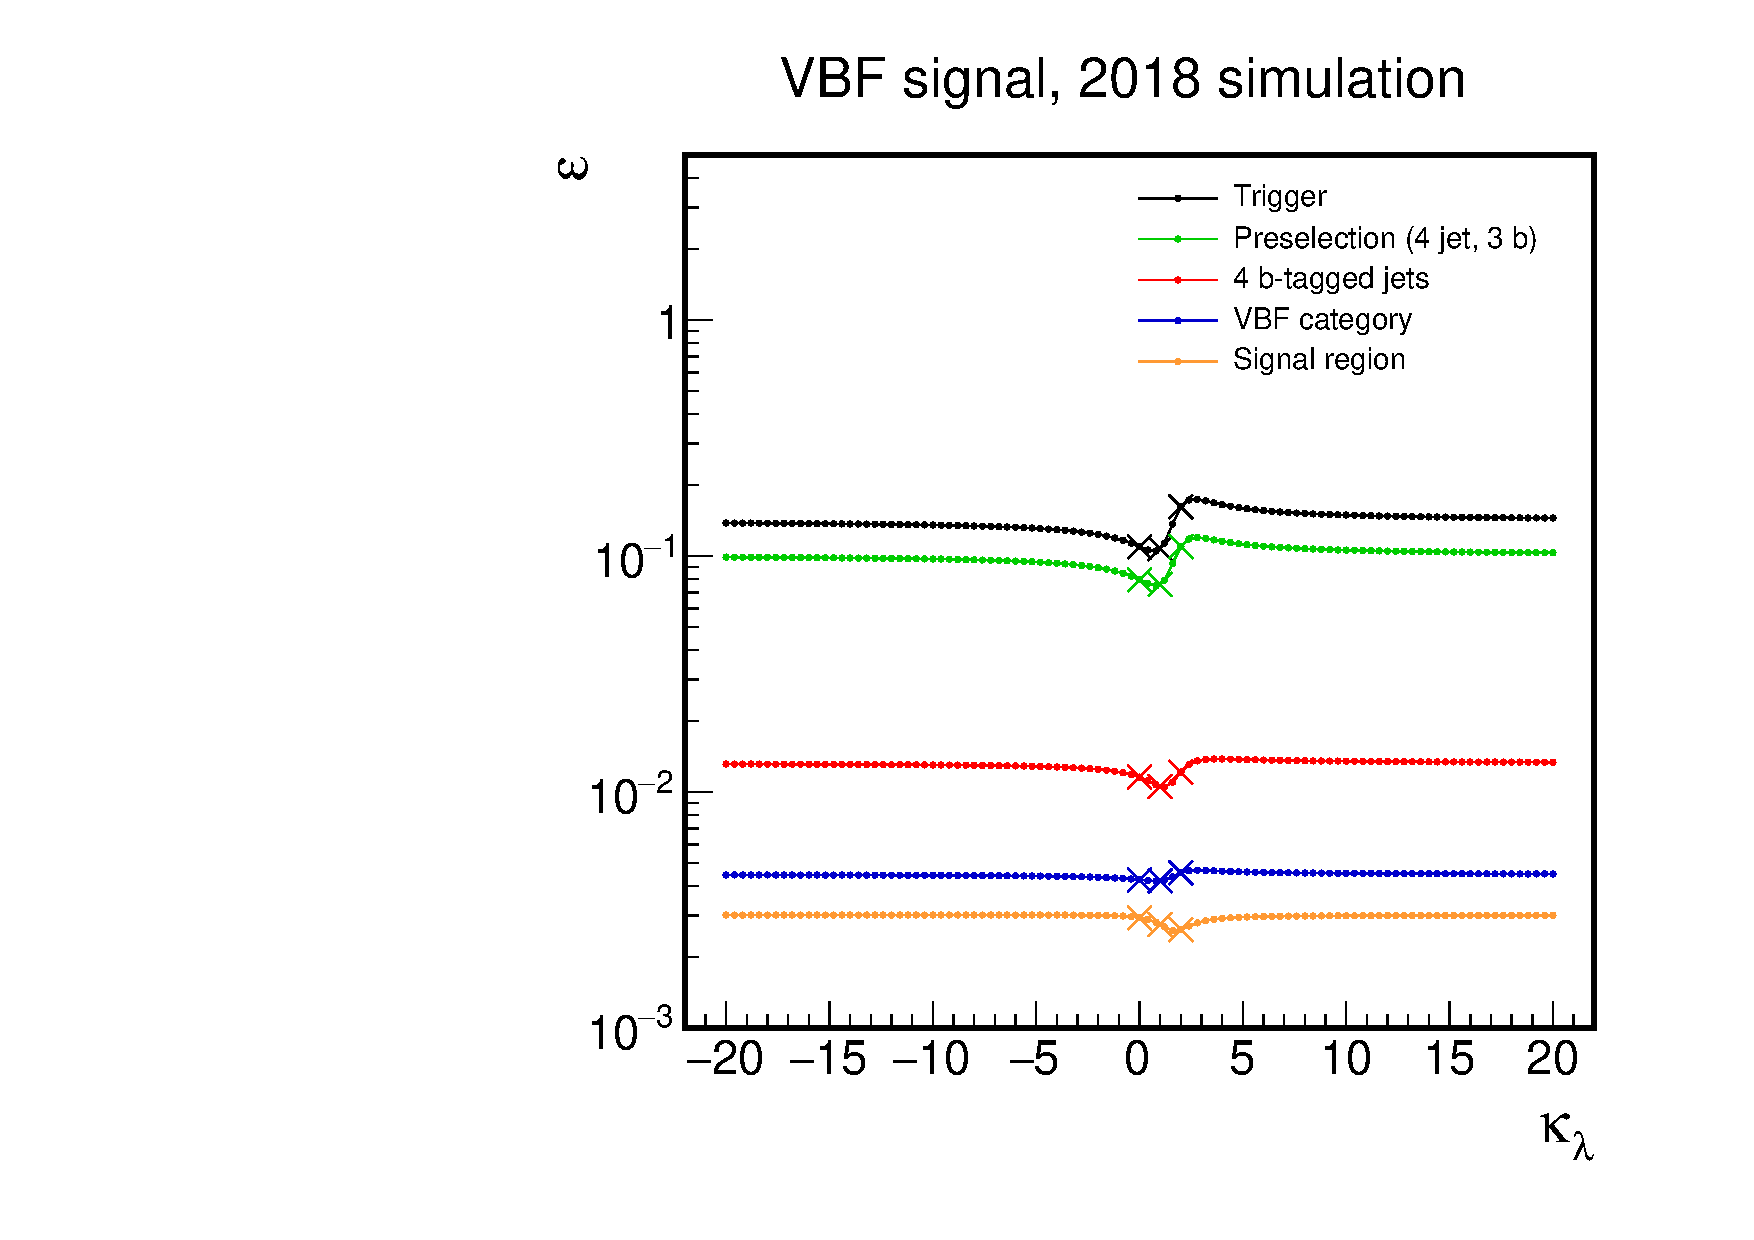
\includegraphics[width=0.45\linewidth]{Figures/AnalysisStrategy/eventselection/efficiencies/eff_2018_VBF_vs_kl.pdf}}\\
\subfloat[]{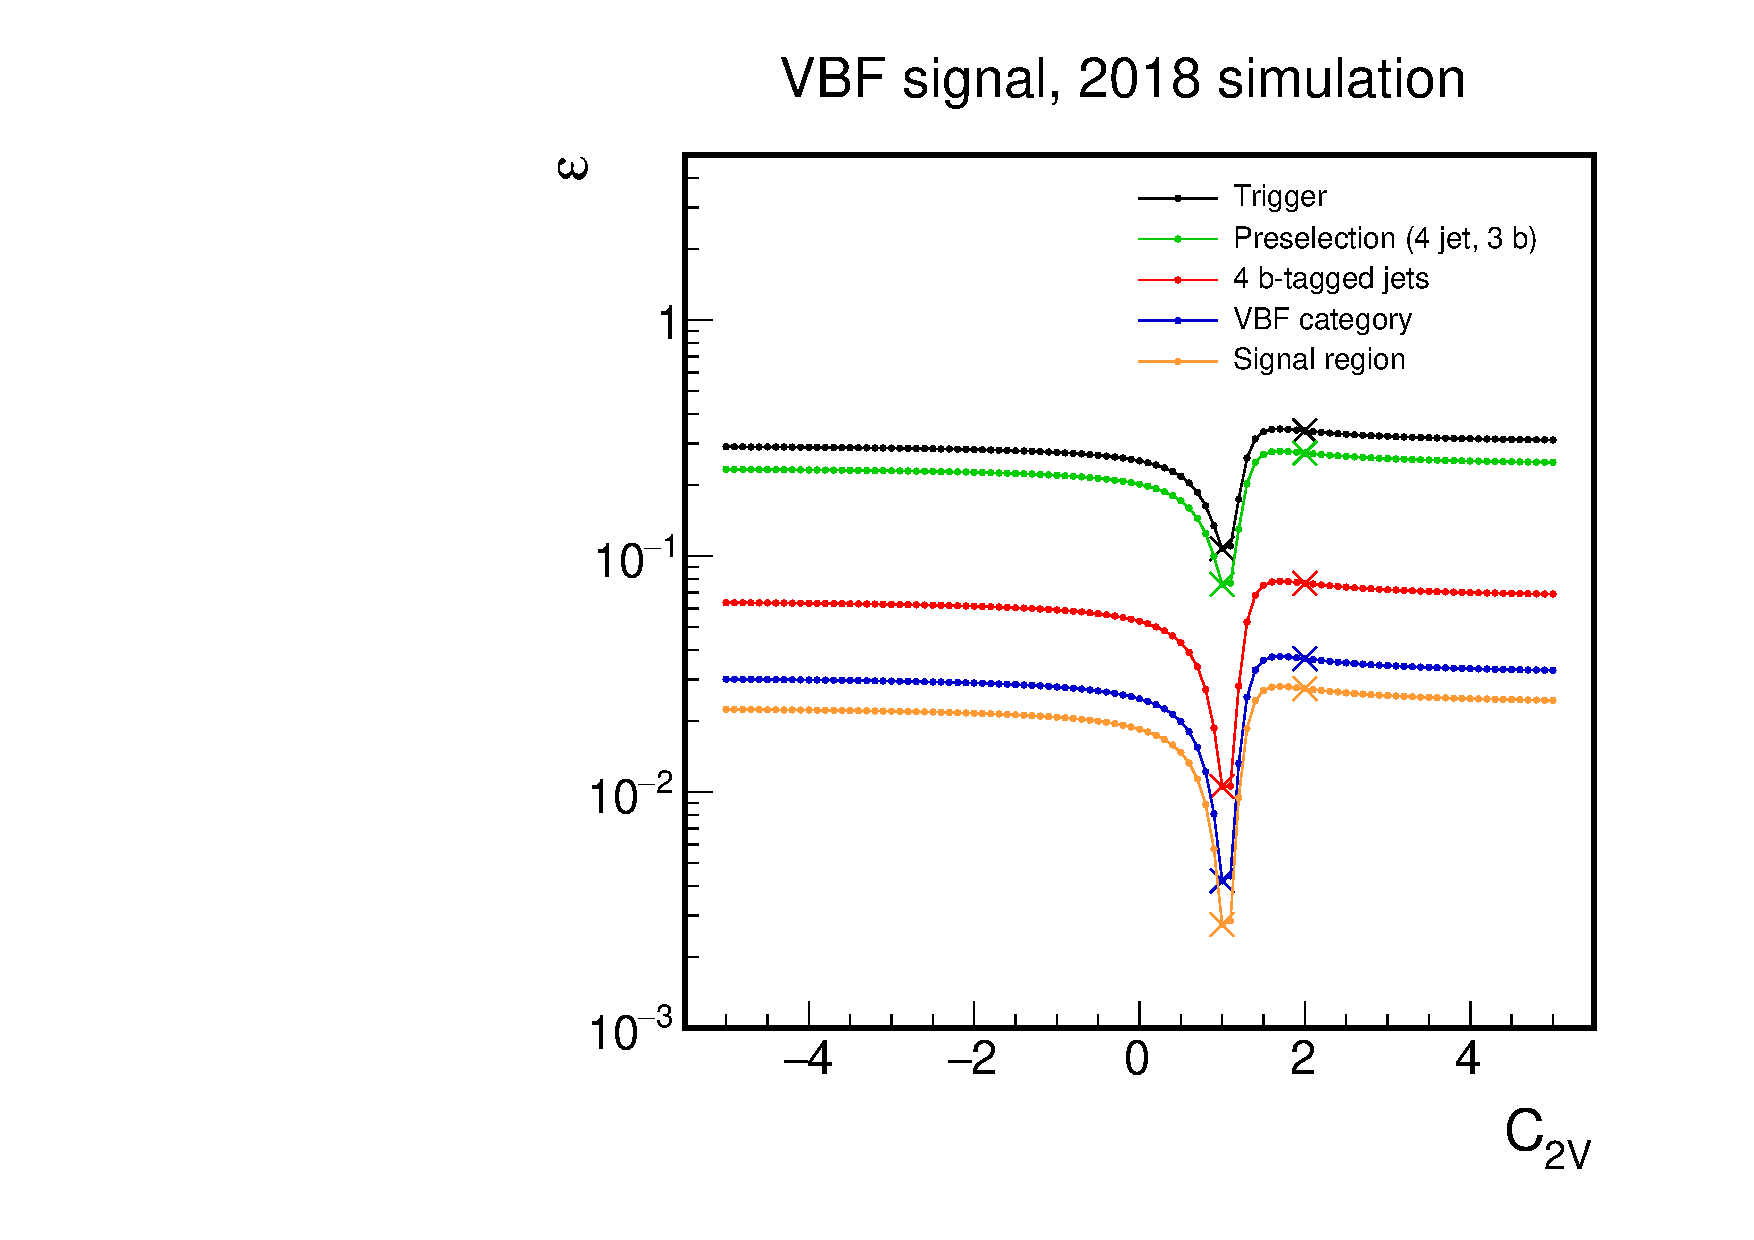
\includegraphics[width=0.45\linewidth]{Figures/AnalysisStrategy/eventselection/efficiencies/eff_2018_VBF_vs_C2V.pdf}}
\subfloat[]{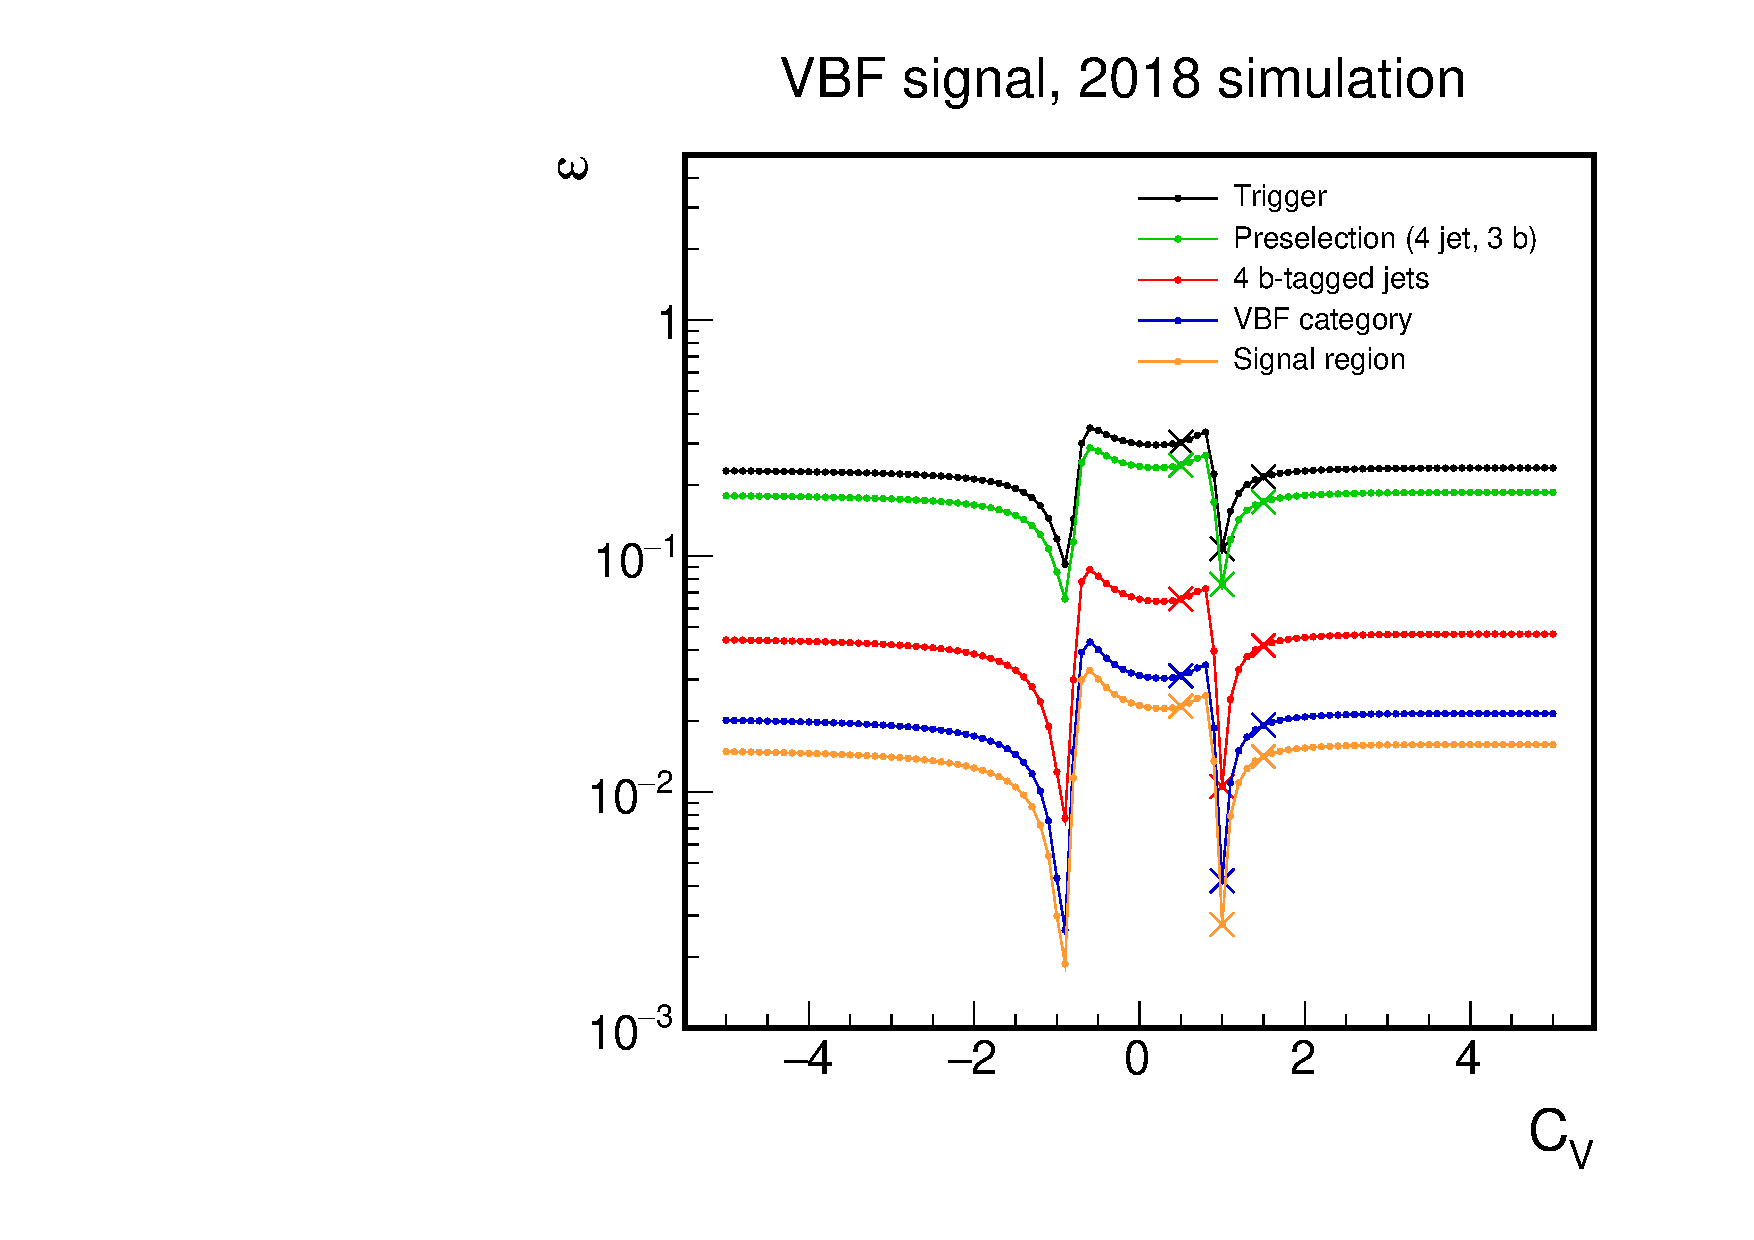
\includegraphics[width=0.45\linewidth]{Figures/AnalysisStrategy/eventselection/efficiencies/eff_2018_VBF_vs_CV.pdf}}
\caption[Selection efficiency ($\epsilon$) of the 2018 selections versus the ggF and VBF couplings]{Selection efficiency ($\epsilon$) of the 2018 selections versus the ggF and VBF couplings. $\epsilon$ vs $\kl$ for the A) ggF and B) VBF signals, C) $\epsilon$ versus $\kvv$ and D) $\epsilon$ versus $\kv$ for the VBF signals. In all figures, the couplings that are not displayed on the x-axis are assumed to be fixed to the SM value. The crosses indicate the values obtained directly from the simulated samples, serving as cross-check to the values computed with the signal modeling procedure (denoted by the full circles).}
\label{fig:eff_sel_ggf_vbf_2018}
\end{figure}


\clearpage

\section{Event Subcategorization}\label{sec:subcategories}

\subsection{Subcategory Boundaries} \label{subsec:optimization}
As seen in Chapter~\ref{hhproduction}, the coupling values can change the spectrum of the properties of the HH system. For this purpose, after events are classified into either the ggF or VBF categories, the next step is to split the categories into subcategories. This is to optimize further the analysis by targeting specific ggF and VBF signatures. The ggF and VBF analysis subcategories are defined based on $\hhm$ and ggFKiller score, respectively. The four subcategories are defined in Table~\ref{tab:subcategories}. The associated efficiencies as function of the couplings are illustrated in Figure~\ref{fig:eff_2016_subcategorization}.
\begin{table}[ht!]
\caption[Selection requirements used to define the event subcategorization]{\label{tab:subcategories}Selection requirements used to define the event subcategorization.}
\centering
\begin{tabularx}{\textwidth}{XX}
	\hline
	Subcategories                            & Selection requirements\\ [0.2em]
	\hline
	ggF Category 1 or 'Low-mass' ggF         & ggF category events, $\hhm<450$ GeV    \\ [0.2em]
	ggF Category 2 or 'High-mass' ggF        & ggF category events, $\hhm\geq450$ GeV \\ [0.2em]
	VBF Category 1 or 'SM-like' VBF          & VBF category events, 0.5$\leq$ggFKiller$<$0.970  \\ [0.2em]
	VBF Category 2 or 'Anomalous-$\kvv$' VBF & VBF category events, 0.970$\leq$ggFKiller$\leq$1 \\ [0.2em]
	\hline
\end{tabularx}
\end{table}

Two ggF subcategories are defined depending on the $\hhm$ kinematics. The boundary for the ggF categories is set at $\hhm=450$ GeV. This choice is driven by the ggF signal properties and the capability to validate the background model detailed in Section~\ref{sec:backgroundmodel}. For $\hhm>450$ GeV, ggF signals have similar distributions under the various $\kl$ hypotheses, as illustrated in Figure~\ref{event_selection:fig:obssubcategory} A), and where we expect their ratio to the SM curve to be flat. Consequently, we can train an optimal BDT output observable for $\kl$~hypotheses, and there is no gain in increasing further the threshold. Inversely, lowering the threshold much below 450 GeV poses a constraint on the $\hfstm$ and $\hsndm$ values in the low $\hhm$ category (or cat. 1) for background events, biasing them towards lower values. This effect impact how well `3b' and `4b' control region events populate the top-right corner of the ($\hfstm$, $\hsndm$) plane, reducing the statistical power to validate and trained a good validation background model. This effect is illustrated by different boundaries in Figure~\ref{event_selection:fig:ggfmasseffect}.

Two VBF subcategories are defined based on the SM-like and anomalous-$\kvv$ signatures. The VBF signal properties depending on the $\kvv$ are captured by the ggFKiller score, as seen in Figure~\ref{event_selection:fig:obssubcategory} B), and therefore, it is used to set the boundaries. There are two boundaries defined using the VBF couplings sensitivity as figure of merit: ($\beta_{1}$) The transition between ggF and VBF categories, and ($\beta_{2}$) the transition from SM-like and BSM-like kinematics. Here sensitivity means the upper limits on the signal strength parameter ($\mu$) using the background model and observables described in Section~\ref{sec:backgroundmodel} and Subsection~\ref{subsec:ggfvbfobservales}, respectively. The procedure is the following:
\begin{itemize}
    \item The value of $\beta_{2}$ is defined by studying the $\kvv = 2$ sensitivity in the VBF cat. 2 (a counting experiment) for thresholds starting from 0.900 in steps of 0.005. The boundary $\beta_{2}=0.97$ is found optimal for this analysis. 
    \item The value of the $\beta_{1}$ is found by testing ggFKiller points: 0.3, 0.4, 0.5, 0.6, 0.7. Most of the expected anomalous $\kvv = 2$ sensitivity is at high ggFKiller scores, thus the choice of the $\beta_{1}$ boundary only impacts the SM sensitivity. Consequently, the figure of merit is the SM VBF sensitivity in the SM-like subcategory. The tests showed the sensitivity improves by a few percent when increasing the thresholds. However, there is a significant amount of control region data loss affects our capability to build the data-driven background model. For example, the 2016 SM sensitivity improvements to up to 2\% (5\%) by requiring a value of 0.6 (0.7) instead of 0.5, but the loss of CR events is around 23\% (55\%). Therefore, ggFKiller=0.5 is the optimal boundary.
\end{itemize}

\begin{figure}[ht!]
\captionsetup[subfigure]{justification=centering}
\centering
\begin{center}
\subfloat[]{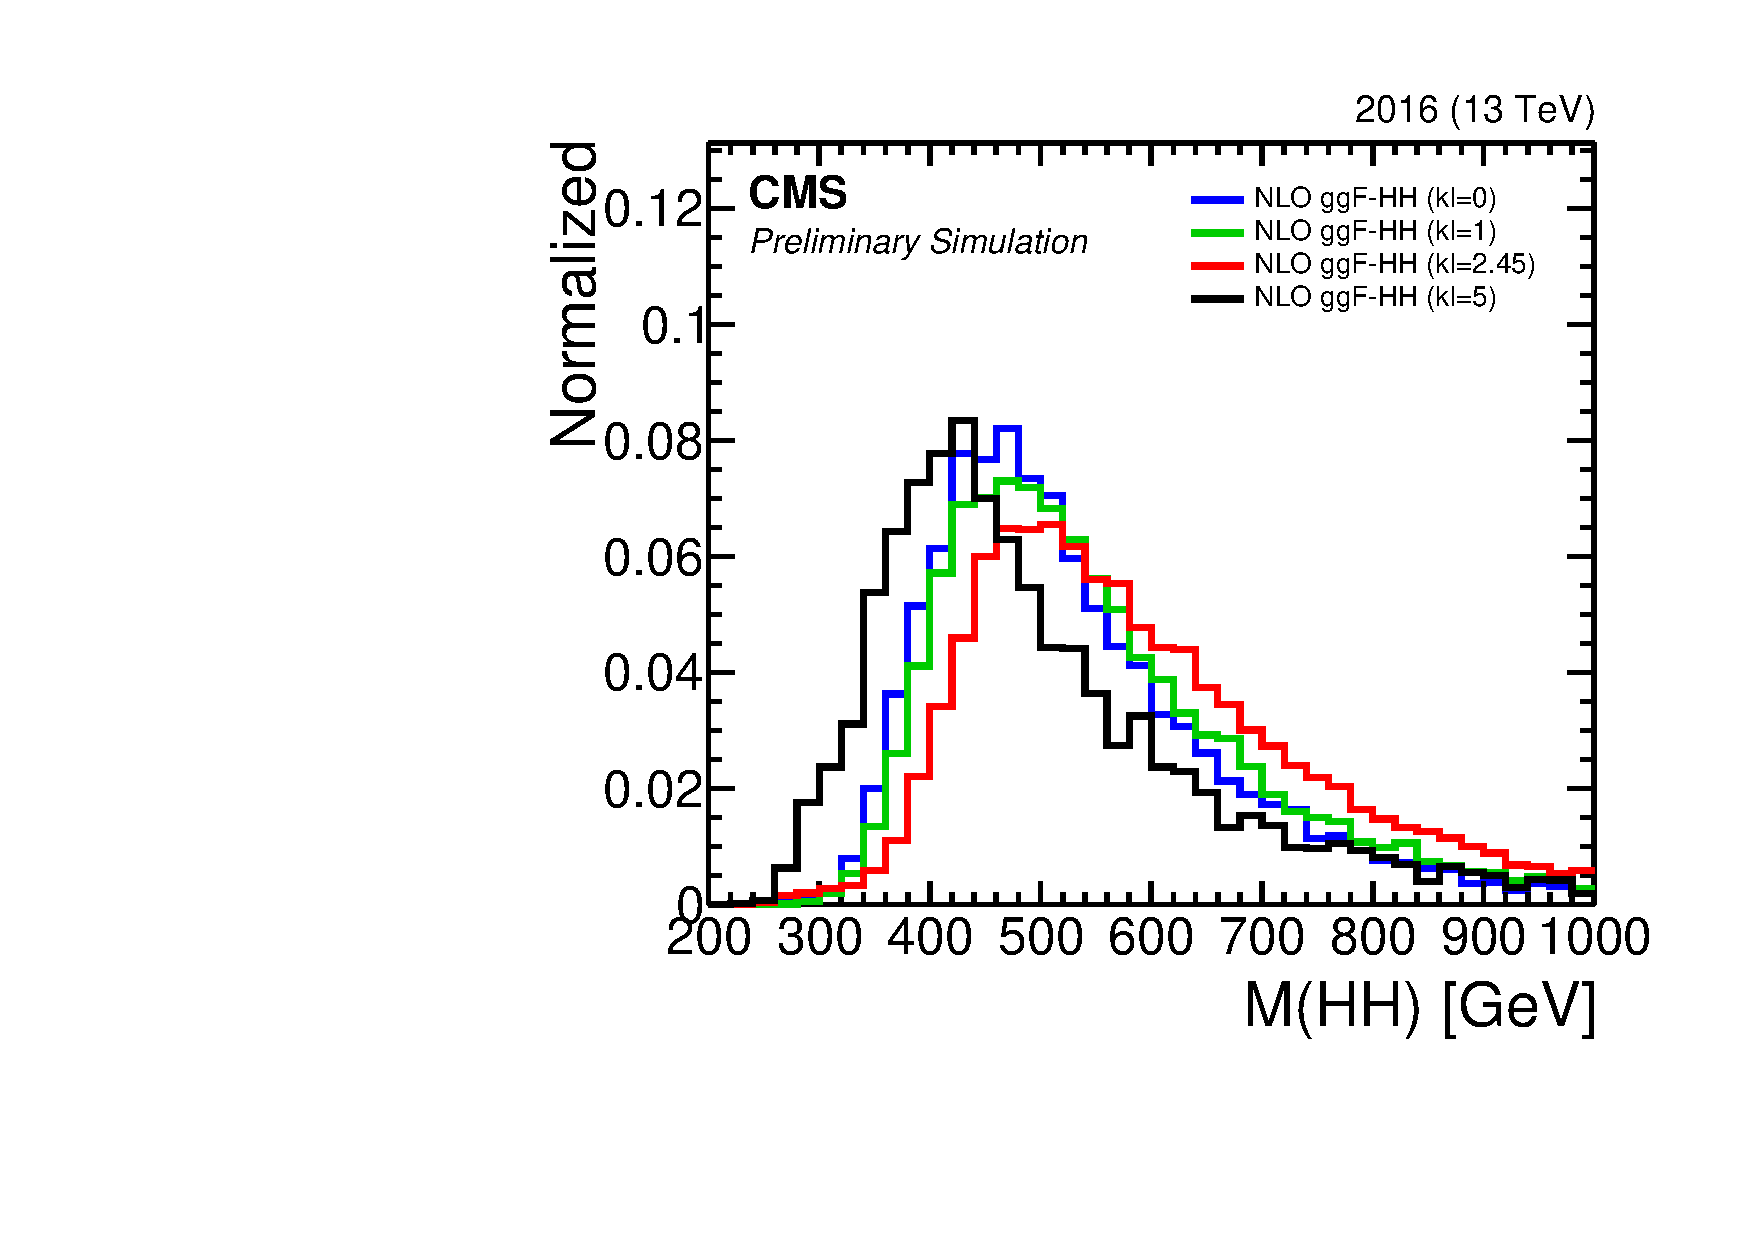
\includegraphics[width=0.45\linewidth]{Figures/AnalysisStrategy/eventselection/categorization/ggfcategories/plot_2016_h_HH_m.pdf}}
\subfloat[]{\includegraphics[width=0.45\linewidth]{Figures/AnalysisStrategy/eventselection/categorization/vbfcategories/plot_2016_h_GGFKiller_bins.pdf}}
\end{center}
\caption[Variables used to create ggF and VBF subcategories in the ggF and VBF signal region]{Variables used to create ggF and VBF subcategories in the ggF and VBF signal region. A) Invariant mass of the Higgs boson pair for ggF $\kl=0,1,2.45,5$ signals, B) ggFKiller score for VBF $\kvv=1,2$ signals. The simulated data-taking conditions correspond to 2016.}
\label{event_selection:fig:obssubcategory}
\end{figure}

\begin{figure}[ht!]
\captionsetup[subfigure]{justification=centering}
\centering
\begin{center}
\subfloat[]{\includegraphics[width=0.5\linewidth]{Figures/AnalysisStrategy/eventsubcategories/2dplot_ggf1_val_3b_375.pdf}}
\subfloat[]{\includegraphics[width=0.5\linewidth]{Figures/AnalysisStrategy/eventsubcategories/2dplot_ggf1_val_3b_400.pdf}}\\
\subfloat[]{\includegraphics[width=0.5\linewidth]{Figures/AnalysisStrategy/eventsubcategories/2dplot_ggf1_val_3b_425.pdf}}
\subfloat[]{\includegraphics[width=0.5\linewidth]{Figures/AnalysisStrategy/eventsubcategories/2dplot_ggf1_val_3b_450.pdf}}
\end{center}
\caption[Distribution of data events in the ggF category 1 in the ($\hfstm$, $\hsndm$) plane for the $\mathrm{V_{CR}(3b)}$ region using different $\hhm$ thresholds]{Distribution of data events in the ggF category 1 in the ($\hfstm$, $\hsndm$) plane for the $\mathrm{V_{CR}(3b)}$ region using different mass thresholds (in GeV). A) 375, B) 400, C) 425, and D) 450.}
\label{event_selection:fig:ggfmasseffect}
\end{figure}

\begin{figure}[ht!]
\captionsetup[subfigure]{justification=centering}
\begin{center}
\subfloat[]{\includegraphics[width=0.5\linewidth]{Figures/AnalysisStrategy/eventselection/efficiencies/frac_categ_2016_GGF_vs_kl.pdf}} 
\subfloat[]{\includegraphics[width=0.5\linewidth]{Figures/AnalysisStrategy/eventselection/efficiencies/frac_categ_2016_VBF_vs_C2V.pdf}} \\
\subfloat[]{\includegraphics[width=0.5\linewidth]{Figures/AnalysisStrategy/eventselection/efficiencies/frac_categ_2016_VBF_vs_CV.pdf}} 
\subfloat[]{\includegraphics[width=0.5\linewidth]{Figures/AnalysisStrategy/eventselection/efficiencies/frac_categ_2016_VBF_vs_kl.pdf}} \\
\end{center}
\caption[Performance of the production mode subcategorization as function of the ggF and VBF couplings]{Performance of the production mode subcategorization versus the ggF and VBF couplings. A) Fraction of ggF signal events from the ggF Category in the low-mass ggF subcategory and high-mass subcategory as a function of $\kl$. D/C/D) Fraction of VBF signal events from the VBF category classified in the SM-like subcategory and anomalous-$\kvv$ (BSM) subcategory as function of the $\kvv/\kv/\kl$ coupling. The crosses indicate the values obtained directly from the simulated samples, serving as cross-check to the values computed with the signal modeling procedure (denoted by the full circles). The simulated data-taking conditions correspond to 2016.}
\label{fig:eff_2016_subcategorization}
\end{figure}

\clearpage
\subsection{Signal Extraction Observables}~\label{subsec:ggfvbfobservales}
Optimal observables are chosen for each subcategory of the data analysis to obtain the final results presented in Chapter~\ref{chapter:results}. For ggF categories, the observable is the distribution of a multidimensional variable that aims at separating the signal and background events by combining the information of angular correlations, object kinematic properties, and object quality variables. The chosen multivariate analysis (MVA) algorithm is a Boosted Decision Tree (BDT) implemented in the XGBoost package~\cite{xgboost}. The training of these BDTs is possible due to rich variable information and the large number of data-driven background events (presented in Chapter~\ref{chapter:modeling}). 

The BDT outputs are trained per category and per datasets. The signal and background samples are the SM ggF model and the data-driven background model, respectively. The BDT is built using the  16 input variables listed in Table~\ref{strategy:bdtinputs}. Furthermore, Figures~\ref{discriminant:fig:bdt1variables20172018} and \ref{discriminant:fig:bdt2variables20172018} show the distributions of the signal and background for 2017-2018 ggF category 1 and ggF category 2, respectively. The equivalent distributions for 2016 are presented in Appendix~\ref{appendix:signalobs}.

\begin{table}[htbp!]
\caption[BDT input variables in ggF Category 1 and ggF Category 2]{\label{strategy:bdtinputs}BDT input variables in ggF Category 1 and ggF Category 2. $\mathrm{H_{1}}$ is the highest-$\pt$ Higgs candidate and $\mathrm{H_{2}}$ is the lowest-$\pt$ Higgs candidate.}
\centering
\begin{tabularx}{\textwidth}{X}
    \hline
    BDT input variables                          \\    
    \hline
    Mass of the $\mathrm{H_{1}}$ candidate, $\mathrm{M(H_{1})}$ \\
    Mass of the $\mathrm{H_{2}}$ candidate, $\mathrm{M(H_{2})}$  \\
    Mass of the Higgs pair system, $\hhm$  \\
    Transverse momentum of the $\mathrm{H_{1}}$ candidate, $\mathrm{P_{T}(H_{1})}$ \\
    Transverse momentum of the $\mathrm{H_{2}}$ candidate, $\mathrm{P_{T}(H_{2})}$ \\
    Pseudorapidity separation between the two Higgs candidates, $\Delta\eta\mathrm{(H_1,H_2)}$              \\   
    $\Delta R$ distance between two b jets of the $\mathrm{H_{1}}$ candidate, $\Delta\mathrm{R(H_{1}(bb))}$ \\
    $\Delta R$ distance between two b jets of the $\mathrm{H_{2}}$ candidate, $\Delta\mathrm{R(H_{2}(bb))}$ \\
    $|\mathrm{\cos}(\theta)\mathrm{^{*}~(H)}|$ in HH frame                               \\      
    $|\mathrm{\cos}(\theta)\mathrm{^{*}~(b)}|$ in $\mathrm{H_{1}}$ frame                 \\
    Sum of four b jets' regressed $\pt$                                                  \\
    Transverse momentum of the HH system, $\mathrm{\pt(HH)}$                             \\
    Number of tight b-tags in 3 highest b-tags                                          \\
    Sum of 3b's resolution scores                                                        \\
    Minimal $\Delta R$ distance between two b jets, Min$|\Delta\mathrm{R(bb)}|$          \\
    Maximum pseudorapidity separation between two b jets, Max$|\Delta\eta\mathrm{(bb)}|$ \\
    \hline
\end{tabularx}
\end{table}

\clearpage

\begin{figure}[ht!]
\caption[Input variables for the BDT output training in the 2017-2018 ggF Category 1.]{Input variables for the BDT output training in the 2017-2018 ggF Category 1. The SM ggF (signal) is in solid red, whereas the data-driven background modeling is in solid blue.}
\label{discriminant:fig:bdt1variables20172018}
\begin{center}
\includegraphics[width=0.24\linewidth]{Figures/AnalysisStrategy/signalobservables/ggfcategories//20172018ggfmva1/plot_20172018_h_abs_costh_H1_ggfcm.pdf}
\includegraphics[width=0.24\linewidth]{Figures/AnalysisStrategy/signalobservables/ggfcategories//20172018ggfmva1/plot_20172018_h_H1_bb_deltaR.pdf}
\includegraphics[width=0.24\linewidth]{Figures/AnalysisStrategy/signalobservables/ggfcategories//20172018ggfmva1/plot_20172018_h_h1h2_deltaEta.pdf}
\includegraphics[width=0.24\linewidth]{Figures/AnalysisStrategy/signalobservables/ggfcategories//20172018ggfmva1/plot_20172018_h_H1_m.pdf}\\
\includegraphics[width=0.24\linewidth]{Figures/AnalysisStrategy/signalobservables/ggfcategories//20172018ggfmva1/plot_20172018_h_H1_pt.pdf}
\includegraphics[width=0.24\linewidth]{Figures/AnalysisStrategy/signalobservables/ggfcategories//20172018ggfmva1/plot_20172018_h_H2_bb_deltaR.pdf}
\includegraphics[width=0.24\linewidth]{Figures/AnalysisStrategy/signalobservables/ggfcategories//20172018ggfmva1/plot_20172018_h_H2_m.pdf}
\includegraphics[width=0.24\linewidth]{Figures/AnalysisStrategy/signalobservables/ggfcategories//20172018ggfmva1/plot_20172018_h_H2_pt.pdf}\\
\includegraphics[width=0.24\linewidth]{Figures/AnalysisStrategy/signalobservables/ggfcategories//20172018ggfmva1/plot_20172018_h_HH_m.pdf}
\includegraphics[width=0.24\linewidth]{Figures/AnalysisStrategy/signalobservables/ggfcategories//20172018ggfmva1/plot_20172018_h_HH_pt.pdf}
\includegraphics[width=0.24\linewidth]{Figures/AnalysisStrategy/signalobservables/ggfcategories//20172018ggfmva1/plot_20172018_h_sum_3b_bres.pdf}
\includegraphics[width=0.24\linewidth]{Figures/AnalysisStrategy/signalobservables/ggfcategories//20172018ggfmva1/plot_20172018_h_sum_4b_pt.pdf}\\
\includegraphics[width=0.24\linewidth]{Figures/AnalysisStrategy/signalobservables/ggfcategories//20172018ggfmva1/plot_20172018_h_abs_costh_H1_b1_h1cm.pdf}
\includegraphics[width=0.24\linewidth]{Figures/AnalysisStrategy/signalobservables/ggfcategories//20172018ggfmva1/plot_20172018_h_min_4b_deltaR.pdf}
\includegraphics[width=0.24\linewidth]{Figures/AnalysisStrategy/signalobservables/ggfcategories//20172018ggfmva1/plot_20172018_h_max_4b_deltaEta.pdf}
\includegraphics[width=0.24\linewidth]{Figures/AnalysisStrategy/signalobservables/ggfcategories//20172018ggfmva1/plot_20172018_h_nBtagTight.pdf}
\end{center}
\end{figure}

\clearpage

\begin{figure}[ht!]
\caption[Input variables for the BDT output training in the 2017-2018 ggF Category 2]{Input variables for the BDT output training in the 2017-2018 ggF Category 2. The SM ggF (signal) is in solid red, whereas the data-driven background modeling is in solid blue.}
\label{discriminant:fig:bdt2variables20172018}
\begin{center}
\includegraphics[width=0.24\linewidth]{Figures/AnalysisStrategy/signalobservables/ggfcategories//20172018ggfmva2/plot_20172018_h_abs_costh_H1_ggfcm.pdf}
\includegraphics[width=0.24\linewidth]{Figures/AnalysisStrategy/signalobservables/ggfcategories//20172018ggfmva2/plot_20172018_h_H1_bb_deltaR.pdf}
\includegraphics[width=0.24\linewidth]{Figures/AnalysisStrategy/signalobservables/ggfcategories//20172018ggfmva2/plot_20172018_h_h1h2_deltaEta.pdf}
\includegraphics[width=0.24\linewidth]{Figures/AnalysisStrategy/signalobservables/ggfcategories//20172018ggfmva2/plot_20172018_h_H1_m.pdf}\\
\includegraphics[width=0.24\linewidth]{Figures/AnalysisStrategy/signalobservables/ggfcategories//20172018ggfmva2/plot_20172018_h_H1_pt.pdf}
\includegraphics[width=0.24\linewidth]{Figures/AnalysisStrategy/signalobservables/ggfcategories//20172018ggfmva2/plot_20172018_h_H2_bb_deltaR.pdf}
\includegraphics[width=0.24\linewidth]{Figures/AnalysisStrategy/signalobservables/ggfcategories//20172018ggfmva2/plot_20172018_h_H2_m.pdf}
\includegraphics[width=0.24\linewidth]{Figures/AnalysisStrategy/signalobservables/ggfcategories//20172018ggfmva2/plot_20172018_h_H2_pt.pdf}\\
\includegraphics[width=0.24\linewidth]{Figures/AnalysisStrategy/signalobservables/ggfcategories//20172018ggfmva2/plot_20172018_h_HH_m.pdf}
\includegraphics[width=0.24\linewidth]{Figures/AnalysisStrategy/signalobservables/ggfcategories//20172018ggfmva2/plot_20172018_h_HH_pt.pdf}
\includegraphics[width=0.24\linewidth]{Figures/AnalysisStrategy/signalobservables/ggfcategories//20172018ggfmva2/plot_20172018_h_sum_3b_bres.pdf}
\includegraphics[width=0.24\linewidth]{Figures/AnalysisStrategy/signalobservables/ggfcategories//20172018ggfmva2/plot_20172018_h_sum_4b_pt.pdf}\\
\includegraphics[width=0.24\linewidth]{Figures/AnalysisStrategy/signalobservables/ggfcategories//20172018ggfmva2/plot_20172018_h_abs_costh_H1_b1_h1cm.pdf}
\includegraphics[width=0.24\linewidth]{Figures/AnalysisStrategy/signalobservables/ggfcategories//20172018ggfmva2/plot_20172018_h_min_4b_deltaR.pdf}
\includegraphics[width=0.24\linewidth]{Figures/AnalysisStrategy/signalobservables/ggfcategories//20172018ggfmva2/plot_20172018_h_max_4b_deltaEta.pdf}
\includegraphics[width=0.24\linewidth]{Figures/AnalysisStrategy/signalobservables/ggfcategories//20172018ggfmva2/plot_20172018_h_nBtagTight.pdf}
\end{center}
\end{figure}


\clearpage

A good practice is to avoid the introduction of a bias on the BDT distribution for background events by reusing the same training/test samples to evaluate the final results.  As it will be seen in Chapter~\ref{chapter:modeling}, the analysis sensitivity is dominated by the background model uncertainties. If the background event samples are reduced due to the BDT training, then the statistical uncertainty on the background model will increase, and there will be direct impact on the final result. For this reason, a special training method is designed to allow for the 100\% of the background model to be used for the signal extraction. The procedure is summarized as follows:
\begin{enumerate}
  \item Prepare the expected signal (S) and background model (B) samples in the signal region
  \item Split the background model into two halves, denoted as B1 and B2 samples.
  \item A first classifier (C1) is trained using the signal S and the background B1 sample using the hyperparameter optimization procedure used for the ggFKiller score with nine grids. %(subsection~\ref{subsection:ggfkiller}) 
  \item A second classifier (C2) is trained with the signal (S) and the background model B2 samples using the exact same resulting hyperparameters of the classifier C1. 
\end{enumerate}

Detailed information of the training results of the C1 and C2 classifiers is presented in Appendix~\ref{appendix:signalobs}. Next, compatibility checks are performed to ensure that the C1 and C2 will give the same performance in any event sample: (1) The ROC-AUC curves associated to the evaluation of the classifier C1 in the S and B1 samples and the evaluation of the classifier C2 in the S and B2 samples are compatible; (2) The ROC-AUC curves associated to the evaluation of the classifier C1 in the S and B2 samples and the evaluation of the classifier C2 in the S and B1 samples are compatible; (3) The distributions have similar shapes when evaluating the S (B1) samples using classifier C2 versus the S (B2) samples using classifier C1.

The compatibility checks show that the two classifiers are compatible and give the same results. This is illustrated for the 2017-2018 dataset in Figure~\ref{discriminant:fig:c1c2_checks_20172018}. Lastly, for each ggF category and dataset, the BDT output used for the final results is built by evaluating the C1 and C2 classifiers using the following recipe: 
\begin{itemize}
  \item Background model events in sample B1: 100\% uses classifier C2 
  \item Background model events in sample B2: 100\% uses classifier C1
  \item Simulated events: A 50\% uses classifier C1 and the other 50\% uses classifier C2
  \item Observed data events: A 50\% uses classifier C1 and the other 50\% uses classifier C2
\end{itemize}

\begin{figure}[ht!]
\caption[Compatibility checks on the classifiers used for the 2017-2018 ggF observables]{Compatibility checks on the classifiers used for the 2017-2018 ggF observables. A) Category 1 and B) Category 2. The left figure shows the ROC-AUC curves performance checks. The right figure illustrates the distributions for signal S and background model B1 (B2) samples using the C2 (C1) classifier.}
\label{discriminant:fig:c1c2_checks_20172018}
\captionsetup[subfigure]{justification=centering}
\begin{center}
\subfloat[]{
\includegraphics[width=0.33\linewidth]{Figures/AnalysisStrategy/signalobservables/ggfcomparisons/20172018/cat1_20172018MVA1B1_VS_20172018MVA1B2_roc.png}
\includegraphics[width=0.33\linewidth]{Figures/AnalysisStrategy/signalobservables/ggfcomparisons/20172018/ggfmva1_20172018MVA1B1VS20172018MVA1B2_score_output.png}}\\
\subfloat[]{\includegraphics[width=0.33\linewidth]{Figures/AnalysisStrategy/signalobservables/ggfcomparisons/20172018/cat2_20172018MVA2B1_VS_20172018MVA2B2_roc.png}
\includegraphics[width=0.33\linewidth]{Figures/AnalysisStrategy/signalobservables/ggfcomparisons/20172018/ggfmva2_20172018MVA2B1VS20172018MVA2B2_score_output.png}}\\
\end{center}
\end{figure}


For VBF categories, data-driven background model statistics is small when compared to the one of the ggF categories. This makes it challenging to prepare a BDT output, and consequently, a different strategy is followed. For VBF category 1, mass variables associated to the Higgs boson pairs are expected to have similar separation performance. The chosen variable is the invariant mass of the Higgs boson pair system ($\hhm$). For the VBF category 2, the expected number of background events is at the order of 5-20 events, depending on the dataset. Therefore, the observable is a single bin used to perform a counting experiment.